\documentclass[12pt,]{article}
%\usepackage{lmodern}  Melissa removed to deal with font rendering issue
\usepackage{amssymb,amsmath}
\usepackage{ifxetex,ifluatex}
\usepackage{fixltx2e} % provides \textsubscript

%Melissa removed the following section to deal with font rendering issue
%\ifnum 0\ifxetex 1\fi\ifluatex 1\fi=0 % if pdftex
%  \usepackage[T1]{fontenc}
%  \usepackage[utf8]{inputenc}
%%\else % if luatex or xelatex
%  \ifxetex
%    \usepackage{mathspec}
%  \else
%    \usepackage{fontspec}
%  \fi
%  \defaultfontfeatures{Ligatures=TeX,Scale=MatchLowercase}
%  \newcommand{\euro}{€}
%%%%%%\fi

% use upquote if available, for straight quotes in verbatim environments
\IfFileExists{upquote.sty}{\usepackage{upquote}}{}
% use microtype if available
\IfFileExists{microtype.sty}{%
\usepackage{microtype}
\UseMicrotypeSet[protrusion]{basicmath} % disable protrusion for tt fonts
}{}
\usepackage[margin=1in]{geometry}
\usepackage{hyperref}
\PassOptionsToPackage{usenames,dvipsnames}{color} % color is loaded by hyperref
\hypersetup{unicode=true,
            pdftitle={Status of California Scorpionfish (Scorpaena guttata) Off Southern California in 2017},
            pdfborder={0 0 0},
            breaklinks=true}
\urlstyle{same}  % don't use monospace font for urls
\usepackage{graphicx,grffile}
\makeatletter
\def\maxwidth{\ifdim\Gin@nat@width>\linewidth\linewidth\else\Gin@nat@width\fi}
\def\maxheight{\ifdim\Gin@nat@height>\textheight\textheight\else\Gin@nat@height\fi}
\makeatother
% Scale images if necessary, so that they will not overflow the page
% margins by default, and it is still possible to overwrite the defaults
% using explicit options in \includegraphics[width, height, ...]{}
\setkeys{Gin}{width=\maxwidth,height=\maxheight,keepaspectratio}
\setlength{\parindent}{0pt}
\setlength{\parskip}{6pt plus 2pt minus 1pt}
\setlength{\emergencystretch}{3em}  % prevent overfull lines
\providecommand{\tightlist}{%
  \setlength{\itemsep}{0pt}\setlength{\parskip}{0pt}}
\setcounter{secnumdepth}{5}

%%% Use protect on footnotes to avoid problems with footnotes in titles
\let\rmarkdownfootnote\footnote%
\def\footnote{\protect\rmarkdownfootnote}

%%% Change title format to be more compact
\usepackage{titling}

% Create subtitle command for use in maketitle
\newcommand{\subtitle}[1]{
  \posttitle{
    \begin{center}\large#1\end{center}
    }
}

\setlength{\droptitle}{-2em}
  \title{Status of California Scorpionfish (\emph{Scorpaena guttata}) Off
Southern California in 2017}
  \pretitle{\vspace{\droptitle}\centering\huge}
  \posttitle{\par}
  \author{}
  \preauthor{}\postauthor{}
  \date{}
  \predate{}\postdate{}


% This file contains all of the LaTeX packages you may need to compile the document
% Documentation for each package can be found onlines
\usepackage{tabularx}                                             % table environment providing flexibility
\usepackage{caption}                                              % for creating captions  
\usepackage{longtable}                                            % allows tables to span multiple pages
\usepackage{rotating}                                             % allows for sideways tables
\usepackage{float}                                                % floating environments; may not need in rmarkdown
\usepackage{placeins}                                             % keeps floats from moving
\usepackage{indentfirst}                                          % indents first paragraph of a section
\usepackage{mdwtab}                                               % continued float multi-page figure
\usepackage{enumerate}                                            % create lists
\usepackage{hyperref}                                             % highlight cross references
\hypersetup{colorlinks=true, urlcolor=blue, linktoc=page, linkcolor=blue, citecolor=blue} %define referencing colors
%\usepackage{makebox}                                             % make boxes around text
\usepackage[usenames,dvipsnames]{xcolor}                          % color name options
%\usepackage[space]{grffile}                                      % spaces in file name path
\usepackage{soul}                                                 % highlight text
\usepackage{enumitem}                                             % numbered lists
\usepackage{lineno}                                               % Line numbers; comment out for final
\usepackage{upquote}                                              % produce grave accent in latex
\usepackage{verbatim}                                             % produces verbatim results
\usepackage{fancyvrb}                                             % verbatim in a box
%\usepackage{draftwatermark}                                      % places Draft watermark in background; comment out for final
\usepackage{textcomp}                                             % fixes error with packages interfering
\usepackage{lscape}                                               % rotate pages - to allow for landscape longtables
%\pdfinterwordspaceon                                             % fix loss of inter word spacing
\usepackage{cmap}                                                 % fix mapping characters to unicode
\RequirePackage[linewidth = 1]{pdfcomment}                        % pdf comments
\RequirePackage[l2tabu, orthodox]{nag}                            % checks packages related to the accessibility?
\usepackage[inline]{showlabels}                                   % show table and figure labels; comment out for final
%\RequirePackage[tagged]{accessibilityMeta}


\linenumbers                                                      % specify use of line numbers


\definecolor{light-gray}{gray}{.85}                               % define light-gray as a color
%\usepackage[tagged]{accessibility-meta}

 
%\showlabels[\color{mred}]{label}

% Redefines (sub)paragraphs to behave more like sections
\ifx\paragraph\undefined\else
\let\oldparagraph\paragraph
\renewcommand{\paragraph}[1]{\oldparagraph{#1}\mbox{}}
\fi
\ifx\subparagraph\undefined\else
\let\oldsubparagraph\subparagraph
\renewcommand{\subparagraph}[1]{\oldsubparagraph{#1}\mbox{}}
\fi

\begin{document}
\maketitle


\begin{center}
\thispagestyle{empty}


\vspace{.5cm}

%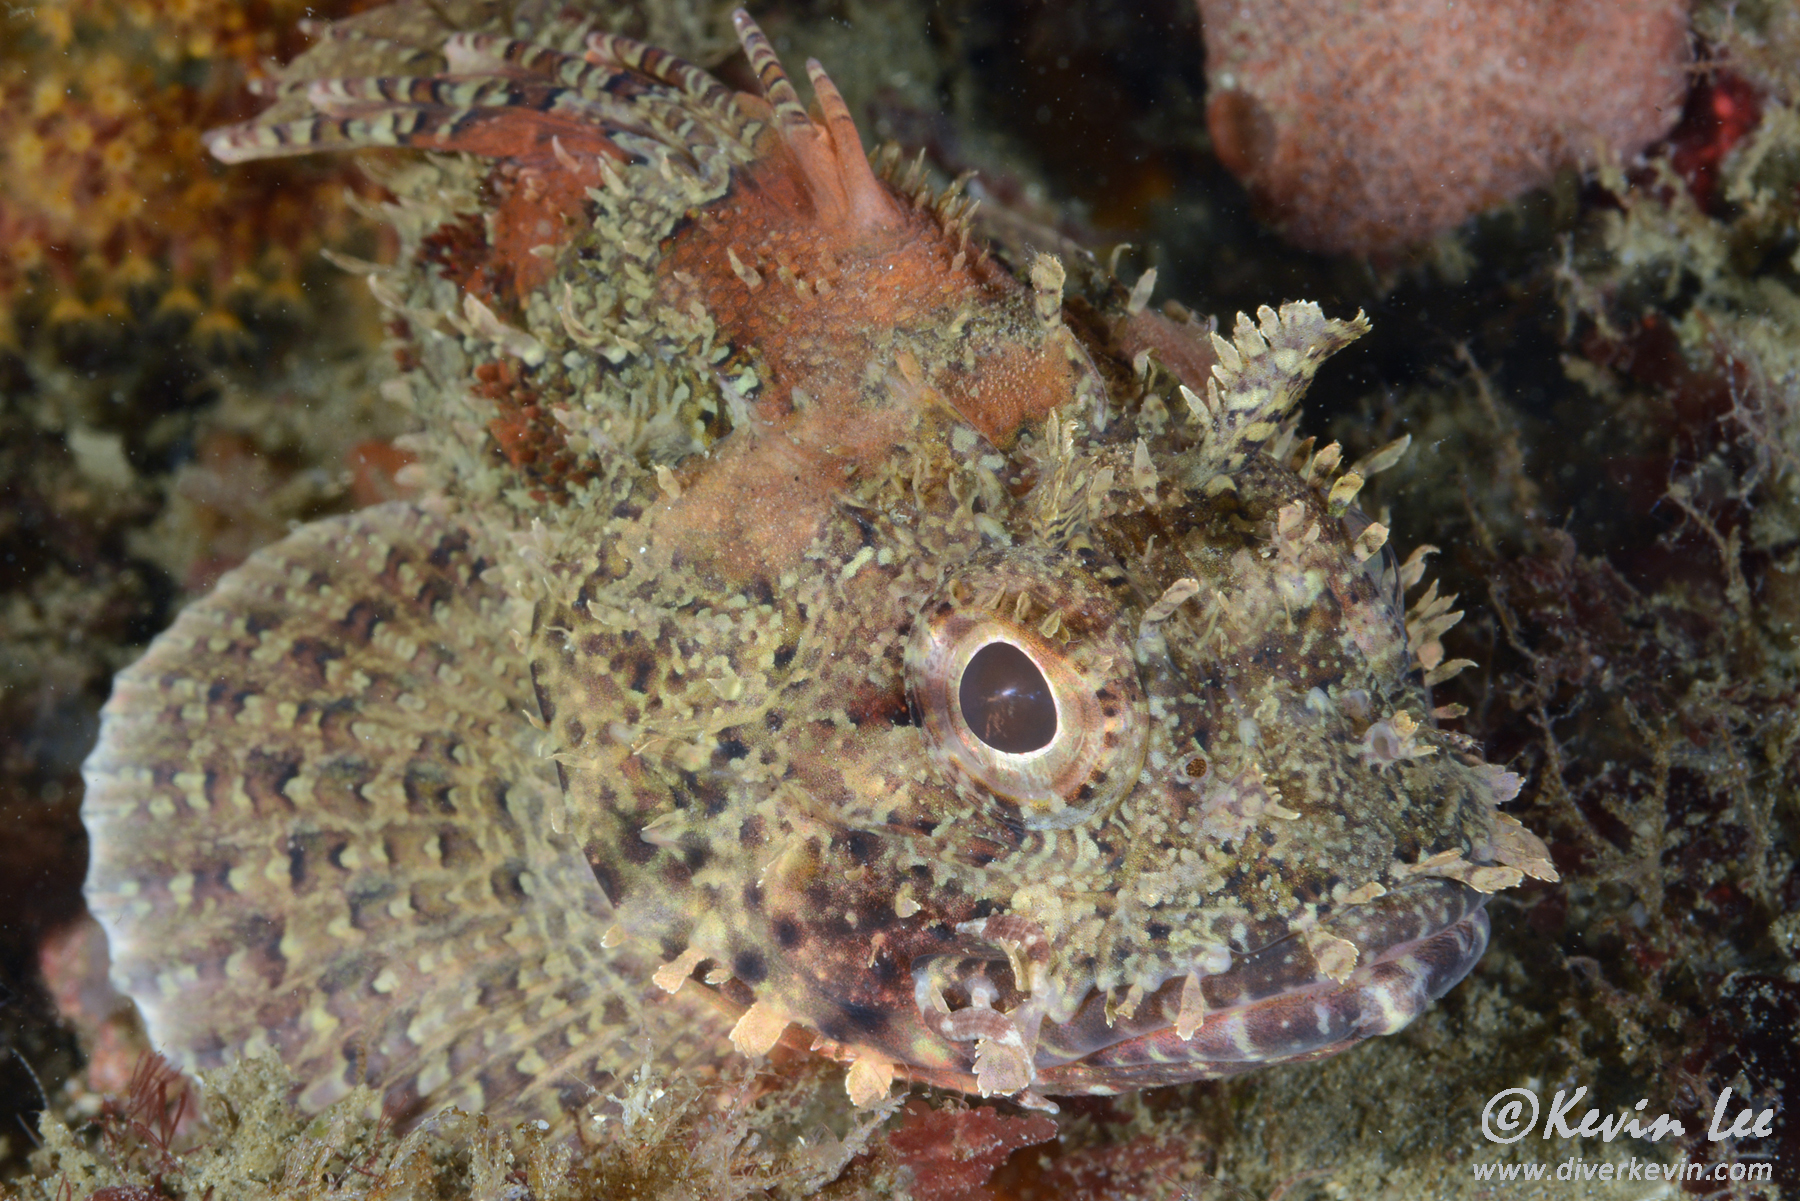
\includegraphics{cover_photo}~\\[1cm]
\pdftooltip{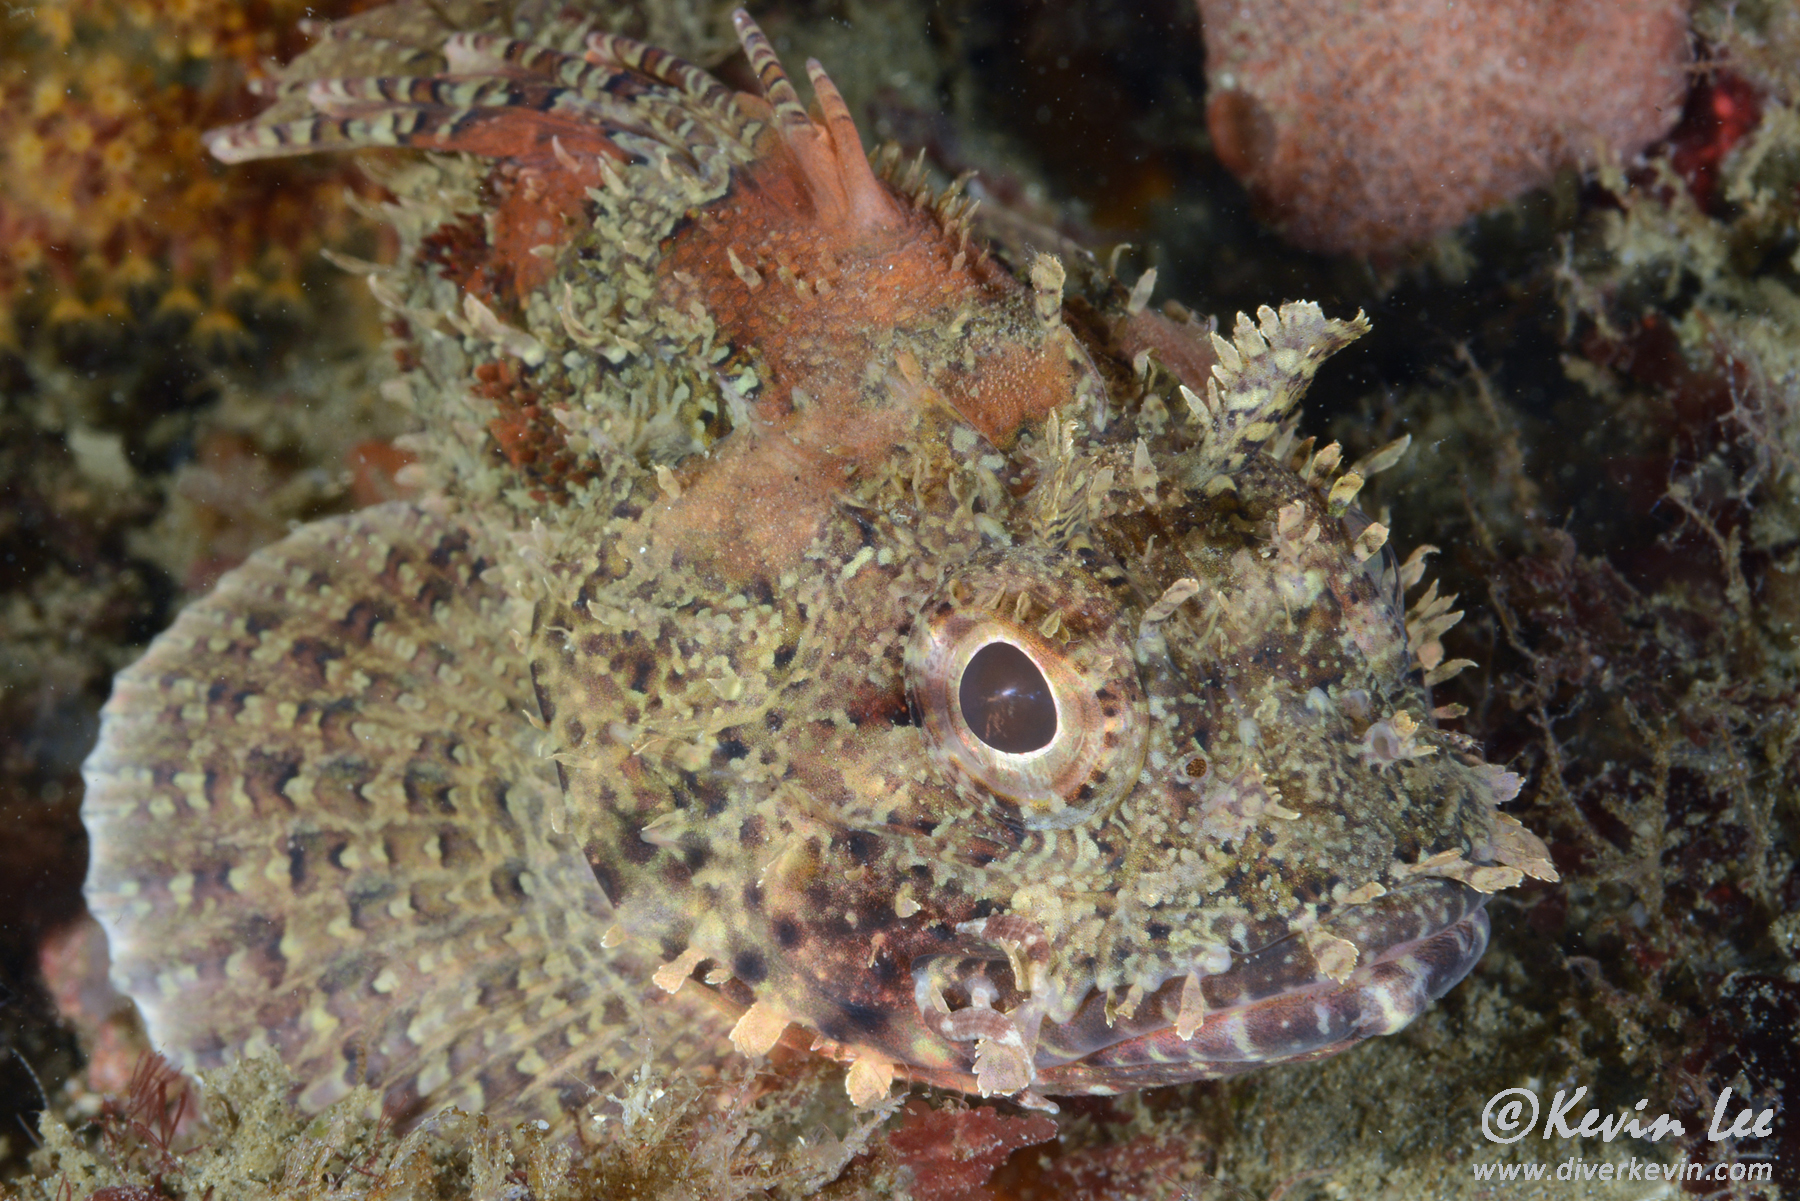
\includegraphics{cover_photo}}{This is a fish.}



Melissa H. Monk\textsuperscript{1}\\
Xi He\textsuperscript{1}\\
John Budrick\textsuperscript{2}\\

\vspace{.5cm}

\small
\textsuperscript{1}Southwest Fisheries Science Center, U.S. Department of Commerce, National Oceanic and Atmospheric Administration, National Marine Fisheries Service, 110 Shaffer Road, Santa Cruz, California 95060\\

\vspace{.3cm}

\textsuperscript{2}California Department of Fish and Wildlife, 350 Harbor Blvd., Belmont, California 94002\\


\vspace{.5cm}

\vfill
DRAFT SAFE\\
Disclaimer: This information is distributed solely for the purpose of pre-dissemination
peer review under applicable information quality guidelines. It has not been formally
disseminated by NOAA Fisheries. It does not represent and should not be construed to
represent any agency determination or policy. 

\vspace{.3cm}
%Bottom of the page
%{\large \today}

\maketitle

\pagenumbering{roman}
\setcounter{page}{1}
\end{center}

{
\setcounter{tocdepth}{4}
\tableofcontents
}
\setlength{\parskip}{5mm plus1mm minus1mm} \pagebreak

\pagenumbering{arabic} \setcounter{page}{1}
\renewcommand{\thefigure}{\alph{figure}}
\renewcommand{\thetable}{\alph{table}}

\section*{Executive Summary}\label{executive-summary}
\addcontentsline{toc}{section}{Executive Summary}

\subsection*{Stock}\label{stock}
\addcontentsline{toc}{subsection}{Stock}

This assessment reports the status of the California scorpionfish
(\emph{Scorpaena guttata}) resource in U.S. waters off the coast of the
California, Oregon, and Washington using data through 2016. Etc\ldots{}

\subsection*{Catches}\label{catches}
\addcontentsline{toc}{subsection}{Catches}

Catch figure(s) with fleets: (Figures
\ref{fig:Exec_catch1}-\ref{fig:Exec_catch3})\\
Catch table: (Table \ref{tab:Exec_catch})

\FloatBarrier

\begin{figure}[htbp]
\centering
\includegraphics{Assessment_template_files/figure-latex/unnamed-chunk-2-1.pdf}
\caption{California scorpionfish landings history for the recreational
fleets. \label{fig:Exec_catch1}}
\end{figure}

\begin{figure}[htbp]
\centering
\includegraphics{Assessment_template_files/figure-latex/unnamed-chunk-3-1.pdf}
\caption{Stacked line plot of California scorpionfish landings history
for the commercial fleets. \label{fig:Exec_catch2}}
\end{figure}

\begin{figure}[htbp]
\centering
\includegraphics{Assessment_template_files/figure-latex/unnamed-chunk-4-1.pdf}
\caption{Stacked line plot of California scorpionfish landings history
by region, north of Pt. Conception, between Pt. Conception and the
U.S.-Mexico border, and Mexican waters. \label{fig:Exec_catch3}}
\end{figure}

\FloatBarrier

\begin{figure}[htbp]
\centering
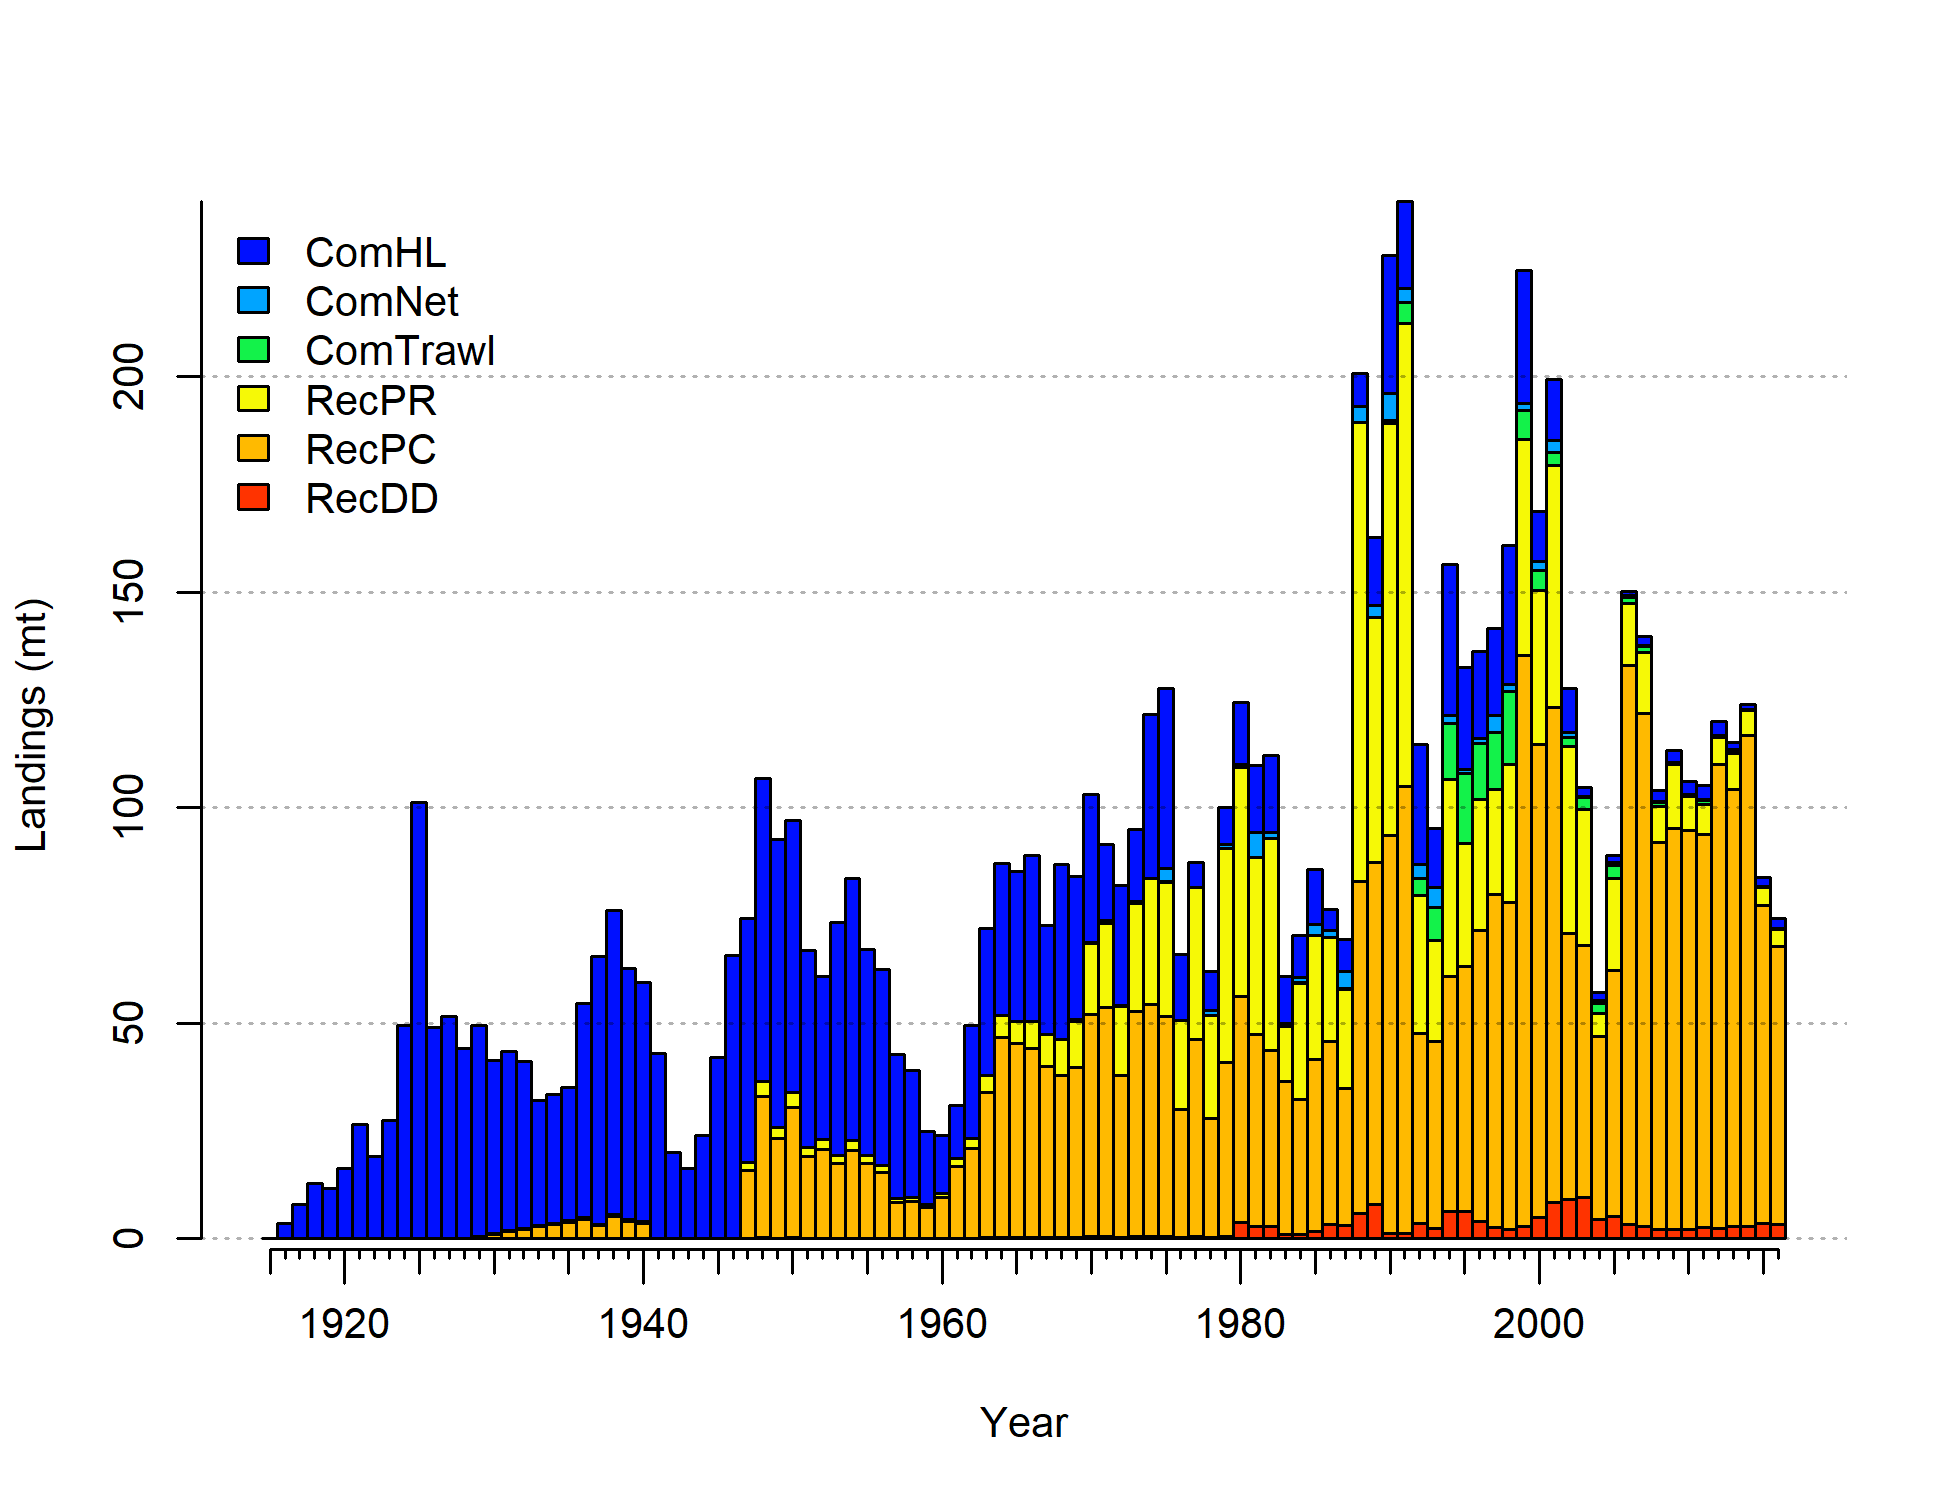
\includegraphics{r4ss/plots_mod1/catch2 landings stacked.png}
\caption{Landings history of California scorpionfish in the base model.
\label{fig:r4ss_catches}}
\end{figure}

\begin{table}[ht]
\centering
\caption{Recent California scorpionfish landings (mt) by 
                                            recreational (Rec.) and commercial (Com.) fleets.} 
\label{tab:Exec_catch}
\begin{tabular}{l>{\centering}p{.6in}>{\centering}p{1.1in}>{\centering}p{.9in}>{\centering}p{1.1in}>{\centering}p{.5in}>{\centering}p{.5in}>{\centering}p{.5in}}
  \hline
Year & Rec. Private & Rec. Party/Charter & Rec. Dead Discards & Com. Hook-and-line & Com. Trawl & Com. Gillnet & Total \\ 
  \hline
2007 & 14.24 & 118.87 & 2.89 & 1.90 & 1.48 & 0.21 & 139.58 \\ 
  2008 & 8.38 & 89.65 & 2.25 & 2.46 & 0.86 & 0.28 & 103.89 \\ 
  2009 & 14.68 & 93.16 & 2.09 & 2.97 & 0.27 & 0.13 & 113.31 \\ 
  2010 & 8.07 & 92.55 & 2.03 & 2.99 & 0.18 & 0.14 & 105.97 \\ 
  2011 & 6.84 & 91.18 & 2.66 & 3.24 & 1.05 & 0.24 & 105.21 \\ 
  2012 & 6.22 & 107.63 & 2.34 & 3.22 & 0.43 & 0.18 & 120.00 \\ 
  2013 & 8.18 & 101.31 & 2.94 & 1.73 & 0.83 & 0.14 & 115.14 \\ 
  2014 & 5.88 & 113.83 & 2.93 & 1.03 & 0.13 & 0.04 & 123.82 \\ 
  2015 & 4.15 & 73.78 & 3.59 & 2.21 & 0.13 & 0.03 & 83.89 \\ 
  2016 & 3.86 & 64.56 & 3.29 & 2.32 & 0.13 & 0.00 & 74.16 \\ 
   \hline
\end{tabular}
\end{table}

\FloatBarrier

\newpage

\subsection*{Data and Assessment}\label{data-and-assessment}
\addcontentsline{toc}{subsection}{Data and Assessment}

California scorpionfish was assessed in 2005 (Maunder et al.
\protect\hyperlink{ref-Maunder2005}{2005}) using Stock Synthesis II
version 1.18. This assessment uses the newest version of Stock Synthesis
(3.30.0.4). The model begins in 1916, and assumes the stock was at an
unfished equilibrium that year.

Map of assessment region: (Figure \ref{fig:assess_region_map}).

\begin{figure}[htbp]
\centering
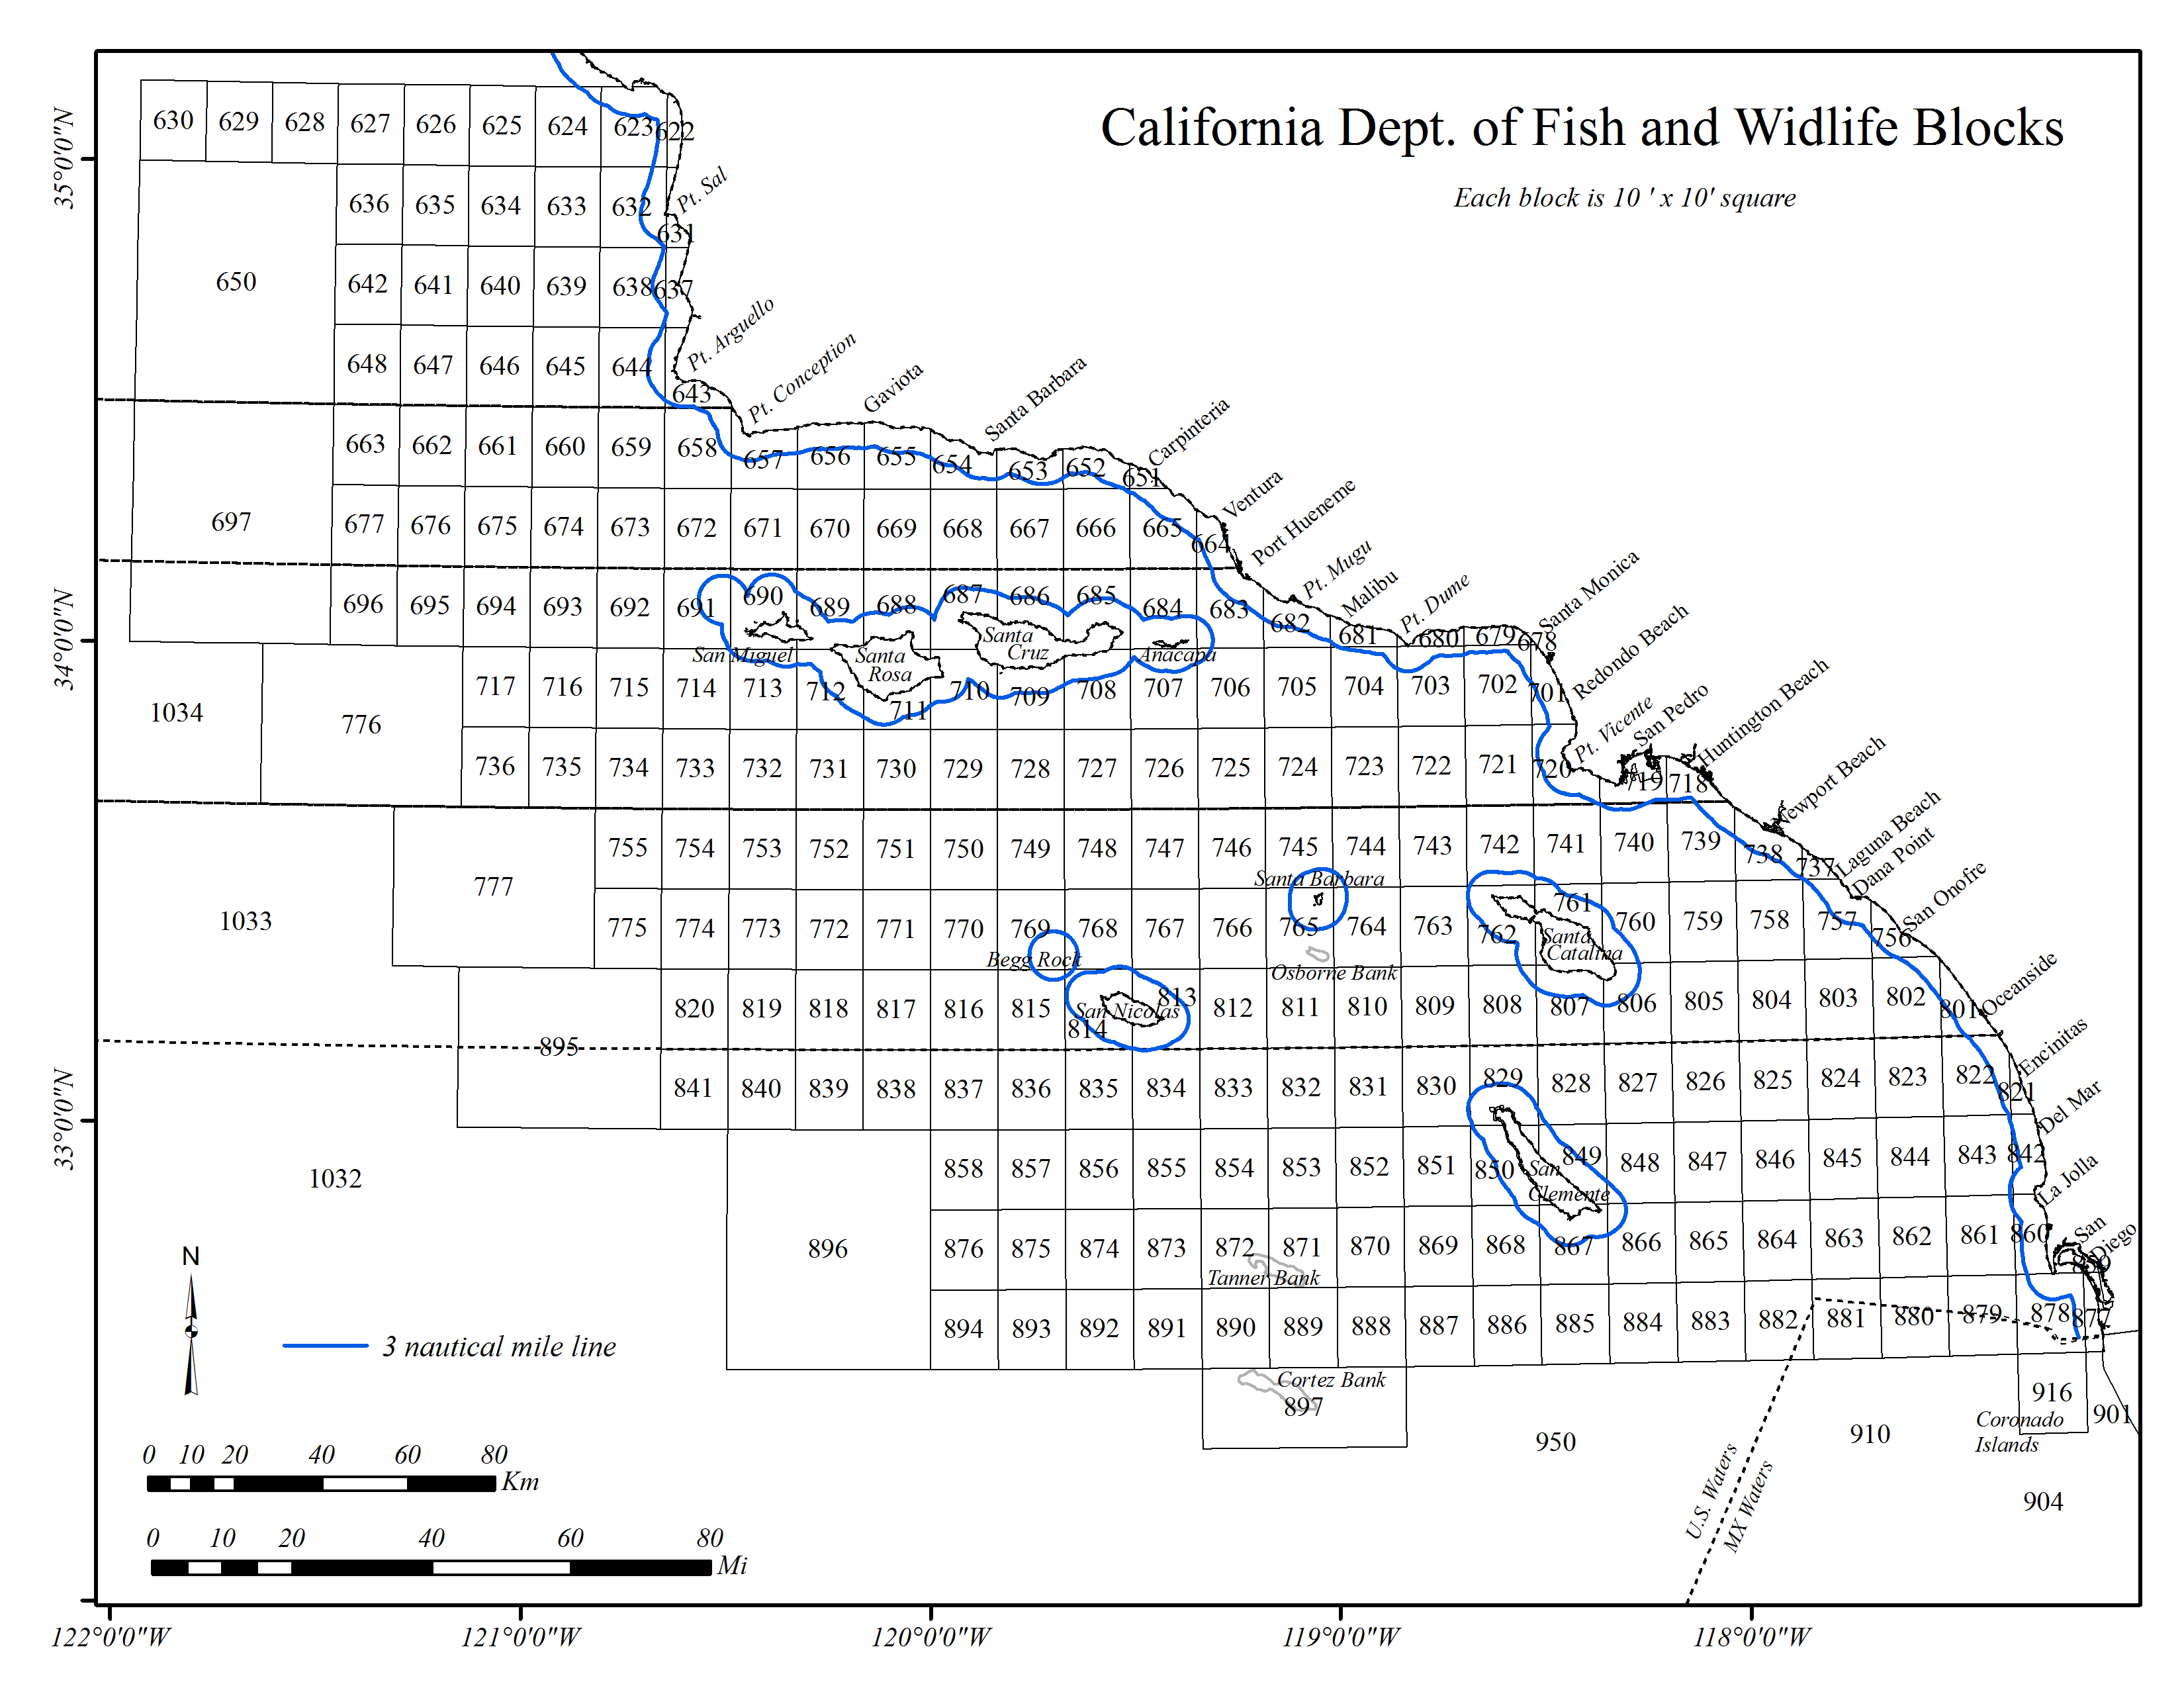
\includegraphics{Figures/assess_region_map.png}
\caption{Map depicting the boundaries for the base-case model.
\label{fig:assess_region_map}}
\end{figure}

\FloatBarrier

\subsection*{Stock Biomass}\label{stock-biomass}
\addcontentsline{toc}{subsection}{Stock Biomass}

Spawning output Figure: Figure \ref{fig:Spawnbio_all}\\
Spawning output Table(s): Table \ref{tab:SpawningDeplete_mod1}\\
Relative depletion Figure: Figure \ref{fig:RelDeplete_all}

The estimated relative depletion level (spawning output relative to
unfished spawning output) of the the base-case model in 2016 is 70.4\%
(\textasciitilde{}95\% asymptotic interval: \(\pm\) 53.8\%-87\%) (Figure
\ref{fig:RelDeplete_all}).

\FloatBarrier

\begin{table}[ht]
\centering
\caption{Recent trend in beginning of the 
                                      year spawning output and depletion for
                                      the base model for California scorpionfish.} 
\label{tab:SpawningDeplete_mod1}
\begin{tabular}{l>{\centering}p{1.3in}>{\centering}p{1.2in}>{\centering}p{1in}>{\centering}p{1.2in}}
  \hline
Year & Spawning Output (mt) & \~{} 95\% confidence interval & Estimated depletion & \~{} 95\% confidence interval \\ 
  \hline
2008 & 1411.880 & (826-1997.76) & 0.821 & (0.667-0.976) \\ 
  2009 & 1327.280 & (779.49-1875.07) & 0.772 & (0.628-0.916) \\ 
  2010 & 1240.230 & (727.54-1752.92) & 0.722 & (0.587-0.856) \\ 
  2011 & 1188.880 & (694.44-1683.32) & 0.692 & (0.561-0.823) \\ 
  2012 & 1180.620 & (686.04-1675.2) & 0.687 & (0.556-0.818) \\ 
  2013 & 1149.250 & (662.71-1635.79) & 0.669 & (0.541-0.796) \\ 
  2014 & 1103.550 & (630.12-1576.98) & 0.642 & (0.517-0.767) \\ 
  2015 & 1085.150 & (607.15-1563.15) & 0.631 & (0.504-0.759) \\ 
  2016 & 1122.560 & (616.11-1629.01) & 0.653 & (0.516-0.79) \\ 
  2017 & 1209.890 & (634.69-1785.09) & 0.704 & (0.538-0.87) \\ 
   \hline
\end{tabular}
\end{table}

\FloatBarrier

\begin{figure}[htbp]
\centering
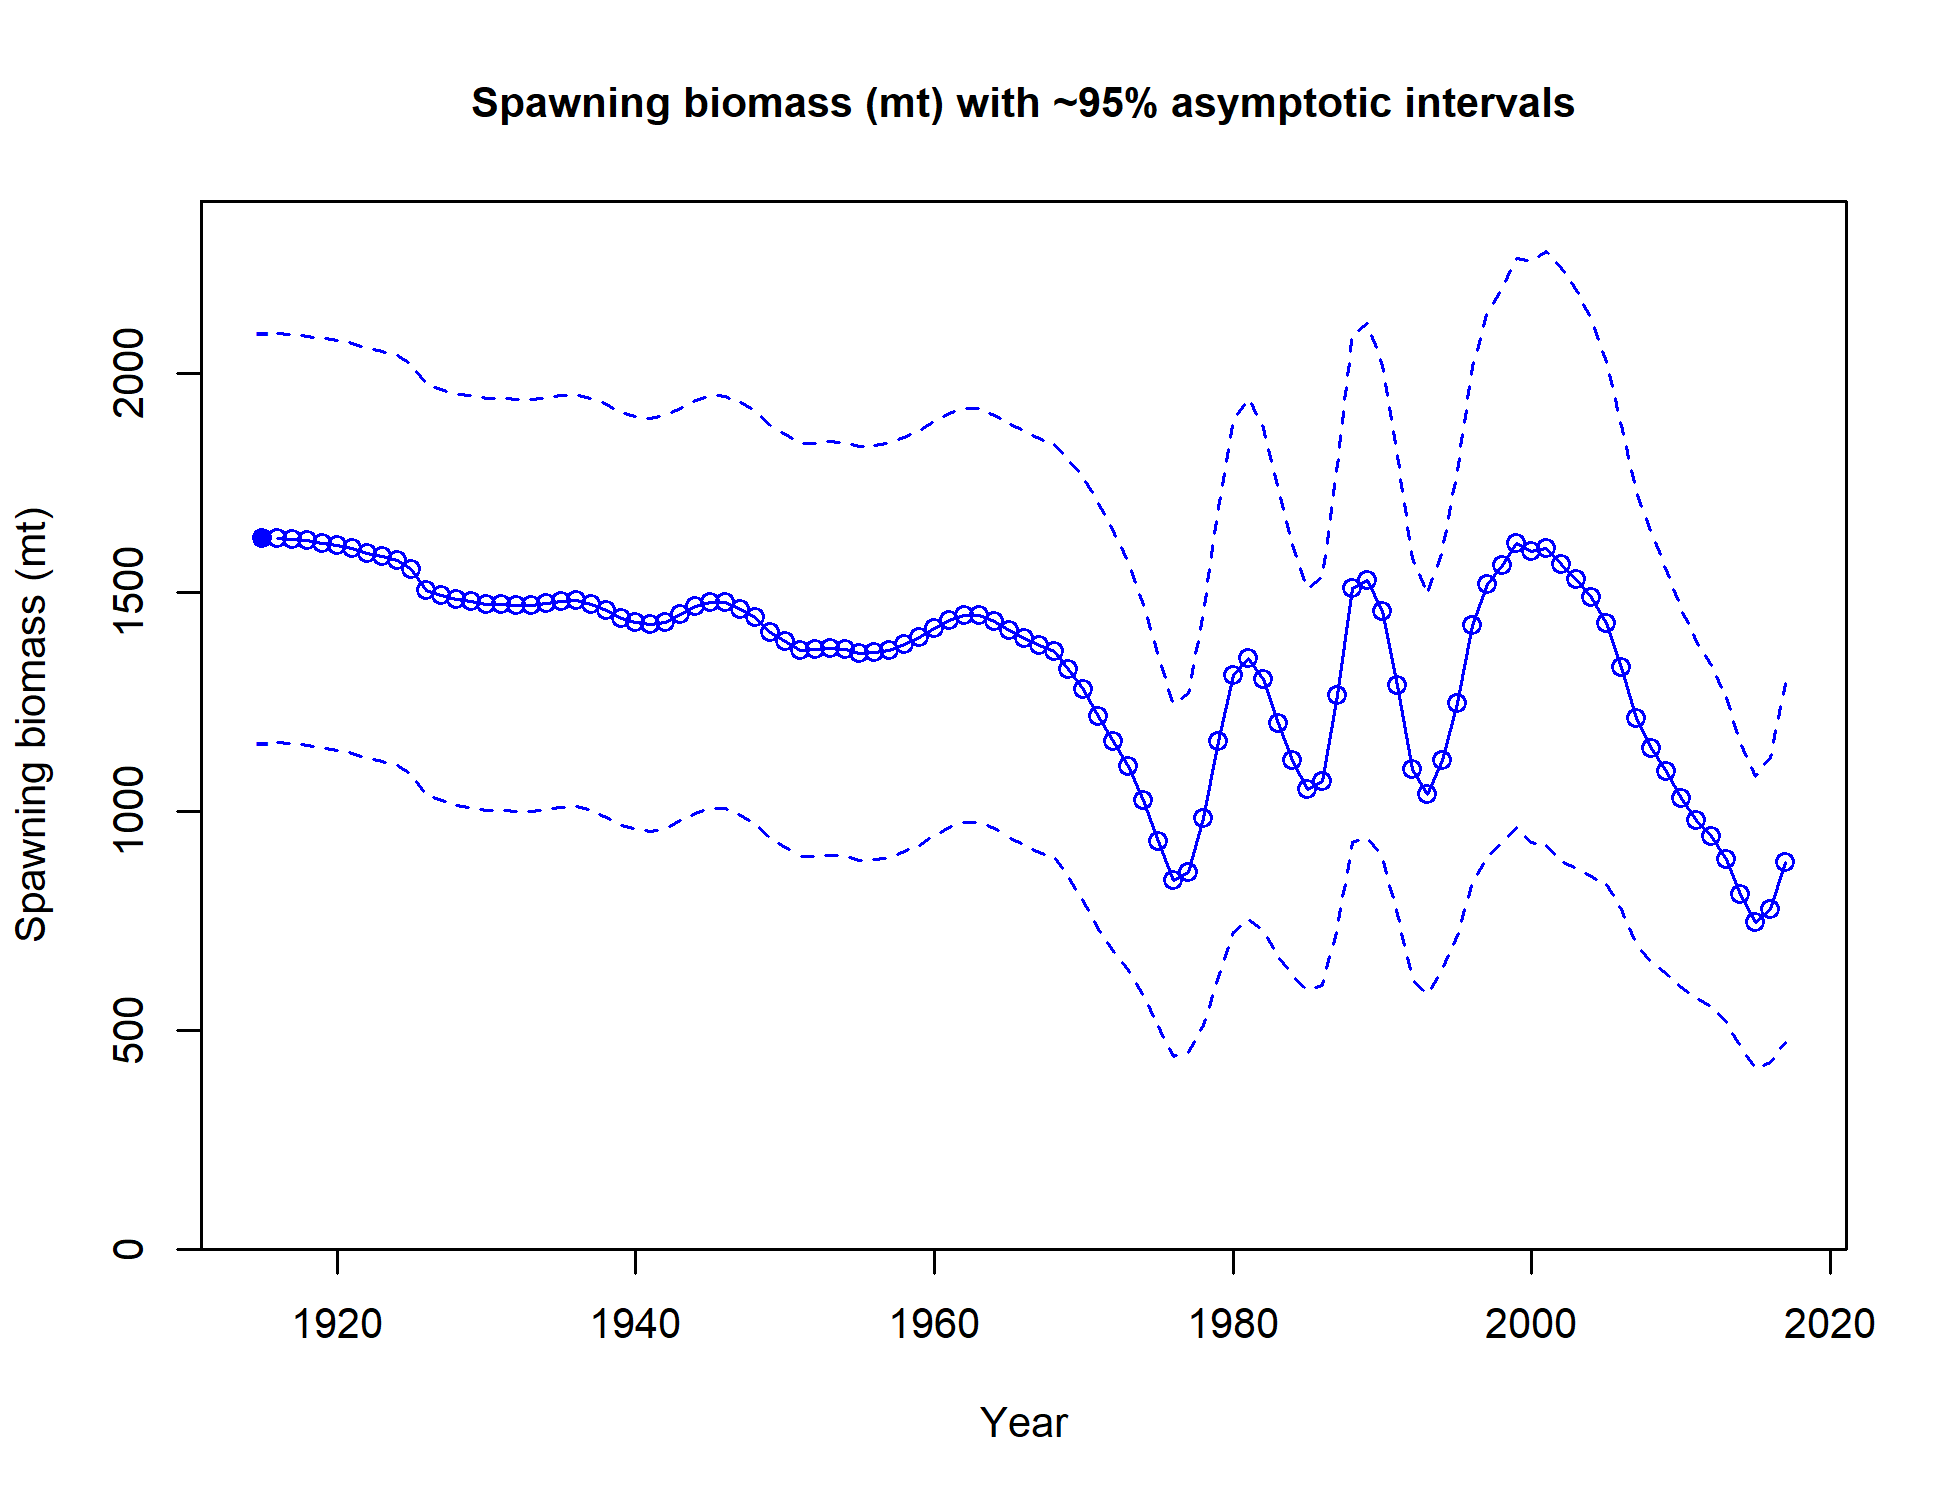
\includegraphics{r4ss/plots_mod1/ts7_Spawning_biomass_(mt)_with_95_asymptotic_intervals_intervals.png}
\caption{Time series of spawning output trajectory (circles and line:
median; light broken lines: 95\% credibility intervals) for the base
case assessment model. \label{fig:Spawnbio_all}}
\end{figure}

\begin{figure}[htbp]
\centering
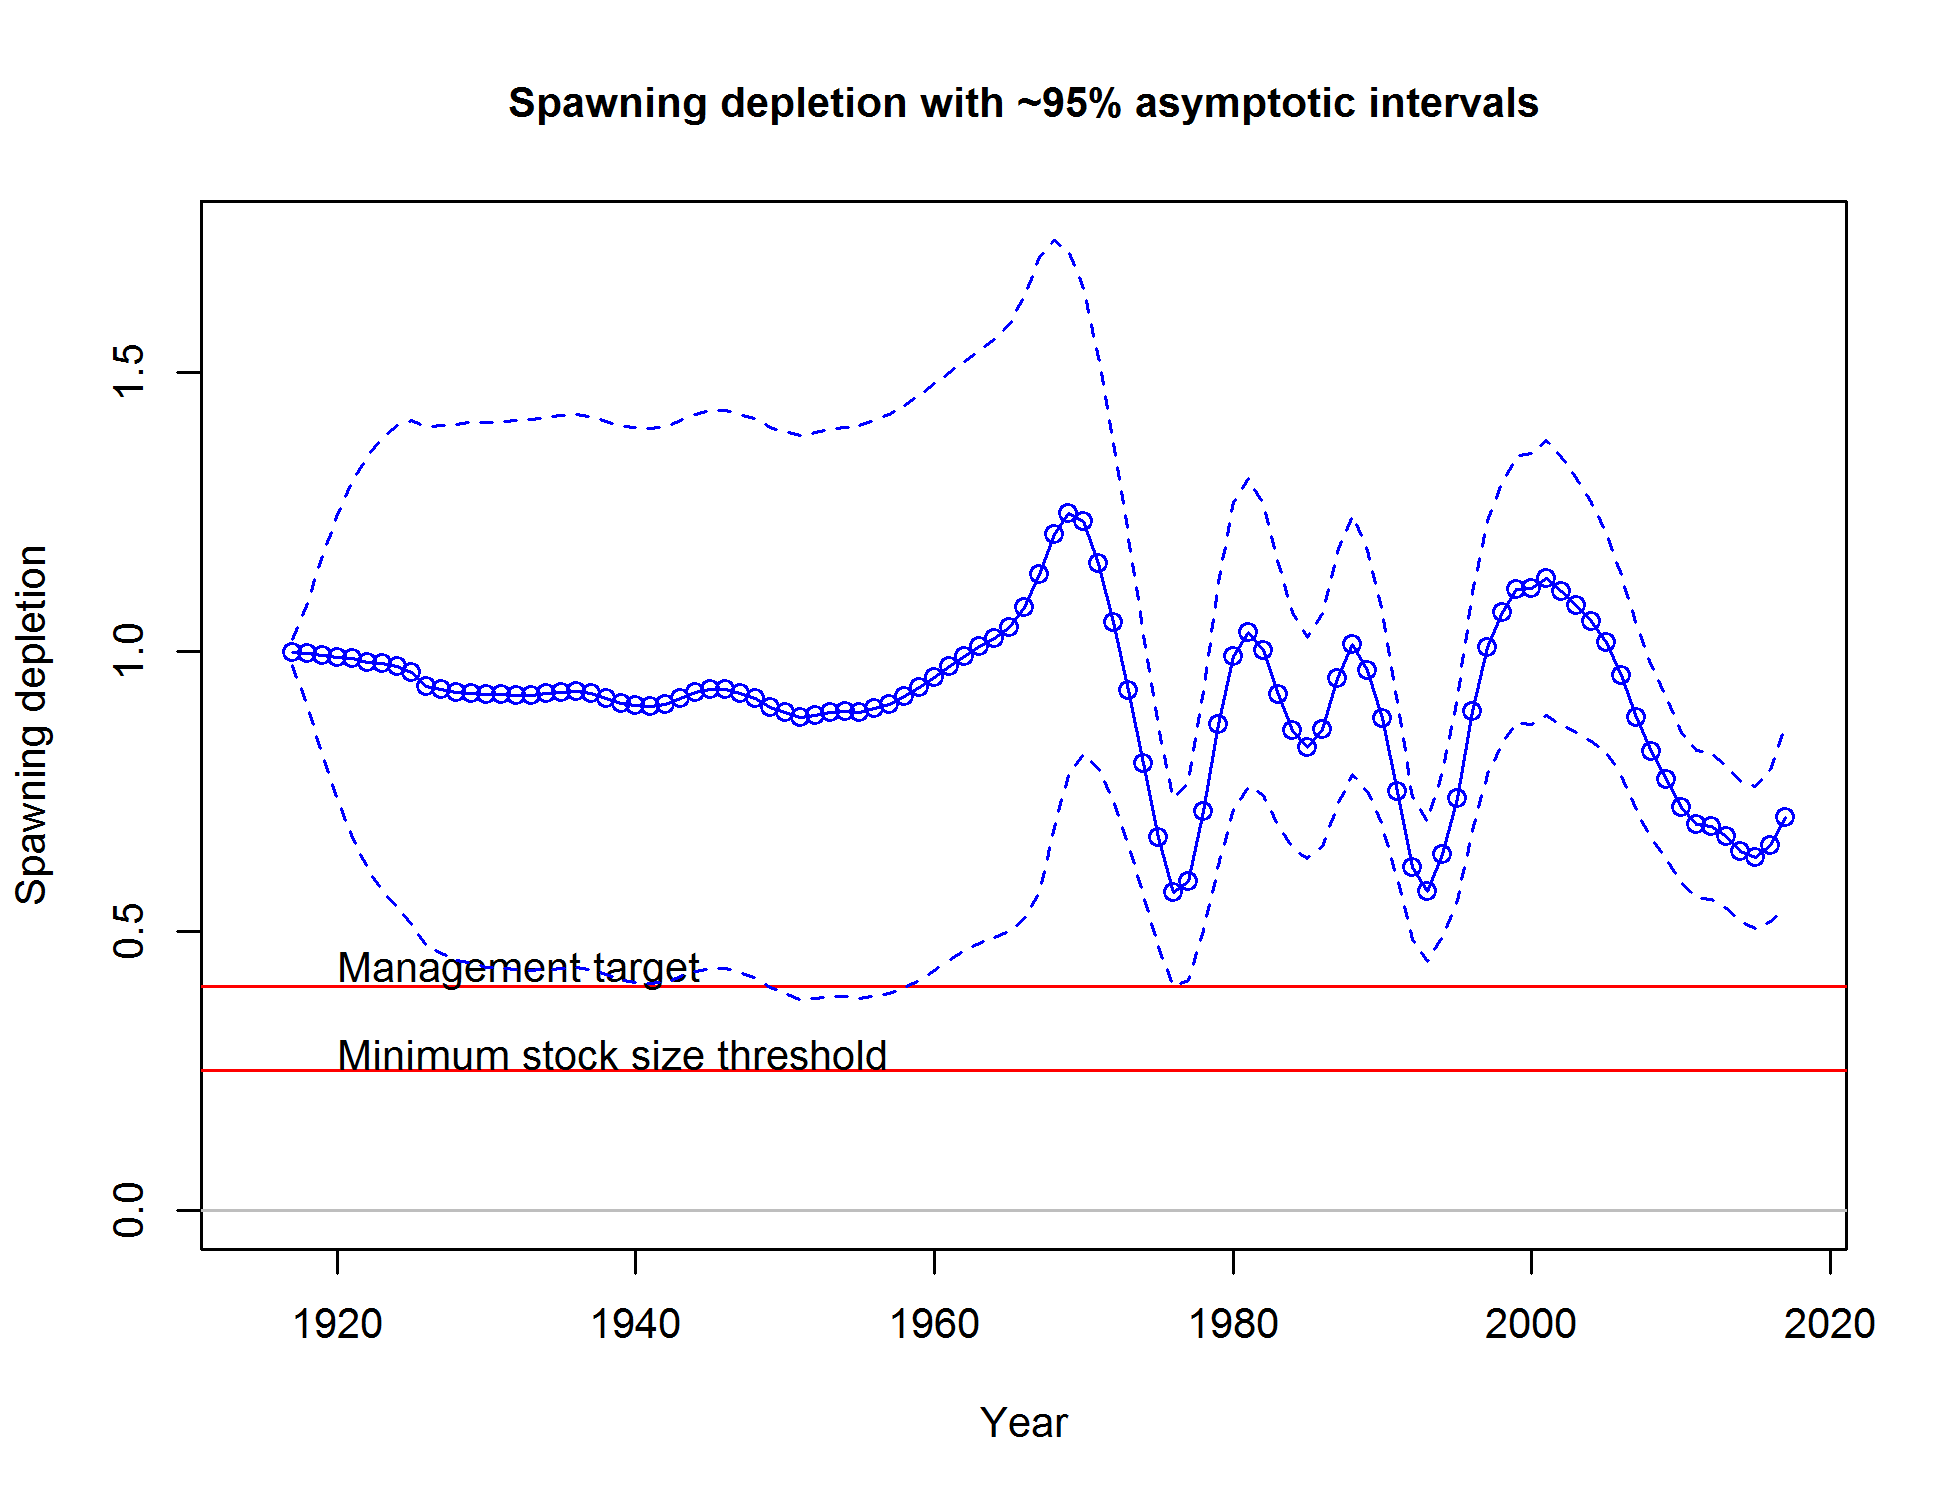
\includegraphics{r4ss/plots_mod1/ts9_Spawning_depletion_with_95_asymptotic_intervals_intervals.png}
\caption{Estimated relative depletion with approximate 95\% asymptotic
confidnce intervals (dashed lines) for the base case assessment model.
\label{fig:RelDeplete_all}}
\end{figure}

\FloatBarrier

\subsection*{Recruitment}\label{recruitment}
\addcontentsline{toc}{subsection}{Recruitment}

Recruitment Figure: (Figure \ref{fig:Recruits_all})\\
Recruitment Tables: (Tables \ref{tab:Recruit_mod1},
\ref{tab:Recruit_mod2} and \ref{tab:Recruit_mod3})

\begin{table}[ht]
\centering
\caption{Recent recruitment for the base model.} 
\label{tab:Recruit_mod1}
\begin{tabular}{>{\centering}p{.8in}>{\centering}p{1.6in}>{\centering}p{1.3in}}
  \hline
Year & Estimated Recruitment (1,000s) & \~{} 95\% confidence interval \\ 
  \hline
2008 & 2334.67 & (1188.11 - 4587.71) \\ 
  2009 & 3043.29 & (1586.6 - 5837.4) \\ 
  2010 & 5924.02 & (3274.03 - 10718.9) \\ 
  2011 & 1919.20 & (814.17 - 4524.02) \\ 
  2012 & 466.56 & (145.49 - 1496.19) \\ 
  2013 & 6221.57 & (3237.03 - 11957.84) \\ 
  2014 & 2427.69 & (894.39 - 6589.64) \\ 
  2015 & 7513.87 & (2659.09 - 21232.2) \\ 
  2016 & 3822.13 & (796 - 18352.62) \\ 
  2017 & 3861.95 & (804.12 - 18547.73) \\ 
   \hline
\end{tabular}
\end{table}

\FloatBarrier

\begin{figure}[htbp]
\centering
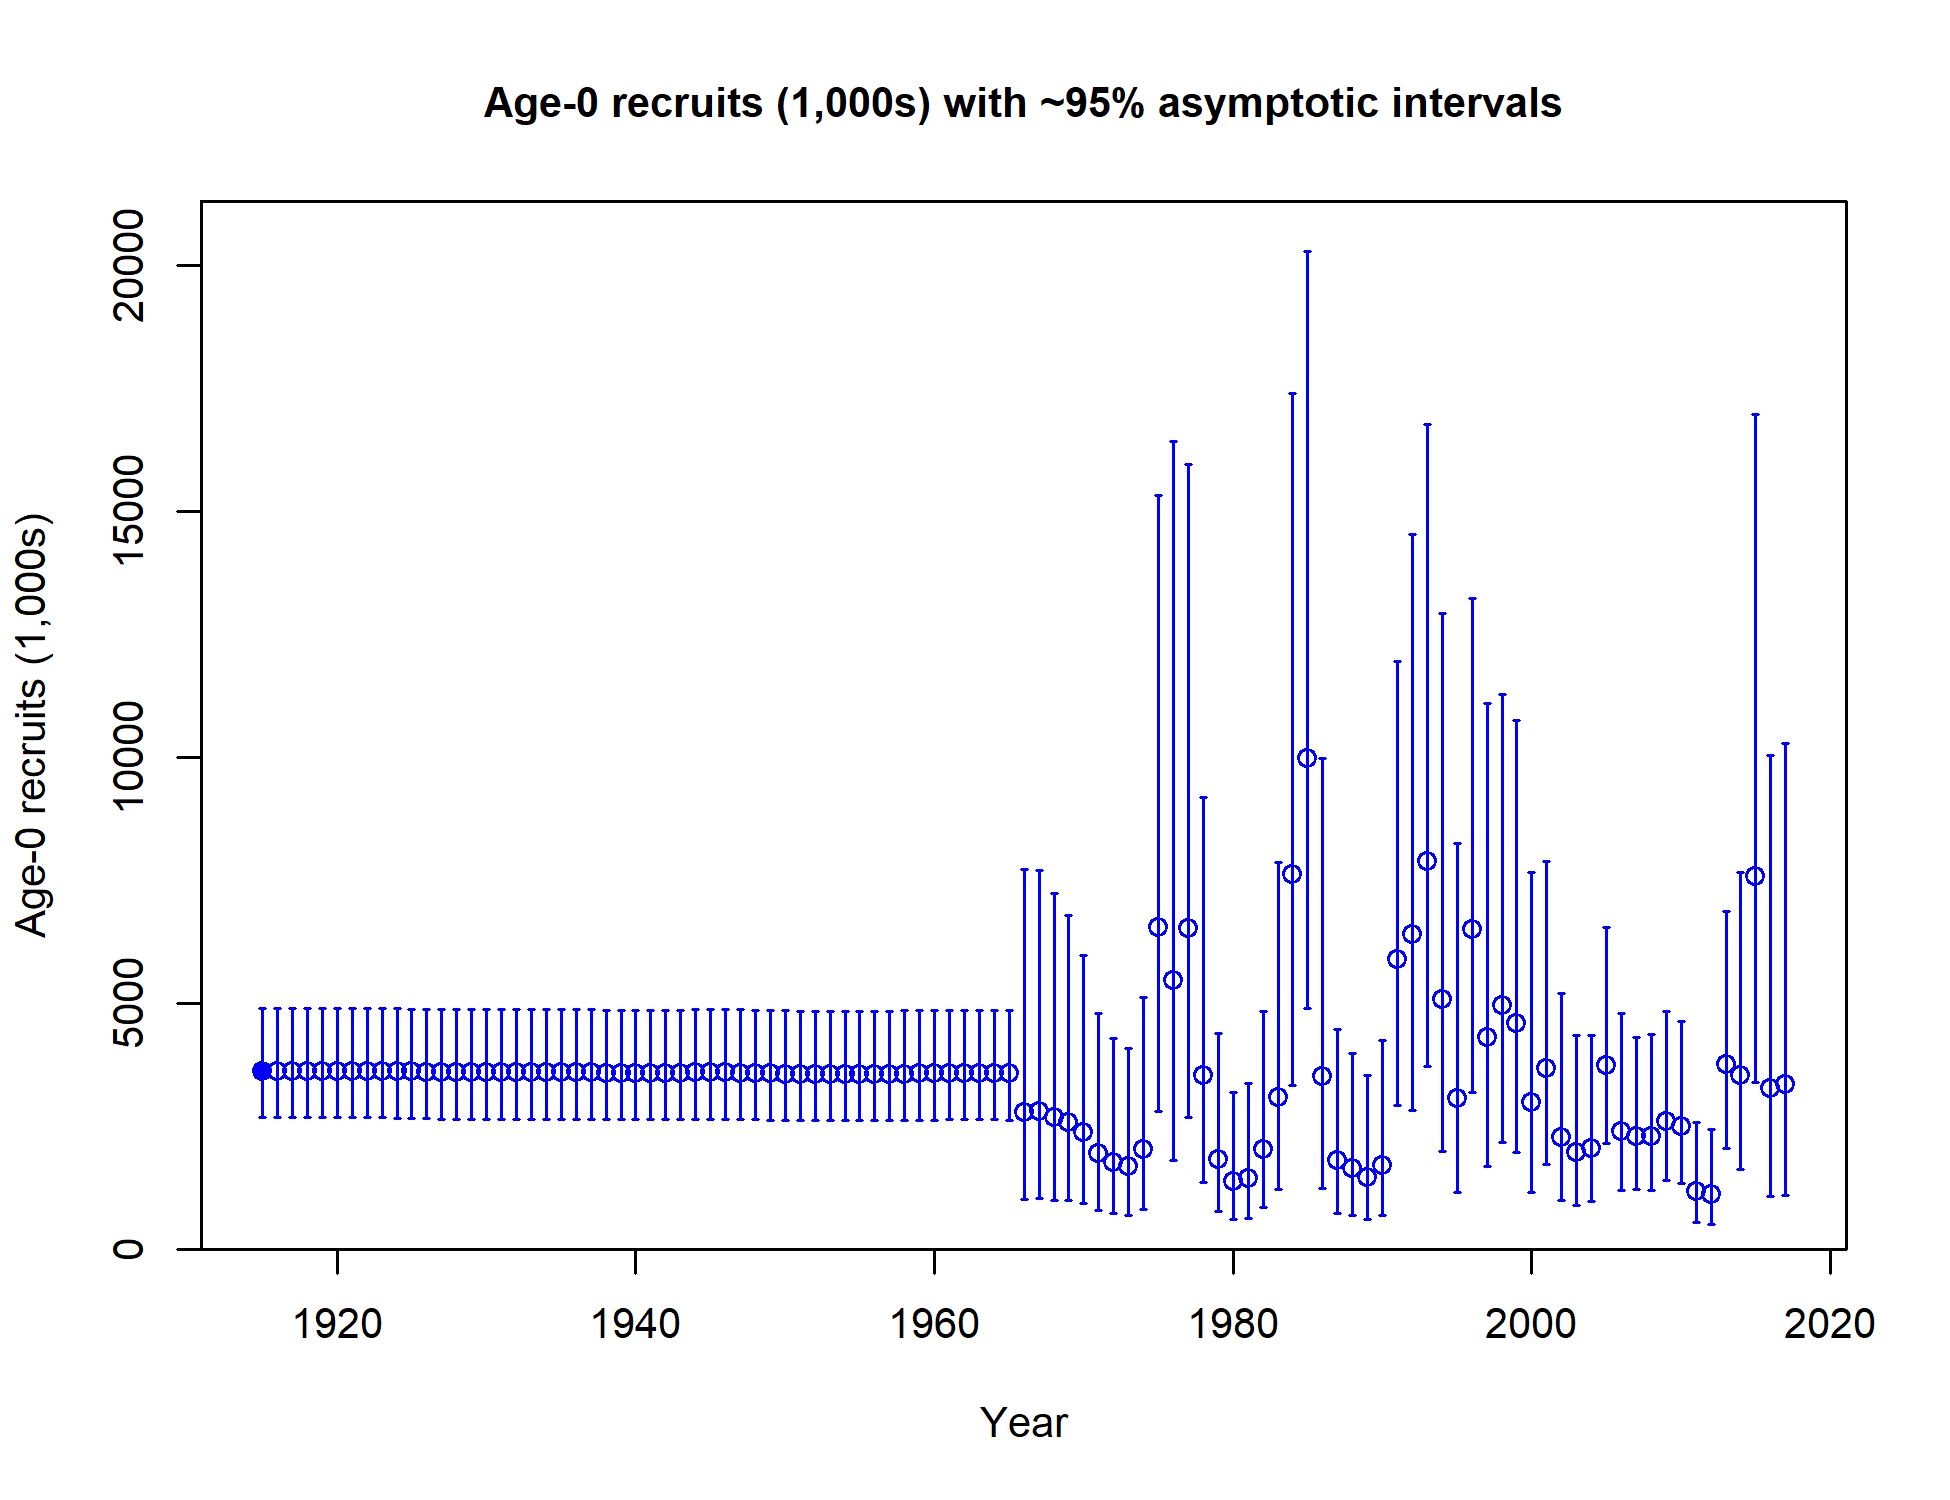
\includegraphics{r4ss/plots_mod1/ts11_Age-0_recruits_(1000s)_with_95_asymptotic_intervals.png}
\caption{Time series of estimated California scorpionfish recruitments
for the base-case model with 95\% confidence or credibility intervals.
\label{fig:Recruits_all}}
\end{figure}

\FloatBarrier

\subsection*{Exploitation status}\label{exploitation-status}
\addcontentsline{toc}{subsection}{Exploitation status}

Exploitation Tables: Table \ref{tab:SPR_Exploit_mod1}, Table
\ref{tab:SPR_Exploit_mod2}, Table \ref{tab:SPR_Exploit_mod3}
Exploitation Figure: Figure \ref{fig:SPR_all}).

A summary of California scorpionfish exploitation histories for base
model is provided as Figure \ref{fig:Phase_all}.

\FloatBarrier

\begin{table}[ht]
\centering
\caption{Recent trend in spawning potential 
                                        ratio and exploitation for California scorpionfish in the base model.  Fishing intensity is (1-SPR) 
                                        divided by 50\% (the SPR target) and exploitation 
                                        is F divided by F\textsubscript{SPR}.} 
\label{tab:SPR_Exploit_mod1}
\begin{tabular}{l>{\centering}p{1in}>{\centering}p{1.2in}>{\centering}p{1in}>{\centering}p{1.2in}}
  \hline
Year & Fishing intensity & \~{} 95\% confidence interval & Exploitation rate & \~{} 95\% confidence interval \\ 
  \hline
2007 & 0.36 & (0.21-0.52) & 0.04 & (0.02-0.06) \\ 
  2008 & 0.31 & (0.17-0.45) & 0.03 & (0.02-0.04) \\ 
  2009 & 0.34 & (0.19-0.5) & 0.04 & (0.02-0.05) \\ 
  2010 & 0.34 & (0.19-0.49) & 0.04 & (0.02-0.05) \\ 
  2011 & 0.36 & (0.2-0.51) & 0.03 & (0.02-0.05) \\ 
  2012 & 0.41 & (0.24-0.58) & 0.04 & (0.02-0.06) \\ 
  2013 & 0.41 & (0.24-0.59) & 0.04 & (0.02-0.06) \\ 
  2014 & 0.45 & (0.26-0.63) & 0.05 & (0.02-0.07) \\ 
  2015 & 0.35 & (0.19-0.51) & 0.03 & (0.02-0.05) \\ 
  2016 & 0.32 & (0.17-0.46) & 0.02 & (0.01-0.04) \\ 
   \hline
\end{tabular}
\end{table}

\FloatBarrier

\begin{figure}[htbp]
\centering
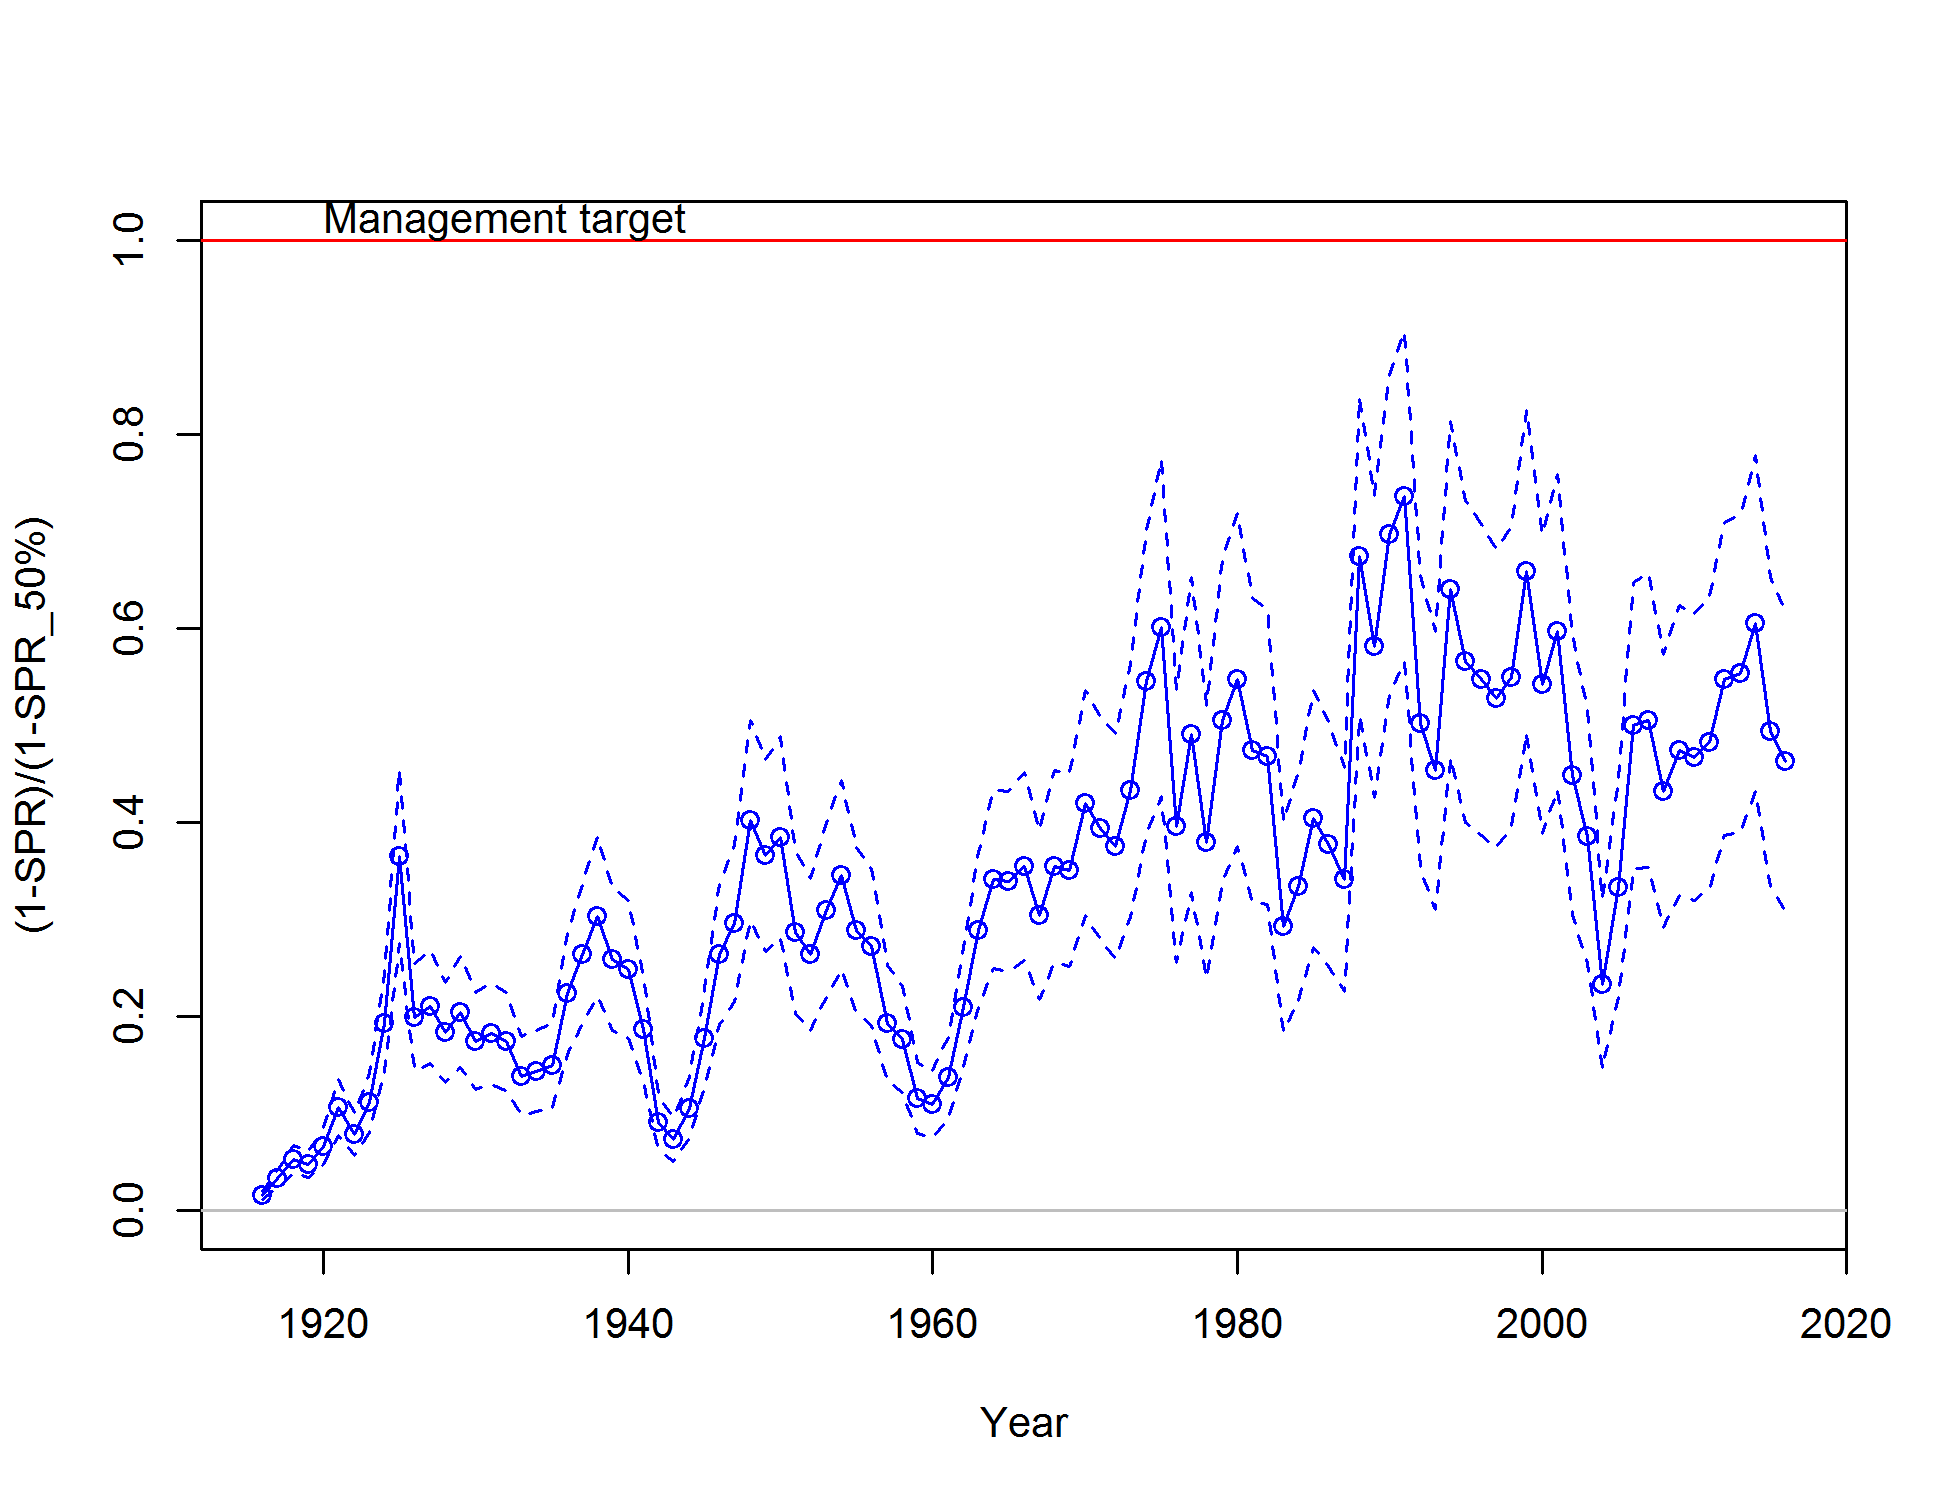
\includegraphics{r4ss/plots_mod1/SPR3_ratiointerval.png}
\caption{Estimated spawning potential ratio (SPR) for the base-case
model. One minus SPR is plotted so that higher exploitation rates occur
on the upper portion of the y-axis. The management target is plotted as
a red horizontal line and values above this reflect harvests in excess
of the overfishing proxy based on the SPR\textsubscript{50\%} harvest
rate. The last year in the time series is 2016. \label{fig:SPR_all}}
\end{figure}

\begin{figure}[htbp]
\centering
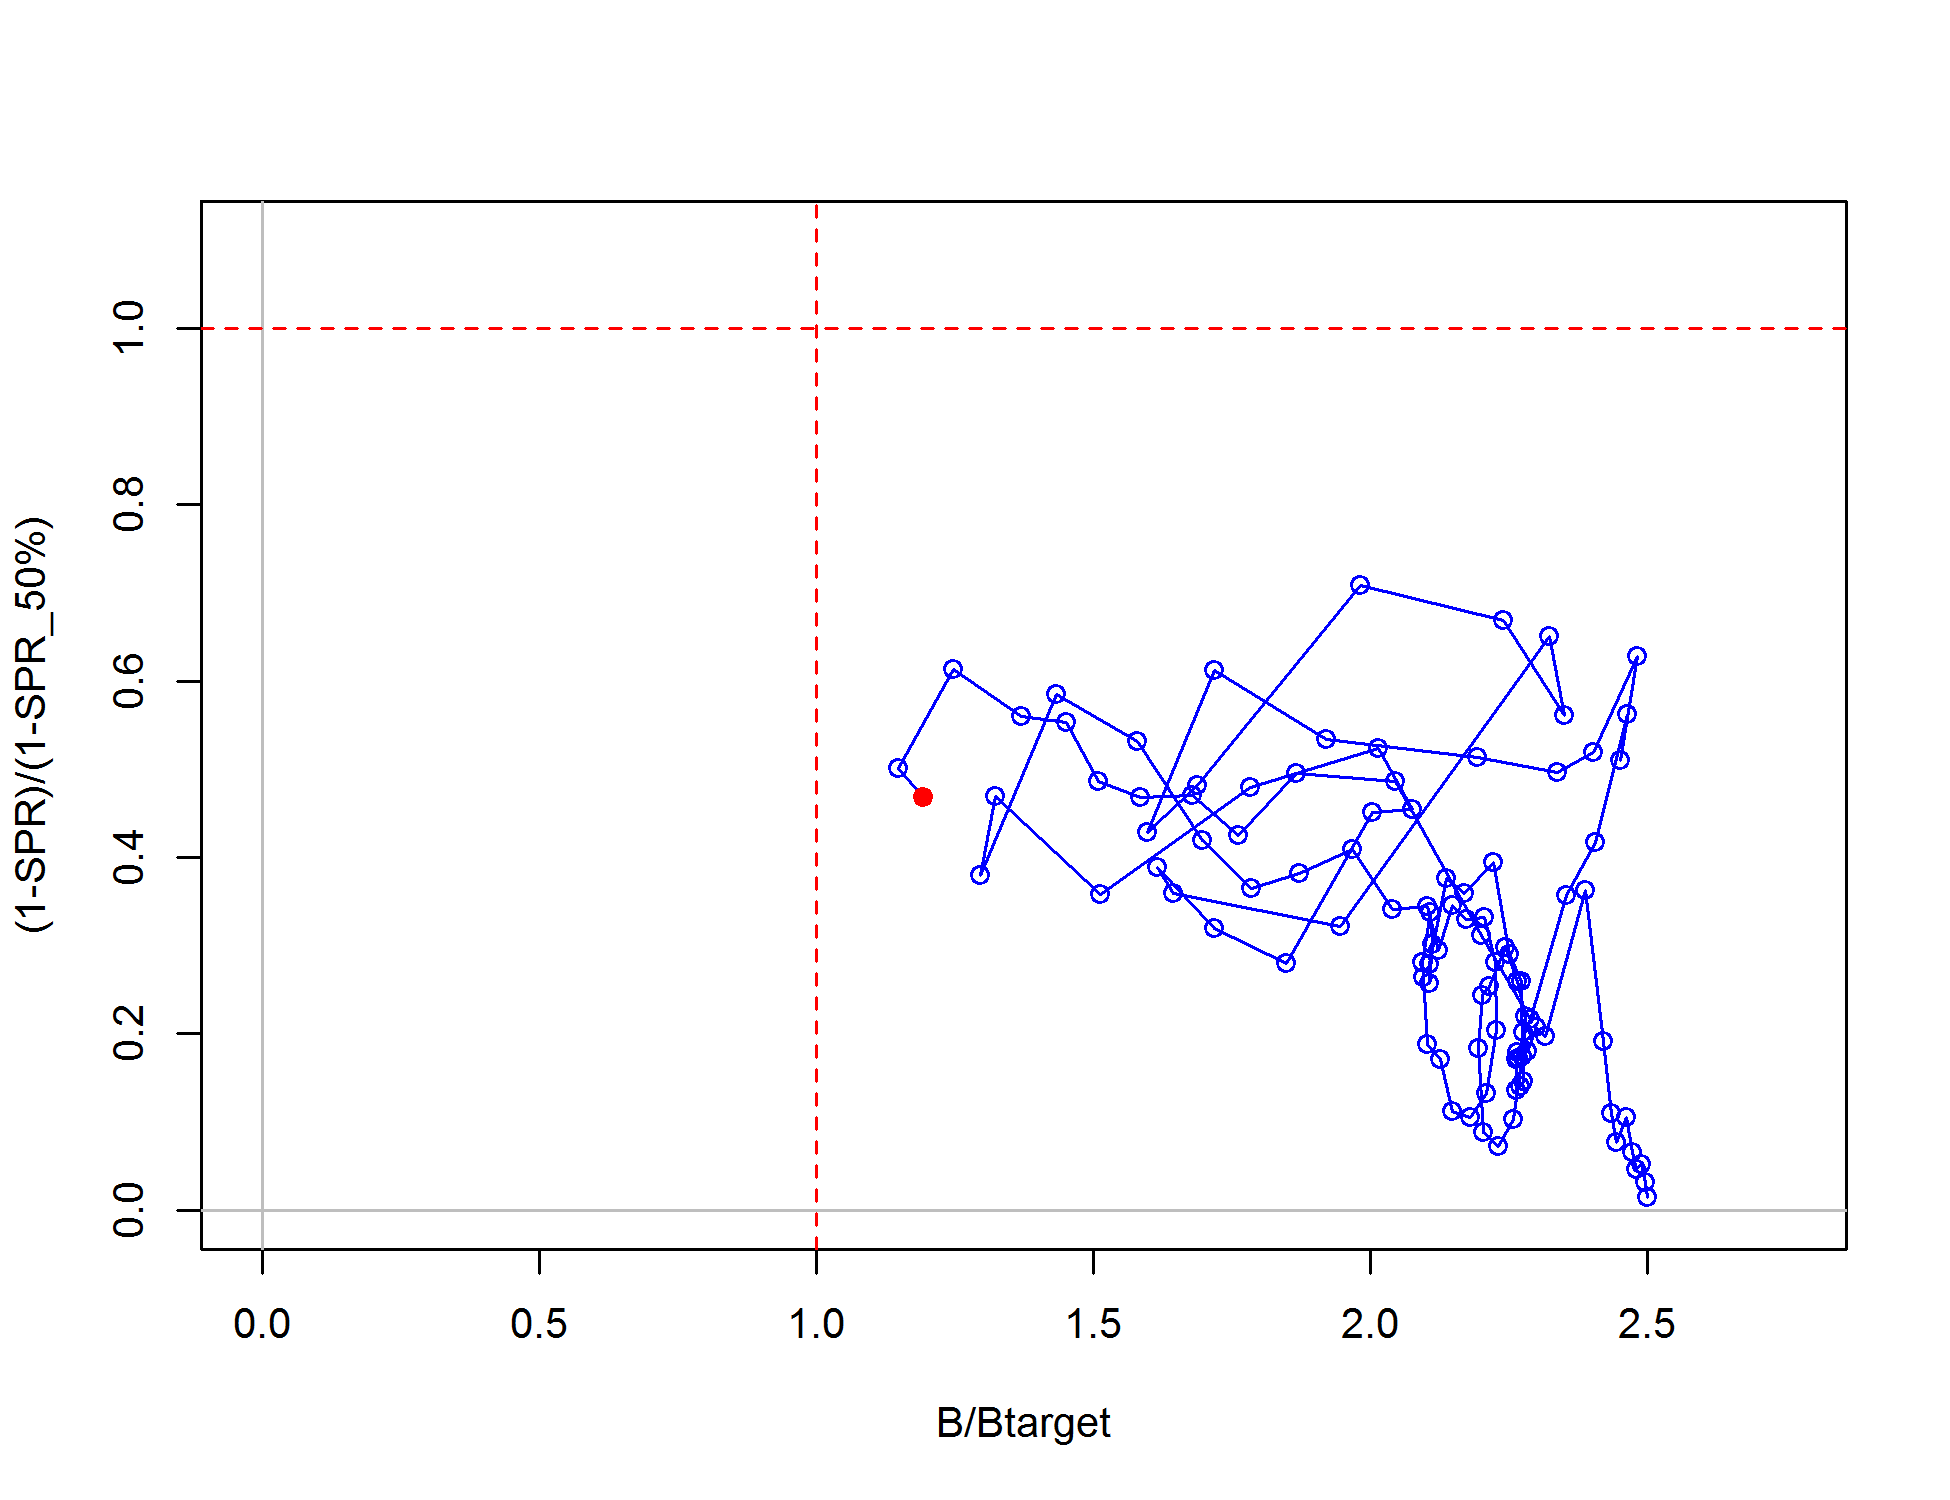
\includegraphics{r4ss/plots_mod1/SPR4_phase.png}
\caption{Phase plot of estimated relative (1-SPR) vs.~relative spawning
biomass for the base case model. The relative (1-SPR) is (1-SPR) divided
by 50\% (the SPR target). Relative depletion is the annual spawning
biomass divided by the unfished spawning biomass. \label{fig:Phase_all}}
\end{figure}

\FloatBarrier

\subsection*{Ecosystem Considerations}\label{ecosystem-considerations}
\addcontentsline{toc}{subsection}{Ecosystem Considerations}

In this assessment, ecosystem considerations were\ldots{}..

\subsection*{Reference Points}\label{reference-points}
\addcontentsline{toc}{subsection}{Reference Points}

This stock assessment estimates that California scorpionfish in the base
model are above the biomass target, but above the minimum stock size
threshold. \hl{Add sentence about spawning output trend.} The estimated
relative depletion level for \hl{Model 1} in 2016 is 70.4\%
(\textasciitilde{}95\% asymptotic interval: \(\pm\) 53.8\%-87\%,
corresponding to an unfished spawning output of 1209.89 mt
(\textasciitilde{}95\% asymptotic interval: 634.69-1785.09 mt) of
spawning output in the base model (Table \ref{tab:Ref_pts_mod1}).
Unfished age 1+ biomass was estimated to be 3780.4 mt in the base case
model. The target spawning output based on the biomass target
(\(SB_{40\%}\)) is 687.5 mt, which gives a catch of 295.1 mt.
Equilibrium yield at the proxy \(F_{MSY}\) harvest rate corresponding to
\(SPR_{50\%}\) is 276.8 mt.

\FloatBarrier

\begin{table}[ht]
\centering
\caption{Summary of reference 
                                      points and management quantities for the 
                                      base case base model.} 
\label{tab:Ref_pts_mod1}
\begin{tabular}{>{\raggedright}p{4.1in}>{\centering}p{.65in}>{\centering}p{1.4in}}
  \hline
\textbf{Quantity} & \textbf{Estimate} & \textbf{\~95\%  Confidence Interval} \\ 
  \hline
Unfished spawning output (mt) & 1718.8 & (1076.9-2360.7) \\ 
  Unfished age 1+ biomass (mt) & 3780.4 & (2208.7-5352.1) \\ 
  Unfished recruitment (R0, thousands) & 4021.4 & (1722.4-6320.4) \\ 
  Spawning output(2016 mt) & 1122.6 & (616.1-1629) \\ 
  Depletion (2016) & 0.6531 & (0.5164-0.7898) \\ 
  \textbf{$\text{Reference points based on } \mathbf{SB_{40\%}}$} &  &  \\ 
  Proxy spawning output ($B_{40\%}$) & 687.5 & (430.8-944.3) \\ 
  SPR resulting in $B_{40\%}$ ($SPR_{B40\%}$) & 0.4589 & (0.4589-0.4589) \\ 
  Exploitation rate resulting in $B_{40\%}$ & 0.1461 & (0.1305-0.1618) \\ 
  Yield with $SPR_{B40\%}$ at $B_{40\%}$ (mt) & 295.1 & (150.3-440) \\ 
  \textbf{\textit{Reference points based on SPR proxy for MSY}} &  &  \\ 
  Spawning output & 765.8 & (479.8-1051.8) \\ 
  $SPR_{proxy}$ & 0.5 &  \\ 
  Exploitation rate corresponding to $SPR_{proxy}$ & 0.1267 & (0.1134-0.1401) \\ 
  Yield with $SPR_{proxy}$ at $SB_{SPR}$ (mt) & 276.8 & (141.3-412.3) \\ 
  \textbf{\textit{Reference points based on estimated MSY values}} &  &  \\ 
  Spawning output at $MSY$ ($SB_{MSY}$) & 433.4 & (262.4-604.3) \\ 
  $SPR_{MSY}$ & 0.3256 & (0.3157-0.3354) \\ 
  Exploitation rate at $MSY$ & 0.2346 & (0.2124-0.2568) \\ 
  $MSY$ (mt)  & 333.2 & (169.2-497.2) \\ 
   \hline
\end{tabular}
\end{table}

\FloatBarrier

\subsection*{Management Performance}\label{management-performance}
\addcontentsline{toc}{subsection}{Management Performance}

Management performance table: Table \ref{tab:mnmgt_perform}

\begin{table}[ht]
\centering
\caption{Recent trend in total catch and commercial 
                              landings (mt) relative to the management guidelines. 
                              Estimated total catch reflect the commercial landings 
                              plus the model estimated discarded biomass.} 
\label{tab:mnmgt_perform}
\scalebox{0.9}{
\begin{tabular}{>{\raggedleft}p{1in}>{\centering}p{1in}>{\centering}p{1in}>{\centering}p{1in}>{\centering}p{1in}}
  \hline
Year & OFL (mt; ABC prior to 2011) & ABC (mt) & ACL (mt; OY prior to 2011) & Estimated total catch (mt) \\ 
  \hline
\textbf{2007} & - & - & - & - \\ 
  \textbf{2008} & - & - & - & - \\ 
  \textbf{2009} & - & - & - & - \\ 
  \textbf{2010} & - & - & - & - \\ 
  \textbf{2011} & - & - & - & - \\ 
  \textbf{2012} & - & - & - & - \\ 
  \textbf{2013} & - & - & - & - \\ 
  \textbf{2014} & - & - & - & - \\ 
  \textbf{2015} & - & - & - & - \\ 
  \textbf{2016} & - & - & - & - \\ 
  \textbf{2017} & - & - & - & - \\ 
  \textbf{2018} & - & - & - & - \\ 
   \hline
\end{tabular}
}
\end{table}

\subsection*{Unresolved Problems And Major
Uncertainties}\label{unresolved-problems-and-major-uncertainties}
\addcontentsline{toc}{subsection}{Unresolved Problems And Major
Uncertainties}

TBD after STAR panel

\FloatBarrier

\subsection*{Decision Table(s) (groundfish
only)}\label{decision-tables-groundfish-only}
\addcontentsline{toc}{subsection}{Decision Table(s) (groundfish only)}

OFL projection table: Table \ref{tab:OFL_projection}

Decision table(s) Table \ref{tab:Decision_table_mod1}, Table
\ref{tab:Decision_table_mod2}, Table \ref{tab:Decision_table_mod3}

\begin{verbatim}
Yield curve: Figure \ref{fig:Yield_all}
\end{verbatim}

\begin{table}[ht]
\centering
\caption{Projections of potential OFL (mt) for 
                                        each model, using the base model forecast.} 
\label{tab:OFL_projection}
\begin{tabular}{lr}
  \hline
Year & OFL \\ 
  \hline
2017 & 507.83 \\ 
   \hline
\end{tabular}
\end{table}\begin{table}[ht]
\centering
\caption{Summary of 10-year 
                                             projections beginning in 2018 
                                             for alternate states of nature based on 
                                             an axis of uncertainty for the base model.  Columns range over low, mid, and high
                                             states of nature, and rows range over different 
                                             assumptions of catch levels. An entry of "--" 
                                             indicates that the stock is driven to very low 
                                             abundance under the particular scenario.} 
\label{tab:Decision_table_mod1}
\scalebox{0.85}{
\begin{tabular}{l|cc|>{\centering}p{.7in}c|>{\centering}p{.7in}c|>{\centering}p{.7in}c}
   \multicolumn{3}{c}{}  &  \multicolumn{2}{c}{} 
                               & \multicolumn{2}{c}{\textbf{States of nature}} 
                               & \multicolumn{2}{c}{} \\
  \multicolumn{3}{c}{}  &  \multicolumn{2}{c}{Low M 0.05} 
                               & \multicolumn{2}{c}{Base M 0.07} 
                               &  \multicolumn{2}{c}{High M 0.09} \\
 \hline
 & Year & Catch & Spawning Output & Depletion & Spawning Output & Depletion & Spawning Output & Depletion \\ 
  \hline
 & 2019 & - & - & - & - & - & - & - \\ 
   & 2020 & - & - & - & - & - & - & - \\ 
   & 2021 & - & - & - & - & - & - & - \\ 
  40-10 Rule,  & 2022 & - & - & - & - & - & - & - \\ 
  Low M & 2023 & - & - & - & - & - & - & - \\ 
   & 2024 & - & - & - & - & - & - & - \\ 
   & 2025 & - & - & - & - & - & - & - \\ 
   & 2026 & - & - & - & - & - & - & - \\ 
   & 2027 & - & - & - & - & - & - & - \\ 
   & 2028 & - & - & - & - & - & - & - \\ 
   \hline
 & 2019 & - & - & - & - & - & - & - \\ 
   & 2020 & - & - & - & - & - & - & - \\ 
   & 2021 & - & - & - & - & - & - & - \\ 
  40-10 Rule & 2022 & - & - & - & - & - & - & - \\ 
   & 2023 & - & - & - & - & - & - & - \\ 
   & 2024 & - & - & - & - & - & - & - \\ 
   & 2025 & - & - & - & - & - & - & - \\ 
   & 2026 & - & - & - & - & - & - & - \\ 
   & 2027 & - & - & - & - & - & - & - \\ 
   & 2028 & - & - & - & - & - & - & - \\ 
   \hline
 & 2019 & - & - & - & - & - & - & - \\ 
   & 2020 & - & - & - & - & - & - & - \\ 
   & 2021 & - & - & - & - & - & - & - \\ 
  40-10 Rule, & 2022 & - & - & - & - & - & - & - \\ 
  High M & 2023 & - & - & - & - & - & - & - \\ 
   & 2024 & - & - & - & - & - & - & - \\ 
   & 2025 & - & - & - & - & - & - & - \\ 
   & 2026 & - & - & - & - & - & - & - \\ 
   & 2027 & - & - & - & - & - & - & - \\ 
   & 2028 & - & - & - & - & - & - & - \\ 
   \hline
 & 2019 & - & - & - & - & - & - & - \\ 
   & 2020 & - & - & - & - & - & - & - \\ 
   & 2021 & - & - & - & - & - & - & - \\ 
  Average & 2022 & - & - & - & - & - & - & - \\ 
  Catch & 2023 & - & - & - & - & - & - & - \\ 
   & 2024 & - & - & - & - & - & - & - \\ 
   & 2025 & - & - & - & - & - & - & - \\ 
   & 2026 & - & - & - & - & - & - & - \\ 
   & 2027 & - & - & - & - & - & - & - \\ 
   & 2028 & - & - & - & - & - & - & - \\ 
   \hline
\end{tabular}
}
\end{table}

\begin{sidewaystable}[ht]
\centering
\caption{Base case results summary.} 
\label{tab:base_summary}
\scalebox{0.6}{
\begin{tabular}{r>{\centering}p{1.1in}>{\centering}p{1.1in}>{\centering}p{1.1in}>{\centering}p{1.1in}>{\centering}p{1.1in}>{\centering}p{1.1in}>{\centering}p{1.1in}>{\centering}p{1.1in}>{\centering}p{1.1in}>{\centering}p{1.1in}}
  \hline
Quantity & 2008 & 2009 & 2010 & 2011 & 2012 & 2013 & 2014 & 2015 & 2016 & 2017 \\ 
  \hline
Landings (mt) &  &  &  &  &  &  &  &  &  &  \\ 
  Total Est. Catch (mt) &  &  &  &  &  &  &  &  &  &  \\ 
  OFL (mt) &  &  &  &  &  &  &  &  &  &  \\ 
  ACL (mt) &  &  &  &  &  &  &  &  &  &  \\ 
   \hline
(1-$SPR$)(1-$SPR_{50\%}$) & 0.31 & 0.34 & 0.34 & 0.36 & 0.41 & 0.41 & 0.45 & 0.35 & 0.32 &  \\ 
   \hline
Exploitation rate & 0.03 & 0.04 & 0.04 & 0.03 & 0.04 & 0.04 & 0.05 & 0.03 & 0.02 &  \\ 
  Age 1+ biomass (mt) & 3512.93 & 3280.86 & 3090.02 & 2944.76 & 3006.93 & 2893.02 & 2665.74 & 2758.96 & 2684.49 & 2943.31 \\ 
   \hline
Spawning Output & 1411.9 & 1327.3 & 1240.2 & 1188.9 & 1180.6 & 1149.2 & 1103.5 & 1085.2 & 1122.6 & 1209.9 \\ 
  ~95\% CI & (826-1997.76) & (779.49-1875.07) & (727.54-1752.92) & (694.44-1683.32) & (686.04-1675.2) & (662.71-1635.79) & (630.12-1576.98) & (607.15-1563.15) & (616.11-1629.01) & (634.69-1785.09) \\ 
   \hline
Depletion & 0.8 & 0.8 & 0.7 & 0.7 & 0.7 & 0.7 & 0.6 & 0.6 & 0.7 & 0.7 \\ 
  ~95\% CI & (0.667-0.976) & (0.628-0.916) & (0.587-0.856) & (0.561-0.823) & (0.556-0.818) & (0.541-0.796) & (0.517-0.767) & (0.504-0.759) & (0.516-0.79) & (0.538-0.87) \\ 
   \hline
Recruits & 2334.67 & 3043.29 & 5924.02 & 1919.20 &  466.56 & 6221.57 & 2427.69 & 7513.87 & 3822.13 & 3861.95 \\ 
  ~95\% CI & (1188.11 - 4587.71) & (1586.6 - 5837.4) & (3274.03 - 10718.9) & (814.17 - 4524.02) & (145.49 - 1496.19) & (3237.03 - 11957.84) & (894.39 - 6589.64) & (2659.09 - 21232.2) & (796 - 18352.62) & (804.12 - 18547.73) \\ 
   \hline
\end{tabular}
}
\end{sidewaystable}

\begin{figure}[htbp]
\centering
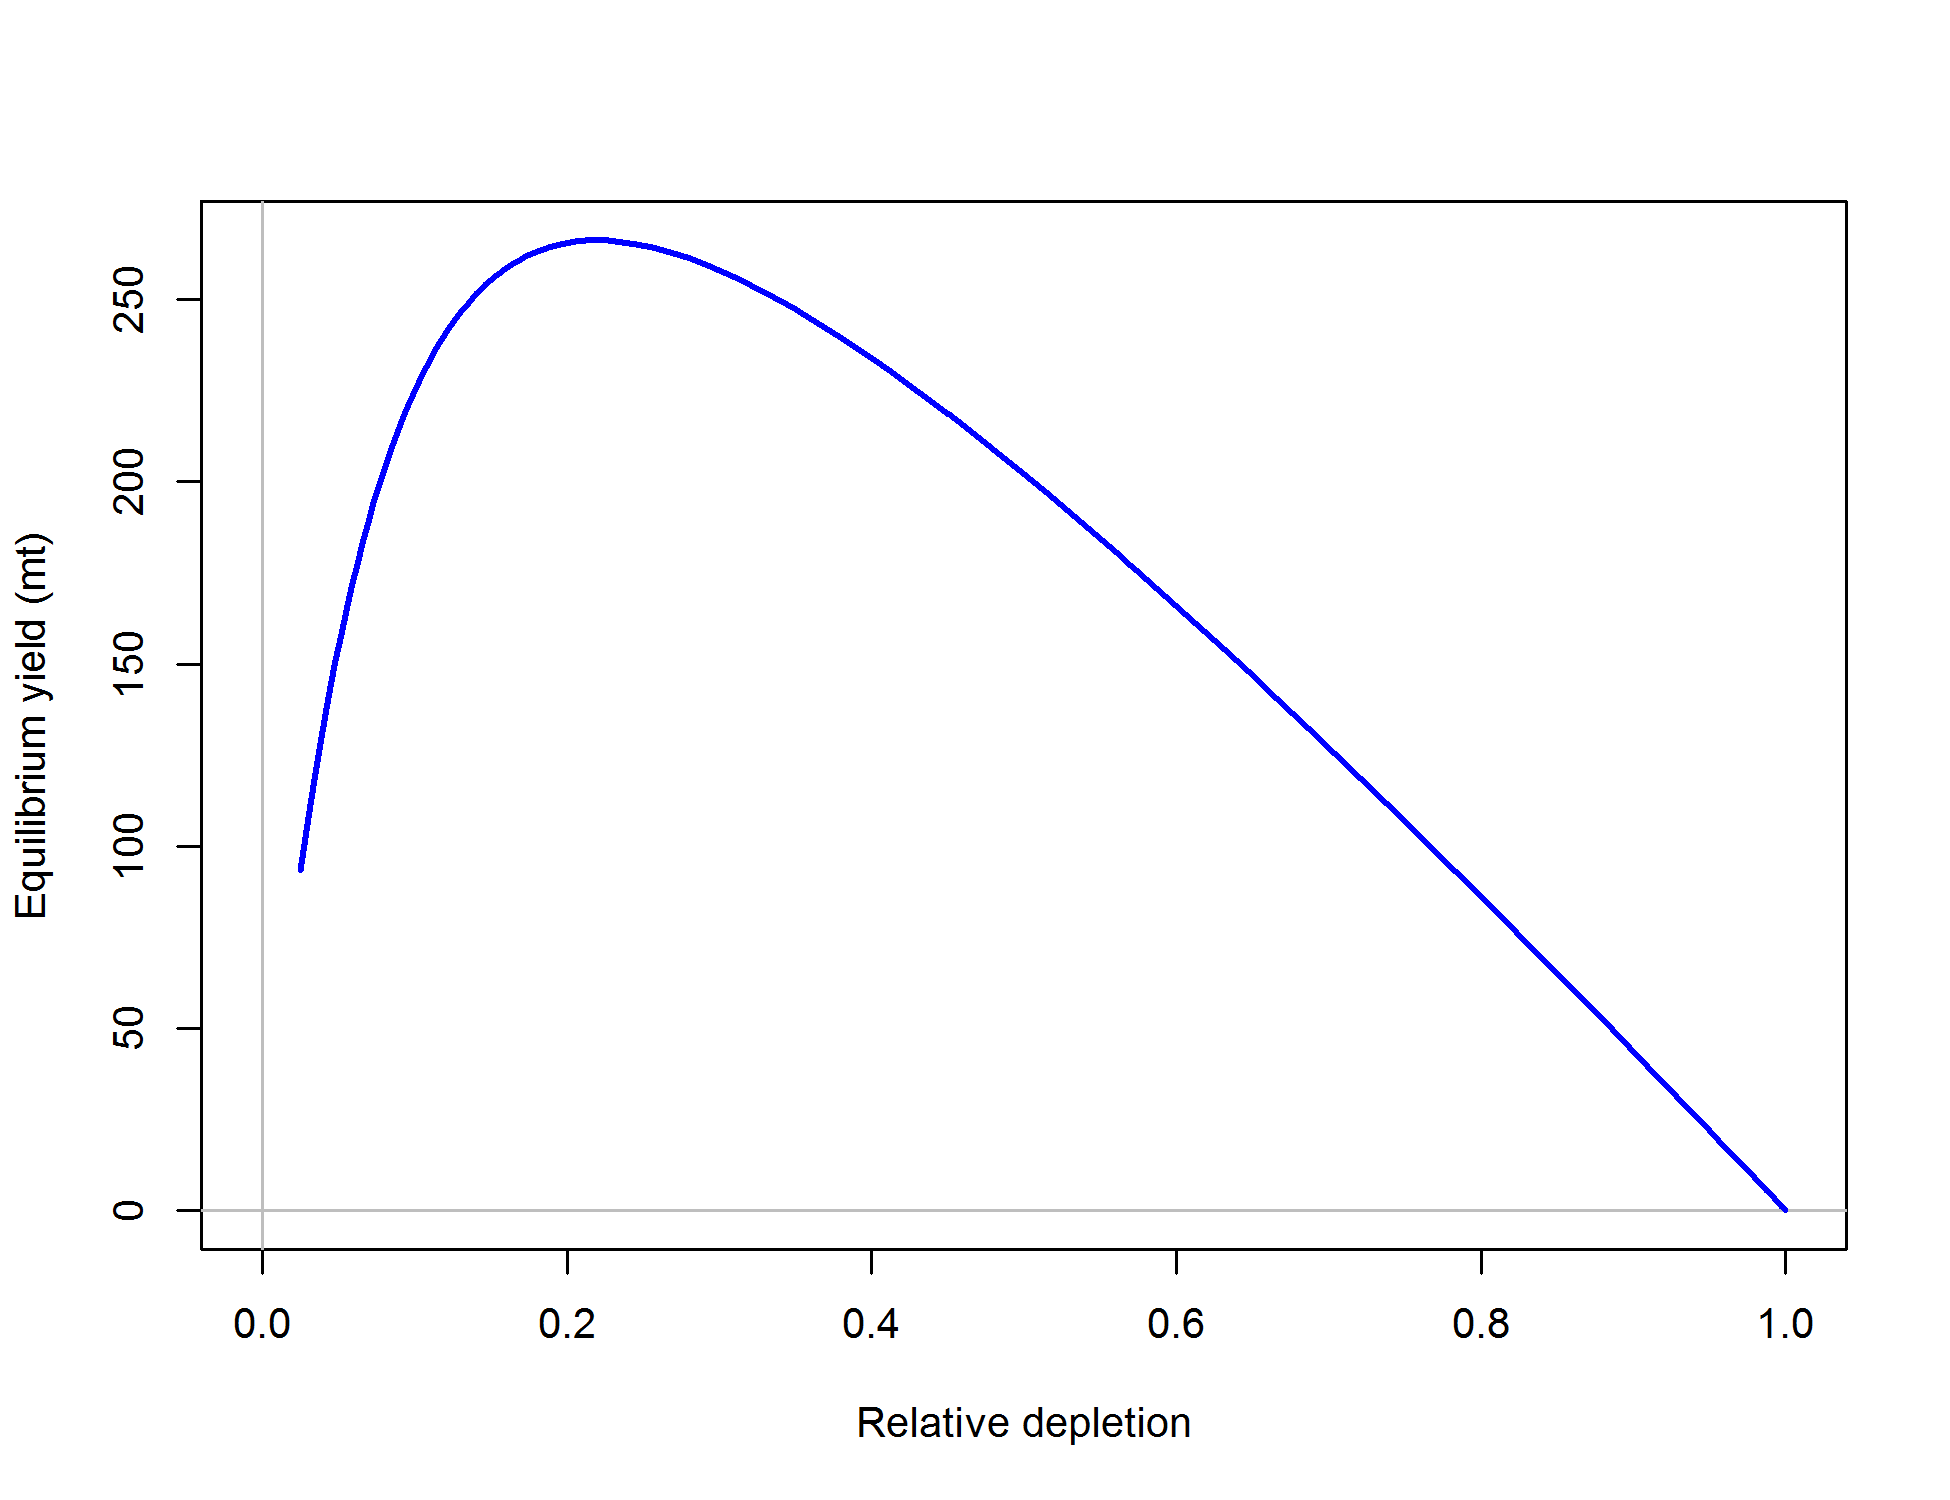
\includegraphics{r4ss/plots_mod1/yield1_yield_curve.png}
\caption{Equilibrium yield curve for the base case model. Values are
based on the 2016 fishery selectivity and with steepness fixed
at\ldots{} \label{fig:Yield_all}}
\end{figure}

\FloatBarrier

\newpage

\subsection*{Research And Data Needs}\label{research-and-data-needs}
\addcontentsline{toc}{subsection}{Research And Data Needs}

We recommend the following research be conducted before the next
assessment:

\begin{enumerate}

\item List item No. 1 in the list

\item List item No. 2 in the list, etc.

\end{enumerate}

\subsection*{Rebuilding Projections}\label{rebuilding-projections}
\addcontentsline{toc}{subsection}{Rebuilding Projections}

\FloatBarrier

\newpage

\renewcommand{\thefigure}{\arabic{figure}}
\renewcommand{\thetable}{\arabic{table}}

\setcounter{figure}{0} \setcounter{table}{0}

\section{Introduction}\label{introduction}

\subsection{Basic Information}\label{basic-information}

California scorpionfish (\emph{Scorpaena guttata}), also known locally
as sculpin or spotted scorpionfish, originates from the Greek word for
scorpionfishes and \emph{guttata} is Latin for speckled. California
scorpionfish is a medium-bodied fish and like other species in the genus
Scorpaena, it produces a toxin in its dorsal, anal, and pectoral fin
spines, which produces intense, painful wounds (Love et al.
\protect\hyperlink{ref-Love1987}{1987}). Scorpionfish are very resistant
to hooking mortality and have shown survival under extreme conditions.

Its range extends from central California (Santa Cruz) to the Gulf of
California, although within U.S. waters they are most common in the
Southern California Bight (Eschmeyer et al.
\protect\hyperlink{ref-Eschmeyer1983}{1983}, Love et al.
\protect\hyperlink{ref-Love1987}{1987}). The species generally inhabits
rocky reefs, caves and crevices, but in certain areas and seasons it
aggregates over sandy or muddy substrate (Love et al.
\protect\hyperlink{ref-Love1987}{1987}, Frey n.d.). California
scorpionfish have been observed from the intertidal to 600 ft with a
preferred depth range from 20-450 ft.

Males and females show different growth rates, with females growing to a
larger size than males, and the sexes exhibit different length-weight
relationships (Love et al. \protect\hyperlink{ref-Love1987}{1987}). Few
California scorpionfish are mature at one year old (14 cm TL).
Fifty-percent of fish mature at 17-18 cm (2 years old) and all by 22 cm
(4 years old) (Love et al. \protect\hyperlink{ref-Love1987}{1987}).

California scorpionfish feed on a wide variety of mobile prey, including
crabs, fishes (e.g., include northern anchovy, spotted cusk-eel),
octopi, isopods and shrimp, (Taylor
\protect\hyperlink{ref-Taylor1963}{1963}, Quast
\protect\hyperlink{ref-Quast1968}{1968}, Love et al.
\protect\hyperlink{ref-Love1987}{1987}, TuRNER et al. n.d.). The species
is nocturnal, but have been observed feeding during the day. Predation
on scorpionfish is believed to be low, but one individual was found in
the gut of a leopard shark (Love pers comm.).

California scorpionfish utilize the ``explosive breeding assemblage''
reproductive mode in which fish migrate to, and aggregate at traditional
spawning sites for brief periods (Love et al.
\protect\hyperlink{ref-Love1987}{1987}). California scorpionfish migrate
to deeper waters (120-360 ft) to spawn during May-August, with peak
spawning occurring July. The species is oviparous, producing floating,
gelatinous egg masses in which the eggs are embedded in a single layer
(Orton \protect\hyperlink{ref-Orton1955}{1955}). and it is believed that
spawning takes place just before, and perhaps after dawn, in the water
column (Love et al. \protect\hyperlink{ref-Love1987}{1987}). Tagging
data suggest California scorpionfish return to the same spawning site,
but information is not available on non-spawning season site fidelity.

Little is known about California scorpionfish larvae. The CalCOFI survey
observed 463 California scorpionfish larvae from 1977-2000, with the
majority at station close to Oxnard (east of the Channel Islands)
(Moser, H. G., R. L. Charter, P. E. Smith, D. A. Ambrose, W. Watson et
al. \protect\hyperlink{ref-Moser2002}{2002}). Higher densities of larvae
have been observed in the CalCOFI stations throughout Baja, peaking
south of Punta Eugenia from July to September. The hatching length is
reported as 1.9-2.0 mm (Washington et al. n.d.) and transformation
length of greater than 1.3 cm (Washington et al. n.d.) less than 2.1 cm
(Moser n.d.).

\subsection{Map}\label{map}

A map showing the scope of the assessment and depicting boundaries for
fisheries or data collection strata is provided in Figure
\ref{fig:boundary_map}.

\subsection{Life History}\label{life-history}

\subsection{Ecosystem Considerations}\label{ecosystem-considerations-1}

In this assessment, ecosystem considerations were not explicitly
included in the analysis. This is primarily due to a lack of relevant
data and results of analyses (conducted elsewhere) that could contribute
ecosystem-related quantitative information for the assessment.

\subsection{Fishery Information}\label{fishery-information}

Rockfish example: The rockfish fishery off the U.S. Pacific coast first
developed off California in the late 19th century as a hook-and-line
fishery (Love et al. \protect\hyperlink{ref-Love2002}{2002}).\\
The rockfish trawl fishery was established in the early 1940s, when the
United States became involved in World War II and wartime shortage of
red meat created an increased demand for other sources of protein (Harry
and Morgan \protect\hyperlink{ref-Harry1961}{1961}, Alverson et al.
\protect\hyperlink{ref-Alverson1964}{1964}). Etc\ldots{}.

\subsection{Summary of Management
History}\label{summary-of-management-history}

Prior to the adoption of the Pacific Coast Groundfish Fishery Management
Plan (FMP) in 1982, California scorpionfish (\emph{Scorpaena guttata})
was managed through a regulatory process that included the California
Department of Fish and Wildlife (CDFW) along with either the California
State Legislature or the Fish and Game Commission (FGC) depending on the
sector (recreation or commercial) and fishery. With implementation of
the Pacific Coast Groundfish FMP, California scorpionfish came under the
management authority of the Pacific Fishery Management Council (PFMC),
being incorporated, along with all genera and species of the family
Scorpaenidae, into a federal rockfish classification and managed as part
of ``Remaining Rockfish'' under the larger heading of ``Other Rockfish''
((Pacific Fishery Management Council (Institution/Organization)
\protect\hyperlink{ref-PFMC2002}{2002},
\protect\hyperlink{ref-PFMC2004}{2004}), Tables 31-39).

The ABCs provided by the PFMC's Groundfish Management Team (GMT) in the
1980's were based on an analysis of commercial landings from the 1960's
and 1970's. For this analysis, most of the rockfishes were lumped into
one large group. This analysis indicated that the landings for rockfish
in the Monterey-Conception area were at or near ABC levels (Pacific
Fishery Management Council (Institution/Organization)
\protect\hyperlink{ref-PFMC1993}{1993}). To keep landings within these
adopted harvest targets, the Pacific Coast Groundfish FMP provided the
Council with a variety of management tools including area closures,
season closures, gear restrictions, and, for the commercial sector,
cumulative limits (generally for two-month periods). With the
implementation of a federal groundfish restricted access program in
1994, allocations of total catch and cumulative limits began to be
specifically set for open access (including most of California's
commercial fisheries that target California scorpionfish in Southern
California) and limited entry fisheries (Pacific Fishery Management
Council (Institution/Organization)
\protect\hyperlink{ref-PFMC2002}{2002},
\protect\hyperlink{ref-PFMC2004}{2004}). As a result, in the later
1990'ss as commercial landings decreased and recreational harvest became
a greater proportion of the available harvest.

Beginning in 1997, California scorpionfish was managed as part of the
Sebastes complex-south, Other Rockfish category. (\emph{Sebastes}
complex-south included the Eureka, Monterey, and Conception areas while
Sebastes complex-north included the Vancouver and Columbia areas.) The
PFMC's rockfish management structure changed significantly in 2000 with
the replacement of the \emph{Sebastes} complex -north and -south areas
with Minor Rockfish North (now covering the Vancouver, Columbia, and
Eureka areas) and Minor Rockfish South (now Monterey and Conception
areas only). The OY for these two groups (which continued to be
calculated as 0.50 of the ABC) was further divided (between north and
south of \(40^\circ 10^\prime\) N. latitude) into nearshore, shelf, and
slope rockfish categories with allocations set for Limited Entry and
Open Access fisheries within each of these three categories (January 4,
2000, 65 FR 221; (Pacific Fishery Management Council
(Institution/Organization) \protect\hyperlink{ref-PFMC2002}{2002}),
Tables 54-55). Because of its depth range and southern distribution,
California scorpionfish was included within the Minor Rockfish South,
Other Rockfish ABC and managed under the south of \(40^\circ 10^\prime\)
N. latitude nearshore rockfish OY and trip limits ((Pacific Fishery
Management Council (Institution/Organization)
\protect\hyperlink{ref-PFMC2002}{2002}), Table 29).

Along with the above changes, in 2000 the southern area divided into two
separate management areas at Point Lopez, \(36^\circ 00^\prime\) N.
latitude. This was followed in 2001 with the implementation of the
northern rockfish and lingcod management area between
(\(40^\circ 10^\prime\) N. latitude) and Point Conception
(\(34^\circ 27^\prime\) N. latitude); and the southern rockfish and
lingcod management area between Point Conception and the U.S.- Mexico
border. These were later revised starting in 2004 with the northern
rockfish and lingcod management area redefined as ocean waters from the
Oregon-California border (\(42^\circ 00^\prime\) N. latitude) to
\(40^\circ 10^\prime\) N. latitude, the central rockfish and lingcod
management area defined as ocean waters from \(40^\circ 10^\prime\) N.
latitude to Point Conception, and the southern rockfish and management
area continuing to be defined as ocean waters from Point Conception to
the U.S.-Mexico border.

Cowcod Conservation Areas (CCAs) also were established in 2001 to reduce
fishing effort for cowcod rockfish ((Pacific Fishery Management Council
(Institution/Organization) \protect\hyperlink{ref-PFMC2002}{2002}),
Table 29). These areas were closed to all recreational and commercial
fishing for groundfish except for minor nearshore rockfish1 (including
California scorpionfish) within waters less than 20 fathoms. In
addition, Rockfish Conservation Areas (RCAs) were established in 2003 to
allow for the closure of specific area and depth ranges along the West
Coast for the purpose of reducing fishing effort for shelf and slope
rockfish. The California Rockfish Conservation Area (CRCA) was defined
as those ocean waters south \(40^\circ 10^\prime\) N. latitude to the
U.S.-Mexico border with different depth zones specified for the areas
north and south of Pt. Reyes (\(37^\circ 59.73^\prime\) N. latitude).

During the late 1990's and early 2000's, major changes also occurred in
the way that California managed its nearshore fishery. The Marine Life
Management Act (MLMA), which was passed in 1998 by the California
Legislature and enacted in 1999, required that the FGC adopt an FMP for
nearshore finfish. It also gave authority to the FGC to regulate
commercial and recreational nearshore fisheries through FMPs and
provided broad authority to adopt regulations for the nearshore fishery
during the time prior to adoption of the nearshore finfish FMP. Within
this legislation, the Legislature also included commercial size limits
for nine nearshore species including California scorpionfish (10-inch
minimum size) and a requirement that commercial fishermen landing these
nine nearshore species possess a nearshore permit.

Following adoption of the Nearshore FMP and accompanying regulations by
the FGC in fall of 2002, the FGC adopted regulations in November 2002
which established a set of marine reserves around the Channel Islands in
Southern California (which became effective April 2003) and adopted a
nearshore restricted access program in December 2002 (which included the
establishment of a Deeper Nearshore Permit) to be effective starting in
the 2003 fishing year.

Although the Nearshore FMP provided for the management of the nearshore
rockfish and California scorpionfish, management authority for these
species continued to reside with the Council. Even so, for the 2003 and
subsequent fishery seasons, the State provided recommendations to the
Council specific to the nearshore species that followed the directives
set out in the Nearshore FMP. These recommendations, which the Council
incorporated into the 2003 management specifications, included a
recalculated OY for Minor Rockfish South - Nearshore, division of the
Minor Rockfish South - Nearshore into three groups (shallow nearshore
rockfish; deeper nearshore rockfish; and California scorpionfish), and
specific harvest targets and recreational and commercial allocations for
each of these groups.

Also, since the enactment of the MLMA, the Council and State in a
coordinated effort developed and adopted various management
specifications to keep harvest within the harvest targets, including
seasonal and area closures (e.g.~the CCAs; a closure of Cordell Banks to
specific fishing), depth restrictions, minimum size limits, and bag
limits to regulate the recreational fishery and license and permit
regulations, finfish trap permits, gear restrictions, seasonal and area
closures (e.g.~the RCAs and CCAs; a closure of Cordell Banks to specific
fishing), depth restrictions, trip limits, and minimum size imits to
regulate the commercial fishery.

\subsection{Management Performance}\label{management-performance-1}

Management performance table: (Table \ref{tab:mnmgt_perform})\\
A summary of these values as well as other base case summary results can
be found in Table \ref{tab:base_summary}.

\subsection{Fisheries off Mexico}\label{fisheries-off-mexico}

Include if necessary.

\section{Assessment}\label{assessment}

\subsection{Data}\label{data}

Data used in the California scorpionfish assessment are summarized in
Figure \ref{fig:data_plot}.\\
A description of each data source is below.

\subsubsection{Commercial Fishery
Landings}\label{commercial-fishery-landings}

\textbf{Sub-heading 1}

\textbf{Sub-heading 2}

\textbf{Sub-heading 3}

\subsubsection{Sport Fishery Removals}\label{sport-fishery-removals}

\textbf{Sub-heading 1}

\textbf{Sub-heading 2}

\textbf{Sub-heading 3}

\subsubsection{Estimated Discards}\label{estimated-discards}

\textbf{Sub-heading 1}

\textbf{Sub-heading 2}

\textbf{Sub-heading 3}

\subsubsection{Abundance Indices}\label{abundance-indices}

\textbf{Sub-heading 1}

\textbf{Sub-heading 2}

\subsubsection{Fishery-Independent Data: possible
sources}\label{fishery-independent-data-possible-sources}

\emph{Northwest Fisheries Science Center (NWFSC) slope survey}\\
The NWFSC slope survey was conducted annually from 1999 to 2002.\\
The depth range of this survey is 100-700 fm.

\emph{Northwest Fisheries Science Center (NWFSC) shelf-slope survey}\\
This survey is referred to as the ``combo,'' conducted annually since
2003.\\
The survey consistently covered depths between 30 and 700 fm.

\emph{Alaska Fisheries Science Center (AFSC) shelf survey}\\
The survey, often referred to as the ``triennial'' survey was conducted
every third year between 1977 and (and conducted in 2004 by the NWFSC
using the same protocols). The triennial survey trawls in depths of 30
to 275 fm.

\emph{Partnership For Interdisciplinary Studies of Coastal Oceans
(PISCO)}\\
Blurb on species presence in PISCO surveys

\subsubsection{Biological Parameters and
Data}\label{biological-parameters-and-data}

\textbf{Length And Age Compositions}

Include: Sample size information for length and age composition data by
area, year, gear, market category, etc., including both the number of
trips and fish sampled.

Length compositions were provided from the following sources, with brief
descriptions below:

\begin{itemize}[noitemsep,nolistsep,topsep=0pt]
  \item CDFW market category study (\emph{commercial dead fish},1996-2003)    
  \item CALCOM (\emph{commercial dead fish}, 2013-2016)    
  \item CDFW onboard observer (\emph{recreational charter discards}, 2003-2016)    
  \item Ally onboard observer study (\emph{recreational charter discards}, 1984-1989)  
  \item California recreational sources combined (\emph{recreational charter retained catch})     
    \begin{itemize}[noitemsep,nolistsep]
      \item CDFW and Ally onboard observer surveys (1984-1989)     
      \item Collins and Crooke onboard observer surveys (1975-1978)     
      \item MRFSS (1980-2003)     
      \item CRFS (2004-2014)
    \end{itemize}
 \item California recreational sources combined (\emph{private mode retained catch})      
    \begin{itemize}[noitemsep,nolistsep]   
      \item MRFSS (1980-2003)      
      \item CRFS (2004-2016)  
    \end{itemize}
 \item Sanitation district trawl surveys (\emph{research}, 1970-2016)      
 \item CSUN/VRG gillnet survey (\emph{research}, 1995-2008)        
 \item Power plant impingement surveys (\emph{research}, 1974-2016) 
 \item Southern California Bight trawl survey (\emph{research}, 1994,1998,2003,2008,2013) 
\end{itemize}

\emph{Recreational: California MRFSS And CRFS Length Composition Data}
Individual fish lengths recorded by MRFSS (1980-2003) and CRFS
(2004-2011) samplers were downloaded from the RecFIN website
(www.recfin.org). CRFS data from 2012-2014 were obtained directly from
CDFW.

\emph{Commercial: PacFIN}

\emph{Research: NWFSC shelf-slope survey}

\emph{Research: NWFSC slope survey}

\vspace{.5cm}

\textbf{Age Structures} Age data were provided from the NWFSC trawl
survey from 2005-2016.

Length-at-age was initially estimated external to the population
dynamics models using the von Bertalanffy growth curve (Bertalanffy
\protect\hyperlink{ref-vonB1938}{1938}),
\(L_i = L_{\infty}e^{(-k[t-t_0])}\), where \(L_i\) is the length (cm) at
age \(i\), \(t\) is age in years, \(k\) is rate of increase in growth,
\(t_0\) is the intercept, and \(L_{\infty}\) is the asymptotic length.

\vspace{.5cm}

\textbf{Aging Precision And Bias}

\vspace{.5cm}

\textbf{Weight-Length}

The weight-length relationship is based on the standard power function:
\(W = \alpha(L^\beta)\) where \(W\) is individual weight (kg), \(L\) is
length (cm), and \(\alpha\) and \(\beta\) are coefficients used as
constants.

\vspace{.5cm}

\textbf{Maturity And Fecundity}

\vspace{.5cm}

\textbf{Natural Mortality} Hamel
(\protect\hyperlink{ref-Hamel2015}{2015}) developed a method for
combining meta-analytic approaches to relating the natural mortality
rate \(M\) to other life-history parameters such as longevity, size,
growth rate and reproductive effort, to provide a prior on M. In that
same issue of ICESJMS, Then et al.
(\protect\hyperlink{ref-Then2015}{2015}), provided an updated data set
of estimates of \(M\) and related life history parameters across a large
number of fish species, from which to develop an \(M\) estimator for
fish species in general. They concluded by recommending \(M\) estimates
be based on maximum age alone, based on an updated Hoenig non-linear
least squares (nls) estimator \(M= 4.899*{A_{max}}^{-.916}\). The
approach of basing \(M\) priors on maximum age alone was one that was
already being used for west coast rockfish assessments. However, in
fitting the alternative model forms relating \(-.916M\) to \(A_{max}\),
Then et al. (\protect\hyperlink{ref-Then2015}{2015}) did not
consistently apply their transformation. In particular, in real space,
one would expect substantial heteroscedasticity in both the observation
and process error associated with the observed relationship of \(M\) to
\(A_{max}\). Therefore, it would be reasonable to fit all models under a
log transformation. This was not done. Revaluating the data used in Then
et al. (\protect\hyperlink{ref-Then2015}{2015}) by fitting the
one-parameter \(A_{max}\) model under a log-log transformation (such
that the slope is forced to be -1 in the transformed space (as in Hamel
(\protect\hyperlink{ref-Hamel2015}{2015})), the point estimate for \(M\)
is:

\begin{equation}
M = \frac{5.4}{A_{max}}
\end{equation}

The above is also the median of the prior. The prior is defined as a
lognormal with mean \(ln\frac{5.4}{A_{max}}\) and SE = 0.4384343. Using
a maximum age of 21 the point estimate and median of the prior is
0.2545, which is used as a prior for females in the assessment model.

\vspace{.5cm}

\textbf{Sex ratios}

\subsubsection{Environmental Or Ecosystem Data Included In The
Assessment}\label{environmental-or-ecosystem-data-included-in-the-assessment}

\subsection{History Of Modeling Approaches Used For This
Stock}\label{history-of-modeling-approaches-used-for-this-stock}

\subsubsection{Previous Assessments}\label{previous-assessments}

\subsubsection{2005 Assessment
Recommendations}\label{assessment-recommendations}

Include: Response to STAR panel recommendations from the most recent
previous assessment.

\begin{description}[style=unboxed]

  \item[Recommendation 1: The sanitation surveys conducted to track the impact 
  of sewage outfall provided a fishery independent index of abundance for 
  scorpionfish. This data source should be more fully explored for other 
  near-shore species of recreational or commercial interest. Methods should 
  be developed to produce a more statistically rigorous index from the 
  separate surveys.] \hfill \\

   STAT response: Data from all sanitation districts in southern California 
   were obtained for this assessment.  All of the data were pooled across
   surveys to develop one index of abundance using the delta-GLM method

\item[Recommendation 2: An age, growth and maturity study for scorpionfish is 
needed.  Although there has been previous research on scorpionfish age and growth, 
the available information is not appropriate for stock assessment modeling.] \hfill \\

  STAT response: Age data are available from the NWFSC trawl survey from 2005-2016.
  THere have been no additional studies on growth or maturity for California 
  scorpionfish since the 2005 assessment.

\item[Recommendation 3: Location information for the historic groundfish data 
of all species is currently available, in hard copy form only, from the 
California Department of Fish and Game. Putting this information into electronic 
format would greatly improve the ability to assign catches of all species to 
specific stocks on a trip-by-trip basis.] \hfill \\

  STAT response: The location-sepciic catches referred to above have been
  key-punched and are available in electornic form from the SWFSC, Santa Cruz.

\item[Recommendation 4: The SS2 model should be modified to allow for projections 
of user-specified recruitment at user defined values. It would be most helpful if 
the default harvest policies were then recalculated automatically for these 
user-specified recruitments.] \hfill \\

  STAT response: The status of this within Stock Synthesis is unknown.
  
\end{description}

\subsection{Model Description}\label{model-description}

\subsubsection{Transition To The Current Stock
Assessment}\label{transition-to-the-current-stock-assessment}

Include: Complete description of any new modeling approaches

Below, we describe the most important changes made since the last full
assessment and explain rationale for each change.:

\begin{enumerate}
\def\labelenumi{\arabic{enumi}.}
\item
  Change No. 1. \emph{Rationale}: blah blah blah.
\item
  Change No. 2. \emph{Rationale}: blah blah blah.
\item
  Change No. 3. \emph{Rationale}: Continue list as needed.
\end{enumerate}

\subsubsection{Definition of Fleets and
Areas}\label{definition-of-fleets-and-areas}

We generated data sources for each of the models. Fleets by model
include:

\textbf{Model Region 1 or remove this line if only one model}

\emph{Commercial}: The commercial fleets include\ldots{}

\emph{Recreational}: The recreational fleets include\ldots{}

\emph{Research}: Research derived-data include\ldots{}

\subsubsection{Summary of Data for Fleets and
Areas}\label{summary-of-data-for-fleets-and-areas}

\subsubsection{Modeling Software}\label{modeling-software}

The STAT team used Stock Synthesis 3 version 3.30.0.4 by Dr.~Richard
Methot at the NWFSC. This most recent version was used, since it
included improvements and corrections to older versions. The r4SS
package (GitHub release number v1.27.0) was used to post-processing
output data from Stock Synthesis.

\subsubsection{Data Weighting}\label{data-weighting}

Citation for Francis method (Francis
\protect\hyperlink{ref-Francis2011}{2011})\\
Citation for Ianelli-McAllister harmonic mean method (McAllister and
Ianelli \protect\hyperlink{ref-McAllister1997}{1997})

\subsubsection{Priors}\label{priors}

Citation for Hamel prior on natural mortality (Hamel
\protect\hyperlink{ref-Hamel2015}{2015})

\subsubsection{General Model
Specifications}\label{general-model-specifications}

Model data, control, starter, and forecast files can be found in
Appendices A-D.

\subsubsection{Estimated And Fixed
Parameters}\label{estimated-and-fixed-parameters}

A full list of all estimated and fixed parameters is provided in
Tables\ldots{}. Estimated and fixed parameters tables currently read in
from .csv file, EXAMPLE: Table \ref{tab:Model1_params}

\subsection{Model Selection and
Evaluation}\label{model-selection-and-evaluation}

\subsubsection{Key Assumptions and Structural
Choices}\label{key-assumptions-and-structural-choices}

Include: Evidence of search for balance between model realism and
parsimony.\\
Comparison of key model assumptions, include comparisons based on nested
models (e.g., asymptotic vs.~domed selectivities, constant
vs.~time-varying selectivities).

\subsubsection{Alternate Models
Considered}\label{alternate-models-considered}

Include: Summary of alternate model configurations that were tried but
rejected.

\subsubsection{Convergence}\label{convergence}

Include: Randomization run results or other evidence of search for
global best estimates.

Convergence testing through use of dispersed starting values often
requires extreme values to actually explore new areas of the
multivariate likelihood surface. Jitter is a SS option that generates
random starting values from a normal distribution logistically
transformed into each parameter's range (Methot
\protect\hyperlink{ref-Methot2015}{2015}). Table \ref{tab:jitter} shows
the results of running 100 jitters for each pre-STAR base model\ldots{}.

\subsection{Response To The Current STAR Panel
Requests}\label{response-to-the-current-star-panel-requests}

\begin{description}[style=unboxed]

\item[Request No. 1: Add after STAR panel.] \hfill \\

    \textbf{Rationale:} Add after STAR panel.  

    \textbf{STAT Response:} Add after STAR panel.

\item[Request No. 2: Add after STAR panel.] \hfill \\

    \textbf{Rationale:} Add after STAR panel.

    \textbf{STAT Response:} Add after STAR panel.

\item[Request No. 3: Add after STAR panel.] \hfill \\

    \textbf{Rationale:} Add after STAR panel.
  
    \textbf{STAT Response:} Add after STAR panel.

\item[Request No. 4: Example of a request that may have a list:] \hfill \\
\begin{itemize}
\item \textbf{Item No. 1}
\item \textbf{Item No. 2}
\item \textbf{Item No. 3, etc.}
\end{itemize}

    \textbf{Rationale:} Add after STAR panel.

    \textbf{STAT Response:} Continue requests as needed.


\end{description}

\subsection{Model 1}\label{model-1}

\subsubsection{Model 1 Base Case
Results}\label{model-1-base-case-results}

Table \ref{tab:Model1_params}

\subsubsection{Model 1 Uncertainty and Sensitivity
Analyses}\label{model-1-uncertainty-and-sensitivity-analyses}

Table \ref{tab:Sensitivity_model1}

\subsubsection{Model 1 Retrospective
Analysis}\label{model-1-retrospective-analysis}

\subsubsection{Model 1 Likelihood
Profiles}\label{model-1-likelihood-profiles}

\subsubsection{Model 1 Harvest Control Rules (CPS
only)}\label{model-1-harvest-control-rules-cps-only}

\subsubsection{Model 1 Reference Points (groundfish
only)}\label{model-1-reference-points-groundfish-only}

Intro sentence or two\ldots{}.(Table \ref{tab:Timeseries_mod1}).

Equilibrium yield at the proxy \(F_{MSY}\) harvest rate corresponding to
\(SPR_{50\%}\) is 276.8 mt. Table \ref{tab:Ref_pts_mod1} shows the full
suite of estimated reference points for the northern area model and
Figure \ref{fig:Yield_all} shows the equilibrium yield curve.

\section{Harvest Projections and Decision
Tables}\label{harvest-projections-and-decision-tables}

Table \ref{tab:mnmgt_perform}

\textbf{Model 1 Projections and Decision Table (groundfish only)} (Table
\ref{tab:Forecast_mod1}

Table \ref{tab:Decision_table_mod1}

\textbf{Model 2 Projections and Decision Table (groundfish only)}

\textbf{Model 3 Projections and Decision Table (groundfish only)}

\section{Regional Management
Considerations}\label{regional-management-considerations}

\begin{enumerate}
\def\labelenumi{\arabic{enumi}.}
\tightlist
\item
  For stocks where current practice is to allocate harvests by
  management area, a recommended method of allocating harvests based on
  the distribution of biomass should be provided. The MT advisor should
  be consulted on the appropriate management areas for each stock.
\item
  Discuss whether a regional management approach makes sense for the
  species from a biological perspective.
\item
  If there are insufficient data to analyze a regional management
  approach, what are the research and data needs to answer this
  question?
\end{enumerate}

\section{Research Needs}\label{research-needs}

\begin{enumerate}

\item Research need No. 1

\item Research need No. 2

\item Research need No. 3

\item etc.

\end{enumerate}

\section{Acknowledgments}\label{acknowledgments}

Include: STAR panel members and affiliations as well as names and
affiliations of persons who contributed data, advice or information but
were not part of the assessment team. Not required in draft assessment
undergoing review.

\newpage

\FloatBarrier

\section{Tables}\label{tables}

\begin{longtable}{c>{\centering}p{1in}>{\centering}p{.6in}>{\centering}p{.6in}>{\centering}p{.6in}>{\centering}p{1in}l}
\caption{Commercial removals (mt) from the commercial 
                                fisheries, north and source of Florence, OR.} \\ 
  \hline
Year & Hook-and-line & Trawl & Gillnet & Mexico & Total U.S. Removals & Source \\ 
  \hline \endhead  \hline
1916 & 3.64 & 0.00 & 0.00 & 0.00 & 3.64 & CDFG Bulletins \\ 
  1917 & 7.90 & 0.00 & 0.00 & 0.00 & 7.90 & CDFG Bulletins \\ 
  1918 & 12.81 & 0.00 & 0.00 & 0.00 & 12.81 & CDFG Bulletins \\ 
  1919 & 11.54 & 0.00 & 0.00 & 0.00 & 11.54 & CDFG Bulletins \\ 
  1920 & 16.18 & 0.00 & 0.00 & 0.00 & 16.18 & CDFG Bulletins \\ 
  1921 & 26.48 & 0.00 & 0.00 & 0.00 & 26.48 & CDFG Bulletins \\ 
  1922 & 19.11 & 0.00 & 0.00 & 0.00 & 19.11 & CDFG Bulletins \\ 
  1923 & 27.43 & 0.00 & 0.00 & 0.00 & 27.43 & CDFG Bulletins \\ 
  1924 & 49.47 & 0.00 & 0.00 & 0.00 & 49.47 & CDFG Bulletins \\ 
  1925 & 101.20 & 0.00 & 0.00 & 0.00 & 101.20 & CDFG Bulletins \\ 
  1926 & 49.02 & 0.00 & 0.00 & 0.00 & 49.02 & CDFG Bulletins \\ 
  1927 & 51.46 & 0.00 & 0.00 & 0.00 & 51.46 & CDFG Bulletins \\ 
  1928 & 44.04 & 0.00 & 0.00 & 0.00 & 44.04 & CDFG Bulletins \\ 
  1929 & 48.90 & 0.00 & 0.00 & 0.00 & 48.90 & CDFG Bulletins \\ 
  1930 & 40.19 & 0.00 & 0.00 & 0.00 & 40.19 & CDFG Bulletins \\ 
  1931 & 41.54 & 0.00 & 0.00 & 0.05 & 41.54 & CDFG Bulletins \\ 
  1932 & 38.78 & 0.00 & 0.00 & 0.00 & 38.78 & CDFG Bulletins \\ 
  1933 & 29.10 & 0.00 & 0.00 & 0.00 & 29.10 & CDFG Bulletins \\ 
  1934 & 29.91 & 0.00 & 0.00 & 0.00 & 29.91 & CDFG Bulletins \\ 
  1935 & 30.76 & 0.00 & 0.00 & 0.79 & 30.76 & CDFG Bulletins \\ 
  1936 & 49.75 & 0.00 & 0.00 & 0.34 & 49.75 & CDFG Bulletins \\ 
  1937 & 62.19 & 0.00 & 0.00 & 0.09 & 62.19 & CDFG Bulletins \\ 
  1938 & 70.44 & 0.00 & 0.00 & 0.05 & 70.44 & CDFG Bulletins \\ 
  1939 & 58.29 & 0.00 & 0.00 & 0.06 & 58.29 & CDFG Bulletins \\ 
  1940 & 55.37 & 0.00 & 0.00 & 0.03 & 55.37 & CDFG Bulletins \\ 
  1941 & 43.07 & 0.00 & 0.00 & 0.14 & 43.07 & CDFG Bulletins \\ 
  1942 & 20.00 & 0.00 & 0.00 & 0.11 & 20.00 & CDFG Bulletins \\ 
  1943 & 16.32 & 0.00 & 0.00 & 2.98 & 16.32 & CDFG Bulletins \\ 
  1944 & 24.03 & 0.00 & 0.00 & 1.95 & 24.03 & CDFG Bulletins \\ 
  1945 & 42.13 & 0.00 & 0.00 & 0.81 & 42.13 & CDFG Bulletins \\ 
  1946 & 65.63 & 0.00 & 0.00 & 0.16 & 65.63 & CDFG Bulletins \\ 
  1947 & 56.79 & 0.00 & 0.00 & 0.84 & 56.79 & CDFG Bulletins \\ 
  1948 & 70.17 & 0.00 & 0.00 & 0.18 & 70.17 & CDFG Bulletins \\ 
  1949 & 66.72 & 0.00 & 0.00 & 0.58 & 66.72 & CDFG Bulletins \\ 
  1950 & 63.16 & 0.00 & 0.00 & 0.12 & 63.16 & CDFG Bulletins \\ 
  1951 & 45.85 & 0.00 & 0.00 & 0.16 & 45.85 & CDFG Bulletins \\ 
  1952 & 37.93 & 0.00 & 0.00 & 0.00 & 37.93 & CDFG Bulletins \\ 
  1953 & 54.17 & 0.00 & 0.00 & 0.05 & 54.17 & CDFG Bulletins \\ 
  1954 & 60.92 & 0.00 & 0.00 & 0.00 & 60.92 & CDFG Bulletins \\ 
  1955 & 47.71 & 0.00 & 0.00 & 1.29 & 47.71 & CDFG Bulletins \\ 
  1956 & 45.47 & 0.00 & 0.00 & 0.00 & 45.47 & CDFG Bulletins \\ 
  1957 & 33.23 & 0.00 & 0.00 & 0.00 & 33.23 & CDFG Bulletins \\ 
  1958 & 29.43 & 0.00 & 0.00 & 0.00 & 29.43 & CDFG Bulletins \\ 
  1959 & 16.94 & 0.00 & 0.00 & 0.00 & 16.94 & CDFG Bulletins \\ 
  1960 & 13.25 & 0.00 & 0.00 & 0.00 & 13.25 & CDFG Bulletins \\ 
  1961 & 12.12 & 0.00 & 0.00 & 0.00 & 12.12 & CDFG Bulletins \\ 
  1962 & 26.18 & 0.00 & 0.00 & 0.11 & 26.18 & CDFG Bulletins \\ 
  1963 & 34.11 & 0.00 & 0.00 & 0.14 & 34.11 & CDFG Bulletins \\ 
  1964 & 35.19 & 0.00 & 0.00 & 7.55 & 35.19 & CDFG Bulletins \\ 
  1965 & 34.78 & 0.00 & 0.00 & 2.75 & 34.78 & CDFG Bulletins \\ 
  1966 & 38.31 & 0.00 & 0.00 & 10.90 & 38.31 & CDFG Bulletins \\ 
  1967 & 25.42 & 0.00 & 0.00 & 12.07 & 25.42 & CDFG Bulletins \\ 
  1968 & 40.60 & 0.00 & 0.00 & 16.18 & 40.60 & CDFG Bulletins \\ 
  1969 & 33.28 & 0.28 & 0.10 & 18.72 & 33.66 & CFIS \\ 
  1970 & 34.45 & 0.00 & 0.16 & 35.67 & 34.62 & CFIS \\ 
  1971 & 17.76 & 0.00 & 0.63 & 40.41 & 18.38 & CFIS \\ 
  1972 & 27.84 & 0.11 & 0.13 & 31.81 & 28.08 & CFIS \\ 
  1973 & 16.80 & 0.17 & 0.24 & 54.85 & 17.21 & CFIS \\ 
  1974 & 37.94 & 0.00 & 0.06 & 33.59 & 38.00 & CFIS \\ 
  1975 & 41.95 & 0.02 & 3.03 & 33.64 & 45.01 & CFIS \\ 
  1976 & 15.41 & 0.06 & 0.01 & 63.29 & 15.49 & CFIS \\ 
  1977 & 5.75 & 0.00 & 0.13 & 47.07 & 5.88 & CFIS \\ 
  1978 & 8.99 & 0.00 & 1.26 & 21.62 & 10.25 & CFIS \\ 
  1979 & 8.40 & 0.00 & 0.97 & 5.43 & 9.37 & CFIS \\ 
  1980 & 14.47 & 0.00 & 0.56 & 11.72 & 15.03 & CFIS \\ 
  1981 & 15.48 & 0.01 & 5.93 & 4.09 & 21.41 & CFIS \\ 
  1982 & 17.95 & 0.00 & 1.34 & 8.46 & 19.29 & CFIS \\ 
  1983 & 10.91 & 0.00 & 0.83 & 2.31 & 11.74 & CFIS \\ 
  1984 & 9.89 & 0.15 & 1.07 & 0.08 & 11.11 & CFIS \\ 
  1985 & 12.73 & 0.02 & 2.48 & 0.00 & 15.24 & CFIS \\ 
  1986 & 4.76 & 0.02 & 1.76 & 0.11 & 6.54 & CFIS \\ 
  1987 & 7.46 & 0.11 & 3.99 & 0.00 & 11.56 & CFIS \\ 
  1988 & 7.77 & 0.00 & 3.65 & 0.00 & 11.42 & CFIS \\ 
  1989 & 15.87 & 0.02 & 2.80 & 0.00 & 18.69 & CFIS \\ 
  1990 & 32.07 & 0.78 & 6.17 & 0.00 & 39.01 & CFIS \\ 
  1991 & 20.12 & 4.80 & 3.29 & 0.00 & 28.20 & CFIS \\ 
  1992 & 27.71 & 3.94 & 3.33 & 0.00 & 34.98 & CFIS \\ 
  1993 & 13.72 & 7.76 & 4.66 & 0.22 & 26.14 & CFIS \\ 
  1994 & 34.85 & 13.08 & 1.92 & 0.00 & 49.86 & CFIS \\ 
  1995 & 23.69 & 16.20 & 0.98 & 0.13 & 40.87 & CFIS \\ 
  1996 & 20.17 & 12.97 & 1.19 & 0.00 & 34.33 & CFIS \\ 
  1997 & 20.22 & 13.28 & 3.82 & 0.00 & 37.31 & CFIS \\ 
  1998 & 32.34 & 16.80 & 1.59 & 0.00 & 50.72 & CFIS \\ 
  1999 & 30.88 & 6.56 & 1.78 & 0.00 & 39.22 & CFIS \\ 
  2000 & 11.74 & 4.57 & 2.00 & 0.00 & 18.30 & CFIS \\ 
  2001 & 14.18 & 2.98 & 2.64 & 0.00 & 19.80 & CFIS \\ 
  2002 & 10.09 & 2.16 & 1.18 & 0.00 & 13.43 & CFIS \\ 
  2003 & 2.13 & 2.75 & 0.35 & 0.00 & 5.24 & CFIS \\ 
  2004 & 2.00 & 2.36 & 0.62 & 0.00 & 4.98 & CFIS \\ 
  2005 & 1.47 & 3.12 & 0.70 & 0.00 & 5.29 & CFIS \\ 
  2006 & 0.86 & 1.38 & 0.44 & 0.00 & 2.68 & CFIS \\ 
  2007 & 1.90 & 1.48 & 0.21 & 0.00 & 3.59 & CFIS \\ 
  2008 & 2.46 & 0.86 & 0.28 & 0.00 & 3.61 & CFIS \\ 
  2009 & 2.97 & 0.27 & 0.13 & 0.00 & 3.38 & CFIS \\ 
  2010 & 2.99 & 0.18 & 0.14 & 0.00 & 3.32 & CFIS \\ 
  2011 & 3.24 & 1.05 & 0.24 & 0.00 & 4.54 & CFIS \\ 
  2012 & 3.22 & 0.43 & 0.18 & 0.00 & 3.82 & CFIS \\ 
  2013 & 1.73 & 0.83 & 0.14 & 0.00 & 2.70 & CFIS \\ 
  2014 & 1.03 & 0.13 & 0.04 & 0.00 & 1.19 & CFIS \\ 
  2015 & 2.21 & 0.13 & 0.03 & 0.00 & 2.37 & CFIS \\ 
  2016 & 2.32 & 0.13 & 0.00 & 0.00 & 2.45 & CFIS \\ 
   \hline
\hline
\label{tab:Comm_catches}
\end{longtable}

\begin{longtable}{ccccc}
\caption{Recreational removals (mt) from the party/charter 
                                        (PC) and private (PR) vessels. CDFW provided all 
                                        data. Note: A discard mortality rate of 7% was applied 
                                          to the dead discard removals.} \\ 
  \hline
Year & Private & Party/charter & Dead Discard (all modes) & Total Removals \\ 
  \hline \endhead  \hline
1929 & 0.06 & 0.54 & 0.00 & 0.61 \\ 
  1930 & 0.12 & 1.08 & 0.01 & 1.21 \\ 
  1931 & 0.18 & 1.62 & 0.01 & 1.81 \\ 
  1932 & 0.24 & 2.16 & 0.01 & 2.42 \\ 
  1933 & 0.30 & 2.70 & 0.02 & 3.02 \\ 
  1934 & 0.36 & 3.24 & 0.02 & 3.63 \\ 
  1935 & 0.42 & 3.78 & 0.03 & 4.23 \\ 
  1936 & 0.48 & 4.33 & 0.03 & 4.84 \\ 
  1937 & 0.34 & 3.01 & 0.02 & 3.37 \\ 
  1938 & 0.56 & 5.06 & 0.04 & 5.66 \\ 
  1939 & 0.44 & 3.90 & 0.03 & 4.36 \\ 
  1940 & 0.40 & 3.61 & 0.02 & 4.04 \\ 
  1941 & 0.00 & 0.00 & 0.00 & 0.00 \\ 
  1942 & 0.00 & 0.00 & 0.00 & 0.00 \\ 
  1943 & 0.00 & 0.00 & 0.00 & 0.00 \\ 
  1944 & 0.00 & 0.00 & 0.00 & 0.00 \\ 
  1945 & 0.00 & 0.00 & 0.00 & 0.00 \\ 
  1946 & 0.00 & 0.00 & 0.00 & 0.00 \\ 
  1947 & 1.76 & 15.73 & 0.11 & 17.60 \\ 
  1948 & 3.65 & 32.67 & 0.23 & 36.55 \\ 
  1949 & 2.58 & 23.12 & 0.16 & 25.86 \\ 
  1950 & 3.38 & 30.29 & 0.21 & 33.89 \\ 
  1951 & 2.11 & 18.84 & 0.13 & 21.08 \\ 
  1952 & 2.29 & 20.48 & 0.14 & 22.91 \\ 
  1953 & 1.93 & 17.24 & 0.12 & 19.28 \\ 
  1954 & 2.26 & 20.27 & 0.14 & 22.67 \\ 
  1955 & 1.93 & 17.33 & 0.12 & 19.38 \\ 
  1956 & 1.70 & 15.26 & 0.11 & 17.07 \\ 
  1957 & 0.94 & 8.44 & 0.06 & 9.44 \\ 
  1958 & 0.96 & 8.60 & 0.06 & 9.62 \\ 
  1959 & 0.80 & 7.19 & 0.05 & 8.04 \\ 
  1960 & 1.06 & 9.47 & 0.07 & 10.59 \\ 
  1961 & 1.86 & 16.71 & 0.12 & 18.69 \\ 
  1962 & 2.33 & 20.87 & 0.14 & 23.34 \\ 
  1963 & 3.77 & 33.75 & 0.23 & 37.75 \\ 
  1964 & 5.16 & 46.25 & 0.32 & 51.73 \\ 
  1965 & 5.02 & 45.03 & 0.31 & 50.36 \\ 
  1966 & 6.44 & 43.74 & 0.31 & 50.48 \\ 
  1967 & 7.34 & 39.64 & 0.29 & 47.27 \\ 
  1968 & 8.46 & 37.50 & 0.29 & 46.25 \\ 
  1969 & 10.62 & 39.47 & 0.32 & 50.41 \\ 
  1970 & 16.32 & 51.69 & 0.43 & 68.44 \\ 
  1971 & 19.46 & 53.19 & 0.46 & 73.10 \\ 
  1972 & 15.80 & 37.62 & 0.34 & 53.76 \\ 
  1973 & 25.01 & 52.28 & 0.49 & 77.78 \\ 
  1974 & 29.18 & 53.84 & 0.52 & 83.55 \\ 
  1975 & 31.19 & 51.01 & 0.52 & 82.72 \\ 
  1976 & 20.44 & 29.75 & 0.32 & 50.50 \\ 
  1977 & 35.19 & 45.69 & 0.51 & 81.39 \\ 
  1978 & 23.82 & 27.63 & 0.33 & 51.77 \\ 
  1979 & 49.76 & 40.23 & 0.58 & 90.57 \\ 
  1980 & 53.27 & 52.35 & 3.72 & 109.35 \\ 
  1981 & 41.08 & 44.42 & 2.85 & 88.36 \\ 
  1982 & 49.04 & 40.92 & 2.81 & 92.77 \\ 
  1983 & 12.65 & 35.56 & 0.93 & 49.14 \\ 
  1984 & 27.06 & 31.25 & 0.96 & 59.27 \\ 
  1985 & 28.77 & 39.93 & 1.71 & 70.41 \\ 
  1986 & 24.07 & 42.53 & 3.19 & 69.79 \\ 
  1987 & 23.05 & 31.78 & 3.02 & 57.85 \\ 
  1988 & 106.56 & 76.88 & 5.89 & 189.34 \\ 
  1989 & 56.79 & 79.32 & 7.90 & 144.00 \\ 
  1990 & 95.63 & 92.27 & 1.16 & 189.06 \\ 
  1991 & 107.40 & 103.63 & 1.30 & 212.34 \\ 
  1992 & 31.91 & 44.10 & 3.60 & 79.60 \\ 
  1993 & 23.31 & 43.49 & 2.26 & 69.07 \\ 
  1994 & 45.62 & 54.40 & 6.42 & 106.45 \\ 
  1995 & 28.44 & 57.03 & 6.21 & 91.68 \\ 
  1996 & 30.46 & 67.48 & 4.00 & 101.93 \\ 
  1997 & 24.39 & 77.23 & 2.62 & 104.24 \\ 
  1998 & 32.12 & 75.91 & 2.08 & 110.11 \\ 
  1999 & 50.11 & 132.50 & 2.83 & 185.43 \\ 
  2000 & 35.86 & 109.64 & 4.97 & 150.47 \\ 
  2001 & 56.20 & 114.90 & 8.33 & 179.43 \\ 
  2002 & 43.39 & 61.57 & 9.20 & 114.15 \\ 
  2003 & 31.49 & 58.46 & 9.56 & 99.52 \\ 
  2004 & 5.29 & 42.42 & 4.53 & 52.24 \\ 
  2005 & 21.34 & 57.15 & 5.04 & 83.53 \\ 
  2006 & 14.44 & 129.58 & 3.31 & 147.33 \\ 
  2007 & 14.24 & 118.87 & 2.89 & 135.99 \\ 
  2008 & 8.38 & 89.65 & 2.25 & 100.28 \\ 
  2009 & 14.68 & 93.16 & 2.09 & 109.93 \\ 
  2010 & 8.07 & 92.55 & 2.03 & 102.65 \\ 
  2011 & 6.84 & 91.18 & 2.66 & 100.68 \\ 
  2012 & 6.22 & 107.63 & 2.34 & 116.18 \\ 
  2013 & 8.18 & 101.31 & 2.94 & 112.44 \\ 
  2014 & 5.88 & 113.83 & 2.93 & 122.63 \\ 
  2015 & 4.15 & 73.78 & 3.59 & 81.52 \\ 
  2016 & 3.86 & 64.56 & 3.29 & 71.71 \\ 
   \hline
\hline
\label{tab:Rec_removal}
\end{longtable}

\FloatBarrier

\FloatBarrier

\begin{landscape}
\begin{longtable}{rlrrcccl}
\caption{List of parameters used in
                                              the base model, including estimated 
                                              values and standard deviations (SD), 
                                              bounds (minimum and maximum), 
                                              estimation phase (negative values indicate
                                              not estimated), status (indicates if 
                                              parameters are near bounds, and prior type
                                              information (mean, SD).} \\ 
  \hline
No. & Parameter & Value & Phase & Bounds & Status & SD & Prior (Exp.Val, SD)  \\ 
  \hline 
\endhead 
\hline 
\multicolumn{3}{l}{\footnotesize Continued on next page} 
\endfoot 
\endlastfoot 
 \hline
1 & NatM\_p\_1\_Fem\_GP\_1 & 0.246 & 3 & (0.01, 1) & OK & 0.018 & None \\ 
  2 & L\_at\_Amin\_Fem\_GP\_1 & 13.874 & 2 & (10, 30) & OK & 0.563 & None \\ 
  3 & L\_at\_Amax\_Fem\_GP\_1 & 33.203 & 2 & (30, 50) & OK & 0.535 & None \\ 
  4 & VonBert\_K\_Fem\_GP\_1 & 0.223 & 2 & (0.05, 0.5) & OK & 0.022 & None \\ 
  5 & CV\_young\_Fem\_GP\_1 & 0.145 & 3 & (0.02, 0.5) & OK & 0.015 & None \\ 
  6 & CV\_old\_Fem\_GP\_1 & 0.111 & 3 & (0.02, 0.75) & OK & 0.006 & None \\ 
  7 & Wtlen\_1\_Fem & 0.000 & -3 & (-3, 3) &  &  & None \\ 
  8 & Wtlen\_2\_Fem & 3.058 & -3 & (2, 4) &  &  & None \\ 
  9 & Mat50\%\_Fem & 17.188 & -3 & (10, 30) &  &  & None \\ 
  10 & Mat\_slope\_Fem & -0.466 & -3 & (-3, 3) &  &  & None \\ 
  11 & Eggs/kg\_inter\_Fem & 1.000 & -3 & (-3, 3) &  &  & None \\ 
  12 & Eggs/kg\_slope\_wt\_Fem & 0.000 & -3 & (-3, 3) &  &  & None \\ 
  13 & NatM\_p\_1\_Mal\_GP\_1 & -0.216 & 3 & (-3, 3) & OK & 0.037 & Normal (-0.22, 99) \\ 
  14 & L\_at\_Amin\_Mal\_GP\_1 & 0.230 & 2 & (-3, 3) & OK & 0.042 & None \\ 
  15 & L\_at\_Amax\_Mal\_GP\_1 & -0.136 & 2 & (-3, 3) & OK & 0.018 & None \\ 
  16 & VonBert\_K\_Mal\_GP\_1 & -0.588 & 2 & (-3, 3) & OK & 0.159 & None \\ 
  17 & CV\_young\_Mal\_GP\_1 & -0.327 & 3 & (-1, 1) & OK & 0.114 & None \\ 
  18 & CV\_old\_Mal\_GP\_1 & -0.325 & 3 & (-3, 3) & OK & 0.085 & None \\ 
  19 & Wtlen\_1\_Mal & 0.000 & -5 & (0, 1) &  &  & None \\ 
  20 & Wtlen\_2\_Mal & 2.981 & -5 & (2, 4) &  &  & None \\ 
  24 & CohortGrowDev & 1.000 & -1 & (1, 1) &  &  & None \\ 
  25 & FracFemale\_GP\_1 & 0.500 & -4 & (0.000001, 0.999999) &  &  & None \\ 
  26 & SR\_LN(R0) & 8.299 & 2 & (0, 31) & OK & 0.292 & None \\ 
  27 & SR\_BH\_steep & 0.718 & -2 & (0.21, 0.99) &  &  & Full\_Beta (0.718, 0.158) \\ 
  28 & SR\_sigmaR & 0.900 & -2 & (0, 2) &  &  & None \\ 
  29 & SR\_regime & 0.000 & -4 & (-5, 5) &  &  & None \\ 
  30 & SR\_autocorr & 0.000 & -3 & (0, 0.5) &  &  & None \\ 
  134 & InitF\_seas\_1\_flt\_1ComHL & 0.000 & -1 & (0, 1) &  &  & Normal (0.01, 1000) \\ 
  135 & LnQ\_base\_RecPR(4) & -8.721 & -1 & (-15, 15) &  &  & None \\ 
  136 & Q\_extraSD\_RecPR(4) & 0.006 & 4 & (0.0001, 1) & LO & 0.014 & None \\ 
  137 & LnQ\_base\_RecPC(5) & -10.639 & -1 & (-15, 15) &  &  & None \\ 
  138 & Q\_extraSD\_RecPC(5) & 0.386 & 4 & (0.0001, 1) & OK & 0.057 & None \\ 
  139 & LnQ\_base\_Sanitation(7) & -10.885 & -1 & (-15, 15) &  &  & None \\ 
  140 & Q\_extraSD\_Sanitation(7) & 0.218 & 4 & (0.0001, 1) & OK & 0.047 & None \\ 
  141 & LnQ\_base\_NWFSCTrawl(8) & -1.480 & -1 & (-15, 15) &  &  & None \\ 
  142 & Q\_extraSD\_NWFSCTrawl(8) & 0.250 & 4 & (0.0001, 1) & OK & 0.145 & None \\ 
  143 & LnQ\_base\_SCBSurvey(11) & -12.854 & -1 & (-15, 15) &  &  & None \\ 
  144 & Q\_extraSD\_SCBSurvey(11) & 0.177 & 4 & (0.0001, 1) & OK & 0.143 & None \\ 
  145 & LnQ\_base\_RecPCOBR(12) & -8.945 & -1 & (-15, 15) &  &  & None \\ 
  146 & Q\_extraSD\_RecPCOBR(12) & 0.093 & 2 & (0.0001, 1) & OK & 0.032 & None \\ 
  147 & SizeSel\_P1\_ComHL(1) & 39.749 & 4 & (13, 44) & OK & 2.095 & None \\ 
  148 & SizeSel\_P2\_ComHL(1) & 15.000 & -3 & (-10, 16) &  &  & None \\ 
  149 & SizeSel\_P3\_ComHL(1) & 4.713 & 4 & (-1, 10) & OK & 0.191 & None \\ 
  150 & SizeSel\_P4\_ComHL(1) & 15.000 & -3 & (-1, 16) &  &  & None \\ 
  151 & SizeSel\_P5\_ComHL(1) & -17.448 & 5 & (-25, -1) & OK & 103.065 & None \\ 
  152 & SizeSel\_P6\_ComHL(1) & 10.000 & -3 & (-5, 11) &  &  & None \\ 
  153 & SizeSel\_P1\_ComNet(2) & 1.000 & -2 & (1, 45) &  &  & None \\ 
  154 & SizeSel\_P2\_ComNet(2) & 45.000 & -3 & (1, 45) &  &  & None \\ 
  155 & SizeSel\_P1\_ComTrawl(3) & 1.000 & -2 & (1, 45) &  &  & None \\ 
  156 & SizeSel\_P2\_ComTrawl(3) & 45.000 & -3 & (1, 45) &  &  & None \\ 
  157 & SizeSel\_P1\_RecPR(4) & 35.320 & 4 & (13, 44) & OK & 0.736 & None \\ 
  158 & SizeSel\_P2\_RecPR(4) & 15.000 & -3 & (-10, 16) &  &  & None \\ 
  159 & SizeSel\_P3\_RecPR(4) & 4.105 & 4 & (-1, 10) & OK & 0.101 & None \\ 
  160 & SizeSel\_P4\_RecPR(4) & 15.000 & -3 & (-1, 16) &  &  & None \\ 
  161 & SizeSel\_P5\_RecPR(4) & -6.188 & 5 & (-25, -1) & OK & 0.343 & None \\ 
  162 & SizeSel\_P6\_RecPR(4) & 10.000 & -3 & (-5, 11) &  &  & None \\ 
  163 & SizeSel\_P1\_RecPC(5) & 39.414 & 4 & (13, 44) & OK & 1.052 & None \\ 
  164 & SizeSel\_P2\_RecPC(5) & 15.000 & -3 & (-10, 16) &  &  & None \\ 
  165 & SizeSel\_P3\_RecPC(5) & 4.264 & 4 & (-1, 10) & OK & 0.114 & None \\ 
  166 & SizeSel\_P4\_RecPC(5) & 15.000 & -3 & (-1, 16) &  &  & None \\ 
  167 & SizeSel\_P5\_RecPC(5) & -7.030 & 5 & (-25, -1) & OK & 0.362 & None \\ 
  168 & SizeSel\_P6\_RecPC(5) & 10.000 & -3 & (-5, 11) &  &  & None \\ 
  169 & SizeSel\_P1\_RecDD(6) & 24.506 & 4 & (13, 44) & OK & 0.020 & None \\ 
  170 & SizeSel\_P2\_RecDD(6) & -12.531 & 3 & (-15, 16) & OK & 43.212 & None \\ 
  171 & SizeSel\_P3\_RecDD(6) & 1.508 & 4 & (-1, 10) & OK & 0.235 & None \\ 
  172 & SizeSel\_P4\_RecDD(6) & -12.601 & 3 & (-20, 5) & OK & 35.327 & None \\ 
  173 & SizeSel\_P5\_RecDD(6) & -1.723 & 5 & (-25, 3) & OK & 0.187 & None \\ 
  174 & SizeSel\_P6\_RecDD(6) & -1.932 & 3 & (-5, 11) & OK & 0.181 & None \\ 
  175 & SizeSel\_P1\_Sanitation(7) & 26.150 & 4 & (13, 44) & OK & 0.499 & None \\ 
  176 & SizeSel\_P2\_Sanitation(7) & 15.000 & -3 & (-10, 16) &  &  & None \\ 
  177 & SizeSel\_P3\_Sanitation(7) & 3.462 & 4 & (-1, 10) & OK & 0.128 & None \\ 
  178 & SizeSel\_P4\_Sanitation(7) & 15.000 & -3 & (-1, 16) &  &  & None \\ 
  179 & SizeSel\_P5\_Sanitation(7) & -3.595 & 4 & (-25, 5) & OK & 0.497 & None \\ 
  180 & SizeSel\_P6\_Sanitation(7) & 10.000 & -3 & (-5, 11) &  &  & None \\ 
  181 & SizeSel\_P1\_NWFSCTrawl(8) & 26.815 & 4 & (13, 44) & OK & 2.433 & None \\ 
  182 & SizeSel\_P2\_NWFSCTrawl(8) & 15.000 & -3 & (-10, 16) &  &  & None \\ 
  183 & SizeSel\_P3\_NWFSCTrawl(8) & 4.173 & 4 & (-1, 10) & OK & 1.047 & None \\ 
  184 & SizeSel\_P4\_NWFSCTrawl(8) & 15.000 & -3 & (-1, 16) &  &  & None \\ 
  185 & SizeSel\_P5\_NWFSCTrawl(8) & -2.000 & 4 & (-25, 5) & OK & 2.252 & None \\ 
  186 & SizeSel\_P6\_NWFSCTrawl(8) & 10.000 & -3 & (-5, 11) &  &  & None \\ 
  187 & SizeSel\_P1\_GillnetSurvey(9) & 1.000 & -2 & (1, 45) &  &  & None \\ 
  188 & SizeSel\_P2\_GillnetSurvey(9) & 45.000 & -3 & (1, 45) &  &  & None \\ 
  189 & SizeSel\_P1\_Impingement(10) & 1.000 & -2 & (1, 45) &  &  & None \\ 
  190 & SizeSel\_P2\_Impingement(10) & 45.000 & -3 & (1, 45) &  &  & None \\ 
  191 & SizeSel\_P1\_SCBSurvey(11) & 21.519 & 4 & (13, 44) & OK & 2.011 & None \\ 
  192 & SizeSel\_P2\_SCBSurvey(11) & 15.000 & -3 & (-10, 16) &  &  & None \\ 
  193 & SizeSel\_P3\_SCBSurvey(11) & 2.216 & 4 & (-1, 10) & OK & 1.182 & None \\ 
  194 & SizeSel\_P4\_SCBSurvey(11) & 15.000 & -3 & (-1, 16) &  &  & None \\ 
  195 & SizeSel\_P5\_SCBSurvey(11) & -2.987 & 5 & (-25, -1) & OK & 1.329 & None \\ 
  196 & SizeSel\_P6\_SCBSurvey(11) & 10.000 & -3 & (-5, 11) &  &  & None \\ 
  197 & SizeSel\_P1\_RecPCOBR(12) & 1.000 & -2 & (1, 45) &  &  & None \\ 
  198 & SizeSel\_P2\_RecPCOBR(12) & 45.000 & -3 & (1, 45) &  &  & None \\ 
  199 & SizeSel\_P1\_ComHL(1)\_BLK1repl\_1999 & 28.986 & 4 & (13, 44) & OK & 0.284 & None \\ 
  200 & SizeSel\_P3\_ComHL(1)\_BLK1repl\_1999 & 2.099 & 4 & (-1, 10) & OK & 0.124 & None \\ 
  201 & SizeSel\_P1\_RecPR(4)\_BLK1repl\_1999 & 28.199 & 4 & (13, 44) & OK & 0.220 & None \\ 
  202 & SizeSel\_P3\_RecPR(4)\_BLK1repl\_1999 & 1.870 & 4 & (-1, 10) & OK & 0.120 & None \\ 
  203 & SizeSel\_P1\_RecPC(5)\_BLK1repl\_1999 & 35.289 & 4 & (13, 44) & OK & 0.369 & None \\ 
  204 & SizeSel\_P3\_RecPC(5)\_BLK1repl\_1999 & 3.355 & 4 & (-1, 10) & OK & 0.074 & None \\ 
   \hline
\hline
\label{tab:model_params}
\end{longtable}
\end{landscape}

\FloatBarrier

\newpage

\begin{table}[ht]
\centering
\caption{Summary of the biomass/abundance
                                              time series used in the stock
                                              assessment.} 
\label{tab:Index_summary}
\begin{tabular}{>{\centering}p{.4in}>{\centering}p{.3in}>{\centering}p{.3in}>{\centering}p{.3in}>{\centering}p{.6in}>{\centering}p{.5in}>{\centering}p{.8in}>{\centering}p{.8in}>{\centering}p{.5in}}
  \hline
Region & ID & Fleet & Years & Name & Fishery ind. & Filtering & Method & Endorsed \\ 
  \hline
WA & 1 & 4 & 1981-2014 & Dockside CPUE & No & trip, area, month, Stephens-MacCall & delta-GLM (bin-gamma) & SSC \\ 
  - & - & - & - & - & - & - & - & - \\ 
  - & - & - & - & - & - & - & - & - \\ 
  - & - & - & - & - & - & - & - & - \\ 
   \hline
\end{tabular}
\end{table}

\newpage

\begin{table}[ht]
\centering
\caption{Results from 100 jitters from each of 
                                      the three models.} 
\label{tab:jitter}
\begin{tabular}{llll}
  \hline
Status & Model.1 & Model.2 & Model.3 \\ 
  \hline
Returned to base case & - & - & - \\ 
  Found local minimum & - & - & - \\ 
  Found better solution & - & - & - \\ 
  Error in likelihood & - & - & - \\ 
  Total & 100 & 100 & 100 \\ 
   \hline
\end{tabular}
\end{table}

\FloatBarrier

\newpage

\begin{sidewaystable}[ht]
\centering
\caption{Sensitivity of the base model 
                                          to dropping or down-weighting data 
                                          sources and alternative assumptions 
                                          about growth.} 
\label{tab:Sensitivity_model1}
\scalebox{0.9}{
\begin{tabular}{l>{\centering}p{.6in}>{\centering}p{.6in}>{\centering}p{.6in}>{\centering}p{.6in}>{\centering}p{.6in}>{\centering}p{.6in}>{\centering}p{.6in}>{\centering}p{.6in}}
  \hline
Label & Base (Francis weights) & Harmonic mean weights & Drop index & Drop ages & Down-weight lengths & Free size Age0 & Free CV Amin & External growth \\ 
  \hline
TOTAL\_like & - & - & - & - & - & - & - & - \\ 
  Catch\_like & - & - & - & - & - & - & - & - \\ 
  Equil\_catch\_like & - & - & - & - & - & - & - & - \\ 
  Survey\_like & - & - & - & - & - & - & - & - \\ 
  Length\_comp\_like & - & - & - & - & - & - & - & - \\ 
  Age\_comp\_like & - & - & - & - & - & - & - & - \\ 
  Parm\_priors\_like & - & - & - & - & - & - & - & - \\ 
  SSB\_Unfished\_thousand\_mt & - & - & - & - & - & - & - & - \\ 
  TotBio\_Unfished & - & - & - & - & - & - & - & - \\ 
  SmryBio\_Unfished & - & - & - & - & - & - & - & - \\ 
  Recr\_Unfished\_billions & - & - & - & - & - & - & - & - \\ 
  SSB\_Btgt\_thousand\_mt & - & - & - & - & - & - & - & - \\ 
  SPR\_Btgt & - & - & - & - & - & - & - & - \\ 
  Fstd\_Btgt & - & - & - & - & - & - & - & - \\ 
  TotYield\_Btgt\_thousand\_mt & - & - & - & - & - & - & - & - \\ 
  SSB\_SPRtgt\_thousand\_mt & - & - & - & - & - & - & - & - \\ 
  Fstd\_SPRtgt & - & - & - & - & - & - & - & - \\ 
  TotYield\_SPRtgt\_thousand\_mt & - & - & - & - & - & - & - & - \\ 
  SSB\_MSY\_thousand\_mt & - & - & - & - & - & - & - & - \\ 
  SPR\_MSY & - & - & - & - & - & - & - & - \\ 
  Fstd\_MSY & - & - & - & - & - & - & - & - \\ 
  TotYield\_MSY\_thousand\_mt & - & - & - & - & - & - & - & - \\ 
  RetYield\_MSY & - & - & - & - & - & - & - & - \\ 
  Bratio\_2015 & - & - & - & - & - & - & - & - \\ 
  F\_2015 & - & - & - & - & - & - & - & - \\ 
  SPRratio\_2015 & - & - & - & - & - & - & - & - \\ 
  Recr\_2015 & - & - & - & - & - & - & - & - \\ 
  Recr\_Virgin\_billions & - & - & - & - & - & - & - & - \\ 
  L\_at\_Amin\_Fem\_GP\_1 & - & - & - & - & - & - & - & - \\ 
  L\_at\_Amax\_Fem\_GP\_1 & - & - & - & - & - & - & - & - \\ 
  VonBert\_K\_Fem\_GP\_1 & - & - & - & - & - & - & - & - \\ 
  CV\_young\_Fem\_GP\_1 & - & - & - & - & - & - & - & - \\ 
  CV\_old\_Fem\_GP\_1 & - & - & - & - & - & - & - & - \\ 
   \hline
\end{tabular}
}
\end{sidewaystable}

\newpage

\begin{longtable}{c>{\centering}p{.6in}>{\centering}p{.6in}>{\centering}p{.6in}>{\centering}p{.6in}>{\centering}p{.8in}>{\centering}p{.8in}c}
\caption{Time-series of population estimates 
                                        from the base-case model.} \\ 
  \hline
Yr & Total biomass (mt) & Spawning biomass (mt) & Depletion & Age-0 recruits & Total catch (mt) & Relative exploitation rate & SPR \\ 
  \hline \endhead  \hline
1916 & 3764 & 1719 & 1.00 & 4022 & 4 & 0.00 & 0.99 \\ 
  1917 & 3745 & 1717 & 1.00 & 4022 & 8 & 0.00 & 0.99 \\ 
  1918 & 3723 & 1713 & 1.00 & 4021 & 13 & 0.00 & 0.98 \\ 
  1919 & 3728 & 1707 & 0.99 & 4020 & 12 & 0.00 & 0.98 \\ 
  1920 & 3708 & 1703 & 0.99 & 4019 & 16 & 0.00 & 0.97 \\ 
  1921 & 3663 & 1697 & 0.99 & 4018 & 26 & 0.01 & 0.96 \\ 
  1922 & 3694 & 1686 & 0.98 & 4015 & 19 & 0.01 & 0.97 \\ 
  1923 & 3658 & 1681 & 0.98 & 4014 & 27 & 0.01 & 0.96 \\ 
  1924 & 3567 & 1673 & 0.97 & 4013 & 49 & 0.01 & 0.92 \\ 
  1925 & 3376 & 1654 & 0.96 & 4008 & 101 & 0.03 & 0.85 \\ 
  1926 & 3561 & 1611 & 0.94 & 3998 & 49 & 0.01 & 0.92 \\ 
  1927 & 3549 & 1603 & 0.93 & 3996 & 51 & 0.01 & 0.92 \\ 
  1928 & 3578 & 1594 & 0.93 & 3995 & 44 & 0.01 & 0.93 \\ 
  1929 & 3555 & 1592 & 0.93 & 3995 & 49 & 0.01 & 0.92 \\ 
  1930 & 3589 & 1586 & 0.92 & 3994 & 41 & 0.01 & 0.93 \\ 
  1931 & 3581 & 1586 & 0.92 & 3995 & 43 & 0.01 & 0.93 \\ 
  1932 & 3590 & 1585 & 0.92 & 3996 & 41 & 0.01 & 0.93 \\ 
  1933 & 3630 & 1586 & 0.92 & 3997 & 32 & 0.01 & 0.94 \\ 
  1934 & 3624 & 1591 & 0.93 & 4000 & 33 & 0.01 & 0.94 \\ 
  1935 & 3619 & 1595 & 0.93 & 4003 & 35 & 0.01 & 0.94 \\ 
  1936 & 3537 & 1597 & 0.93 & 4006 & 54 & 0.02 & 0.91 \\ 
  1937 & 3491 & 1589 & 0.92 & 4006 & 65 & 0.02 & 0.89 \\ 
  1938 & 3449 & 1577 & 0.92 & 4005 & 76 & 0.02 & 0.88 \\ 
  1939 & 3498 & 1561 & 0.91 & 4005 & 62 & 0.02 & 0.90 \\ 
  1940 & 3509 & 1554 & 0.90 & 4007 & 59 & 0.02 & 0.90 \\ 
  1941 & 3575 & 1551 & 0.90 & 4010 & 43 & 0.01 & 0.93 \\ 
  1942 & 3681 & 1557 & 0.91 & 4017 & 20 & 0.01 & 0.96 \\ 
  1943 & 3700 & 1575 & 0.92 & 4029 & 16 & 0.00 & 0.97 \\ 
  1944 & 3665 & 1592 & 0.93 & 4041 & 24 & 0.01 & 0.96 \\ 
  1945 & 3586 & 1603 & 0.93 & 4052 & 42 & 0.01 & 0.93 \\ 
  1946 & 3490 & 1603 & 0.93 & 4062 & 66 & 0.02 & 0.89 \\ 
  1947 & 3461 & 1591 & 0.93 & 4070 & 74 & 0.02 & 0.88 \\ 
  1948 & 3348 & 1576 & 0.92 & 4080 & 107 & 0.03 & 0.84 \\ 
  1949 & 3386 & 1547 & 0.90 & 4087 & 93 & 0.03 & 0.85 \\ 
  1950 & 3368 & 1532 & 0.89 & 4100 & 97 & 0.03 & 0.85 \\ 
  1951 & 3475 & 1517 & 0.88 & 4115 & 67 & 0.02 & 0.89 \\ 
  1952 & 3501 & 1522 & 0.89 & 4156 & 61 & 0.02 & 0.90 \\ 
  1953 & 3450 & 1531 & 0.89 & 4218 & 74 & 0.02 & 0.88 \\ 
  1954 & 3412 & 1534 & 0.89 & 4226 & 84 & 0.02 & 0.86 \\ 
  1955 & 3475 & 1533 & 0.89 & 4263 & 67 & 0.02 & 0.89 \\ 
  1956 & 3494 & 1544 & 0.90 & 4313 & 63 & 0.02 & 0.89 \\ 
  1957 & 3577 & 1557 & 0.91 & 4367 & 43 & 0.01 & 0.92 \\ 
  1958 & 3596 & 1582 & 0.92 & 4431 & 39 & 0.01 & 0.93 \\ 
  1959 & 3661 & 1608 & 0.94 & 4524 & 25 & 0.01 & 0.96 \\ 
  1960 & 3670 & 1641 & 0.95 & 4698 & 24 & 0.01 & 0.96 \\ 
  1961 & 3644 & 1674 & 0.97 & 4990 & 31 & 0.01 & 0.95 \\ 
  1962 & 3570 & 1706 & 0.99 & 5212 & 50 & 0.01 & 0.92 \\ 
  1963 & 3492 & 1734 & 1.01 & 5535 & 72 & 0.02 & 0.89 \\ 
  1964 & 3445 & 1759 & 1.02 & 6391 & 87 & 0.02 & 0.87 \\ 
  1965 & 3452 & 1793 & 1.04 & 7533 & 85 & 0.02 & 0.87 \\ 
  1966 & 3443 & 1856 & 1.08 & 8524 & 89 & 0.02 & 0.87 \\ 
  1967 & 3503 & 1956 & 1.14 & 4618 & 73 & 0.02 & 0.89 \\ 
  1968 & 3465 & 2081 & 1.21 & 2678 & 87 & 0.02 & 0.88 \\ 
  1969 & 3485 & 2146 & 1.25 & 1552 & 84 & 0.02 & 0.89 \\ 
  1970 & 3440 & 2119 & 1.23 & 974 & 103 & 0.02 & 0.87 \\ 
  1971 & 3478 & 1992 & 1.16 & 849 & 92 & 0.02 & 0.88 \\ 
  1972 & 3499 & 1809 & 1.05 & 648 & 82 & 0.02 & 0.89 \\ 
  1973 & 3453 & 1600 & 0.93 & 728 & 95 & 0.03 & 0.87 \\ 
  1974 & 3344 & 1374 & 0.80 & 1064 & 122 & 0.04 & 0.84 \\ 
  1975 & 3278 & 1148 & 0.67 & 6362 & 128 & 0.05 & 0.81 \\ 
  1976 & 3456 & 978 & 0.57 & 15965 & 66 & 0.03 & 0.88 \\ 
  1977 & 3341 & 1012 & 0.59 & 3790 & 88 & 0.03 & 0.83 \\ 
  1978 & 3425 & 1228 & 0.71 & 9023 & 62 & 0.02 & 0.87 \\ 
  1979 & 3269 & 1496 & 0.87 & 1534 & 100 & 0.03 & 0.81 \\ 
  1980 & 3193 & 1706 & 0.99 & 856 & 131 & 0.03 & 0.78 \\ 
  1981 & 3278 & 1778 & 1.03 & 891 & 118 & 0.03 & 0.81 \\ 
  1982 & 3304 & 1724 & 1.00 & 2100 & 119 & 0.03 & 0.82 \\ 
  1983 & 3506 & 1588 & 0.92 & 5316 & 64 & 0.02 & 0.89 \\ 
  1984 & 3474 & 1476 & 0.86 & 6742 & 73 & 0.02 & 0.88 \\ 
  1985 & 3417 & 1423 & 0.83 & 12359 & 87 & 0.03 & 0.86 \\ 
  1986 & 3449 & 1478 & 0.86 & 2011 & 76 & 0.02 & 0.87 \\ 
  1987 & 3430 & 1637 & 0.95 & 1038 & 79 & 0.02 & 0.87 \\ 
  1988 & 3063 & 1740 & 1.01 & 959 & 204 & 0.05 & 0.74 \\ 
  1989 & 3140 & 1660 & 0.97 & 618 & 175 & 0.05 & 0.76 \\ 
  1990 & 3001 & 1512 & 0.88 & 858 & 229 & 0.07 & 0.72 \\ 
  1991 & 2942 & 1289 & 0.75 & 1433 & 241 & 0.09 & 0.70 \\ 
  1992 & 3200 & 1054 & 0.61 & 15257 & 126 & 0.05 & 0.79 \\ 
  1993 & 3258 & 980 & 0.57 & 2527 & 102 & 0.03 & 0.81 \\ 
  1994 & 2920 & 1095 & 0.64 & 15750 & 188 & 0.06 & 0.69 \\ 
  1995 & 3053 & 1266 & 0.74 & 1927 & 143 & 0.04 & 0.73 \\ 
  1996 & 3092 & 1535 & 0.89 & 3795 & 140 & 0.04 & 0.75 \\ 
  1997 & 3146 & 1731 & 1.01 & 9011 & 141 & 0.03 & 0.76 \\ 
  1998 & 3147 & 1839 & 1.07 & 3079 & 160 & 0.04 & 0.77 \\ 
  1999 & 3060 & 1910 & 1.11 & 9011 & 228 & 0.05 & 0.72 \\ 
  2000 & 3218 & 1913 & 1.11 & 2555 & 168 & 0.04 & 0.78 \\ 
  2001 & 3150 & 1945 & 1.13 & 3020 & 203 & 0.05 & 0.76 \\ 
  2002 & 3328 & 1905 & 1.11 & 5369 & 130 & 0.03 & 0.83 \\ 
  2003 & 3420 & 1861 & 1.08 & 1486 & 103 & 0.02 & 0.86 \\ 
  2004 & 3578 & 1811 & 1.05 & 2377 & 55 & 0.01 & 0.92 \\ 
  2005 & 3519 & 1746 & 1.02 & 3973 & 76 & 0.02 & 0.89 \\ 
  2006 & 3332 & 1646 & 0.96 & 3186 & 149 & 0.04 & 0.82 \\ 
  2007 & 3337 & 1517 & 0.88 & 2231 & 139 & 0.04 & 0.82 \\ 
  2008 & 3411 & 1412 & 0.82 & 2335 & 103 & 0.03 & 0.85 \\ 
  2009 & 3362 & 1327 & 0.77 & 3043 & 113 & 0.04 & 0.83 \\ 
  2010 & 3368 & 1240 & 0.72 & 5924 & 105 & 0.04 & 0.83 \\ 
  2011 & 3351 & 1189 & 0.69 & 1919 & 105 & 0.03 & 0.82 \\ 
  2012 & 3283 & 1181 & 0.69 & 467 & 121 & 0.04 & 0.79 \\ 
  2013 & 3277 & 1149 & 0.67 & 6222 & 115 & 0.04 & 0.79 \\ 
  2014 & 3236 & 1104 & 0.64 & 2428 & 124 & 0.05 & 0.78 \\ 
  2015 & 3359 & 1085 & 0.63 & 7514 & 84 & 0.03 & 0.82 \\ 
  2016 & 3403 & 1123 & 0.65 & 3822 &  &  &  \\ 
   \hline
\hline
\label{tab:Timeseries_mod1}
\end{longtable}

\FloatBarrier

\newpage

\begin{table}[ht]
\centering
\caption{Projection of potential
                                        OFL, spawning biomass, and depletion for the
                                        base case model.} 
\label{tab:Forecast_mod1}
\begin{tabular}{c>{\centering}p{1in}>{\centering}p{1in}>{\centering}p{1in}>{\centering}p{1in}>{\centering}p{1in}}
  \hline
Yr & OFL contriubtion (mt) & ACL landings (mt) & Age 5+ biomass (mt) & Spawning Biomass (mt) & Depletion \\ 
  \hline
2017 & 507.83 & 507.83 & 3053.30 & 1209.89 & 0.70 \\ 
   \hline
\end{tabular}
\end{table}

\FloatBarrier

\FloatBarrier

\newpage

\section{Figures}\label{figures}

\begin{figure}[htbp]
\centering
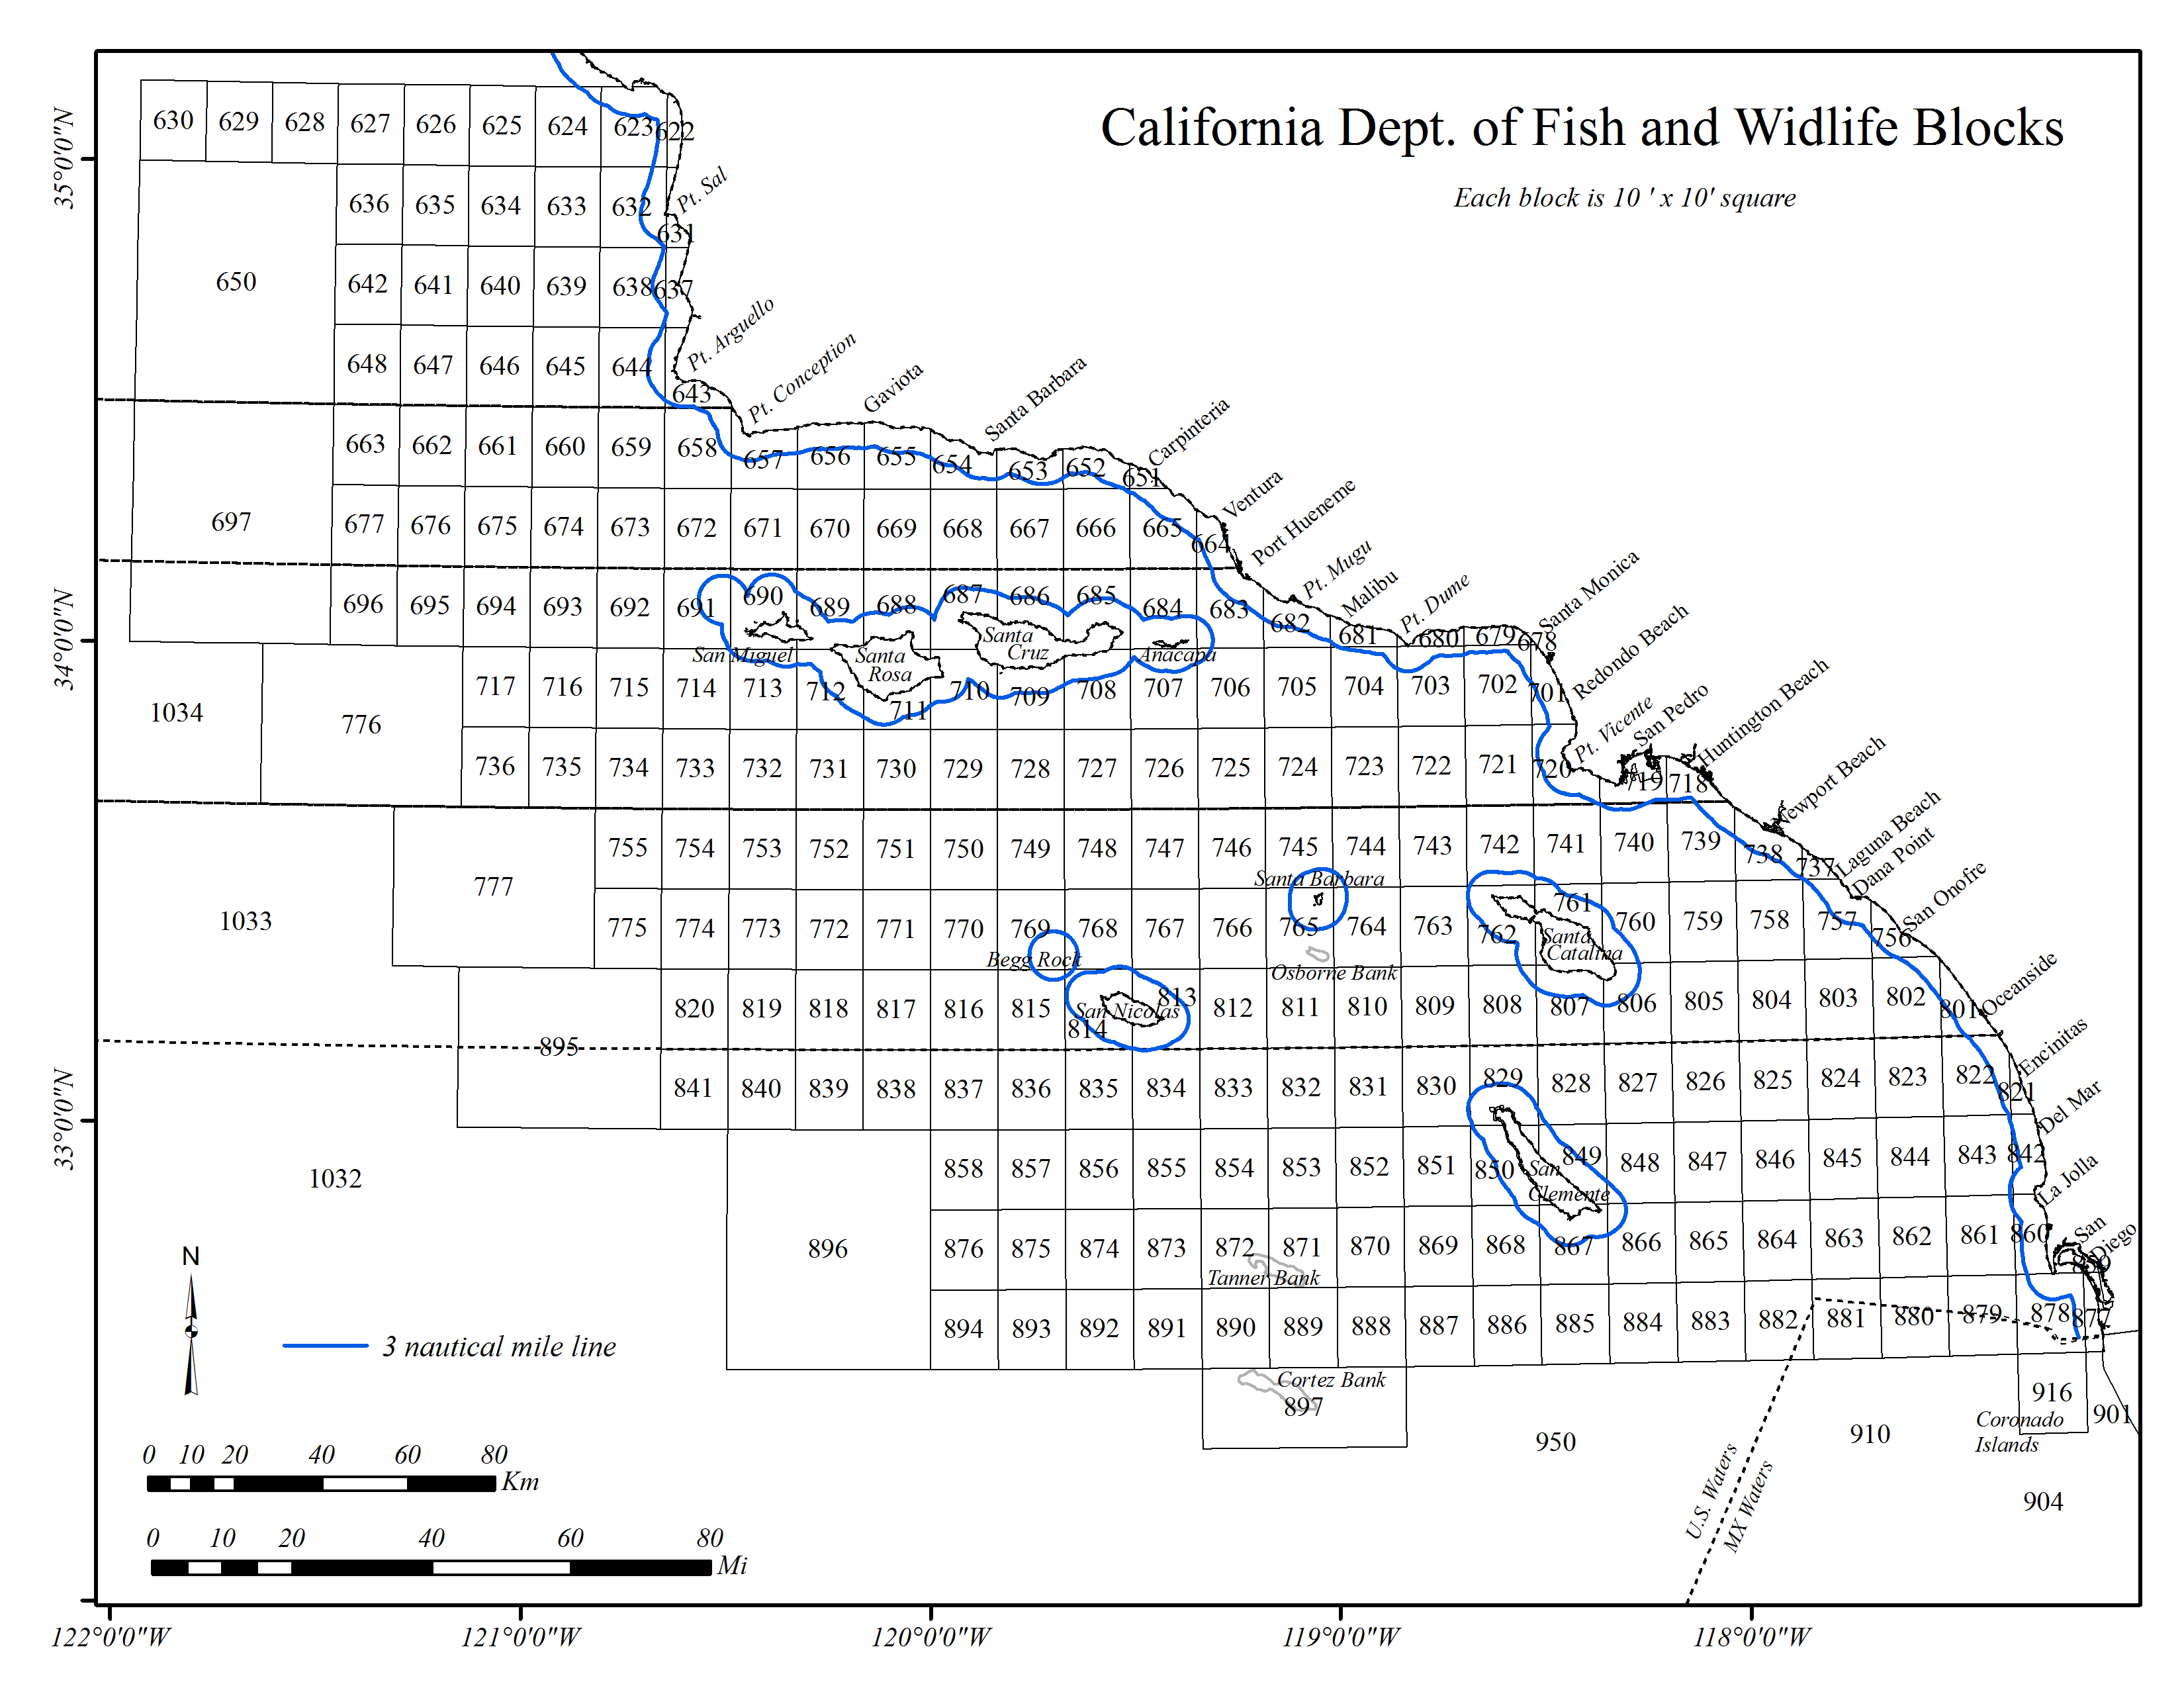
\includegraphics{Figures/boundary_map.png}
\caption{Map showing the state boundary lines for management of the
recreational fishing fleets. CRFS Districts 1-6 in California are
presented as well as the WDFW Recreational Management Areas in
Washington. Florence, OR is shown as a potential location of model
stratification. \label{fig:boundary_map}}
\end{figure}

\begin{figure}[htbp]
\centering
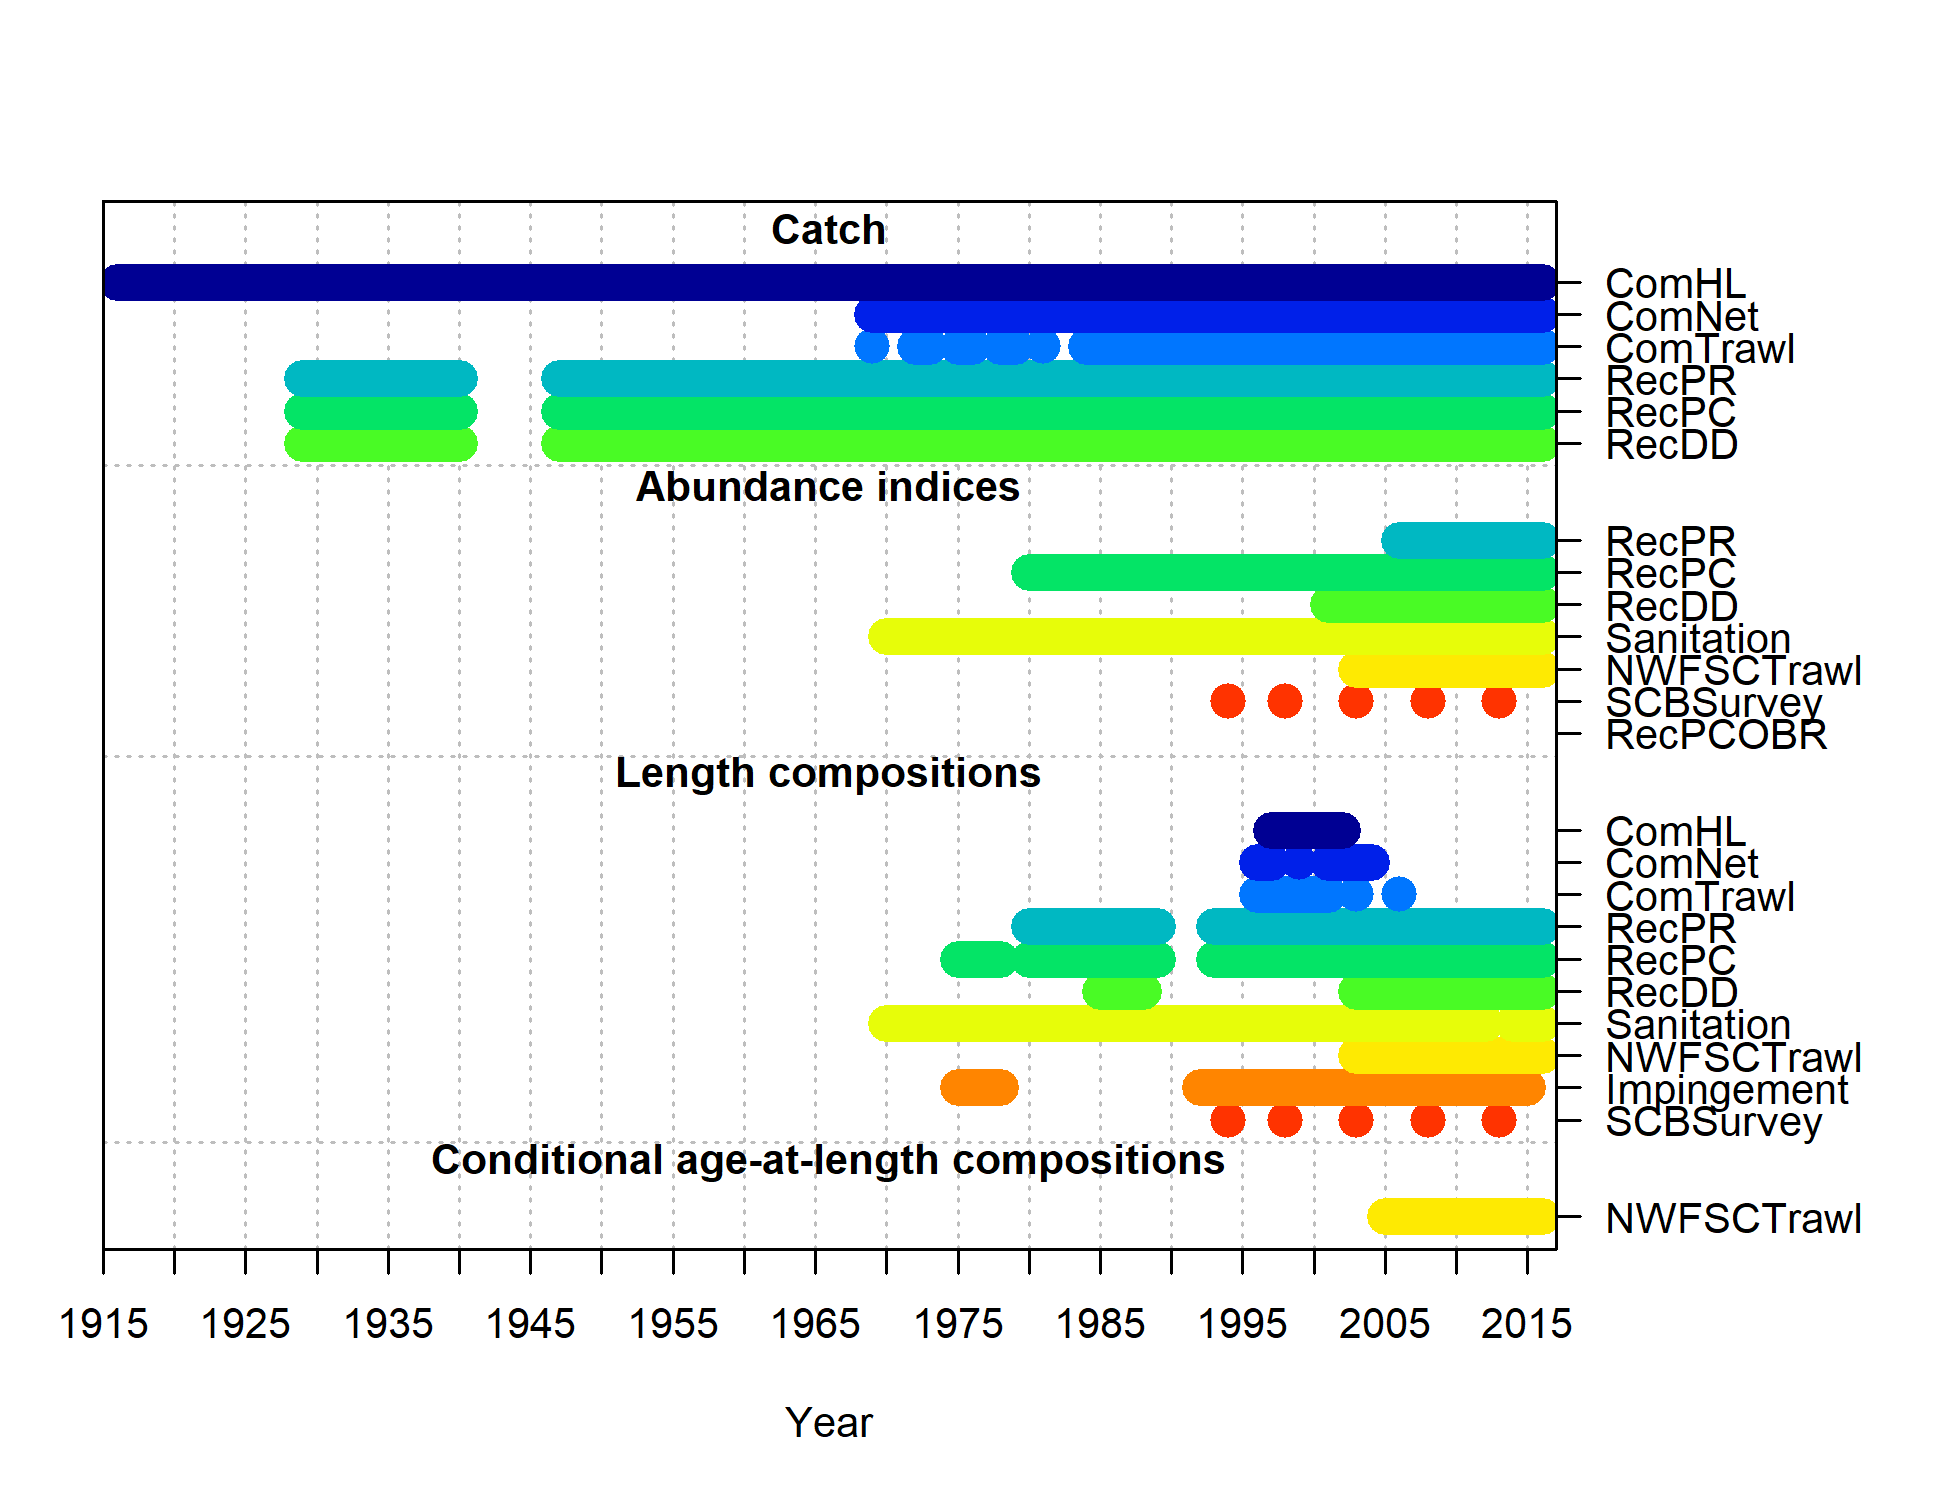
\includegraphics{r4ss/plots_mod1/data_plot.png}
\caption{Summary of data sources used in the base model.
\label{fig:data_plot}}
\end{figure}

\FloatBarrier

\FloatBarrier

\FloatBarrier

\FloatBarrier

\FloatBarrier

\FloatBarrier

\begin{figure}[htbp]
\centering
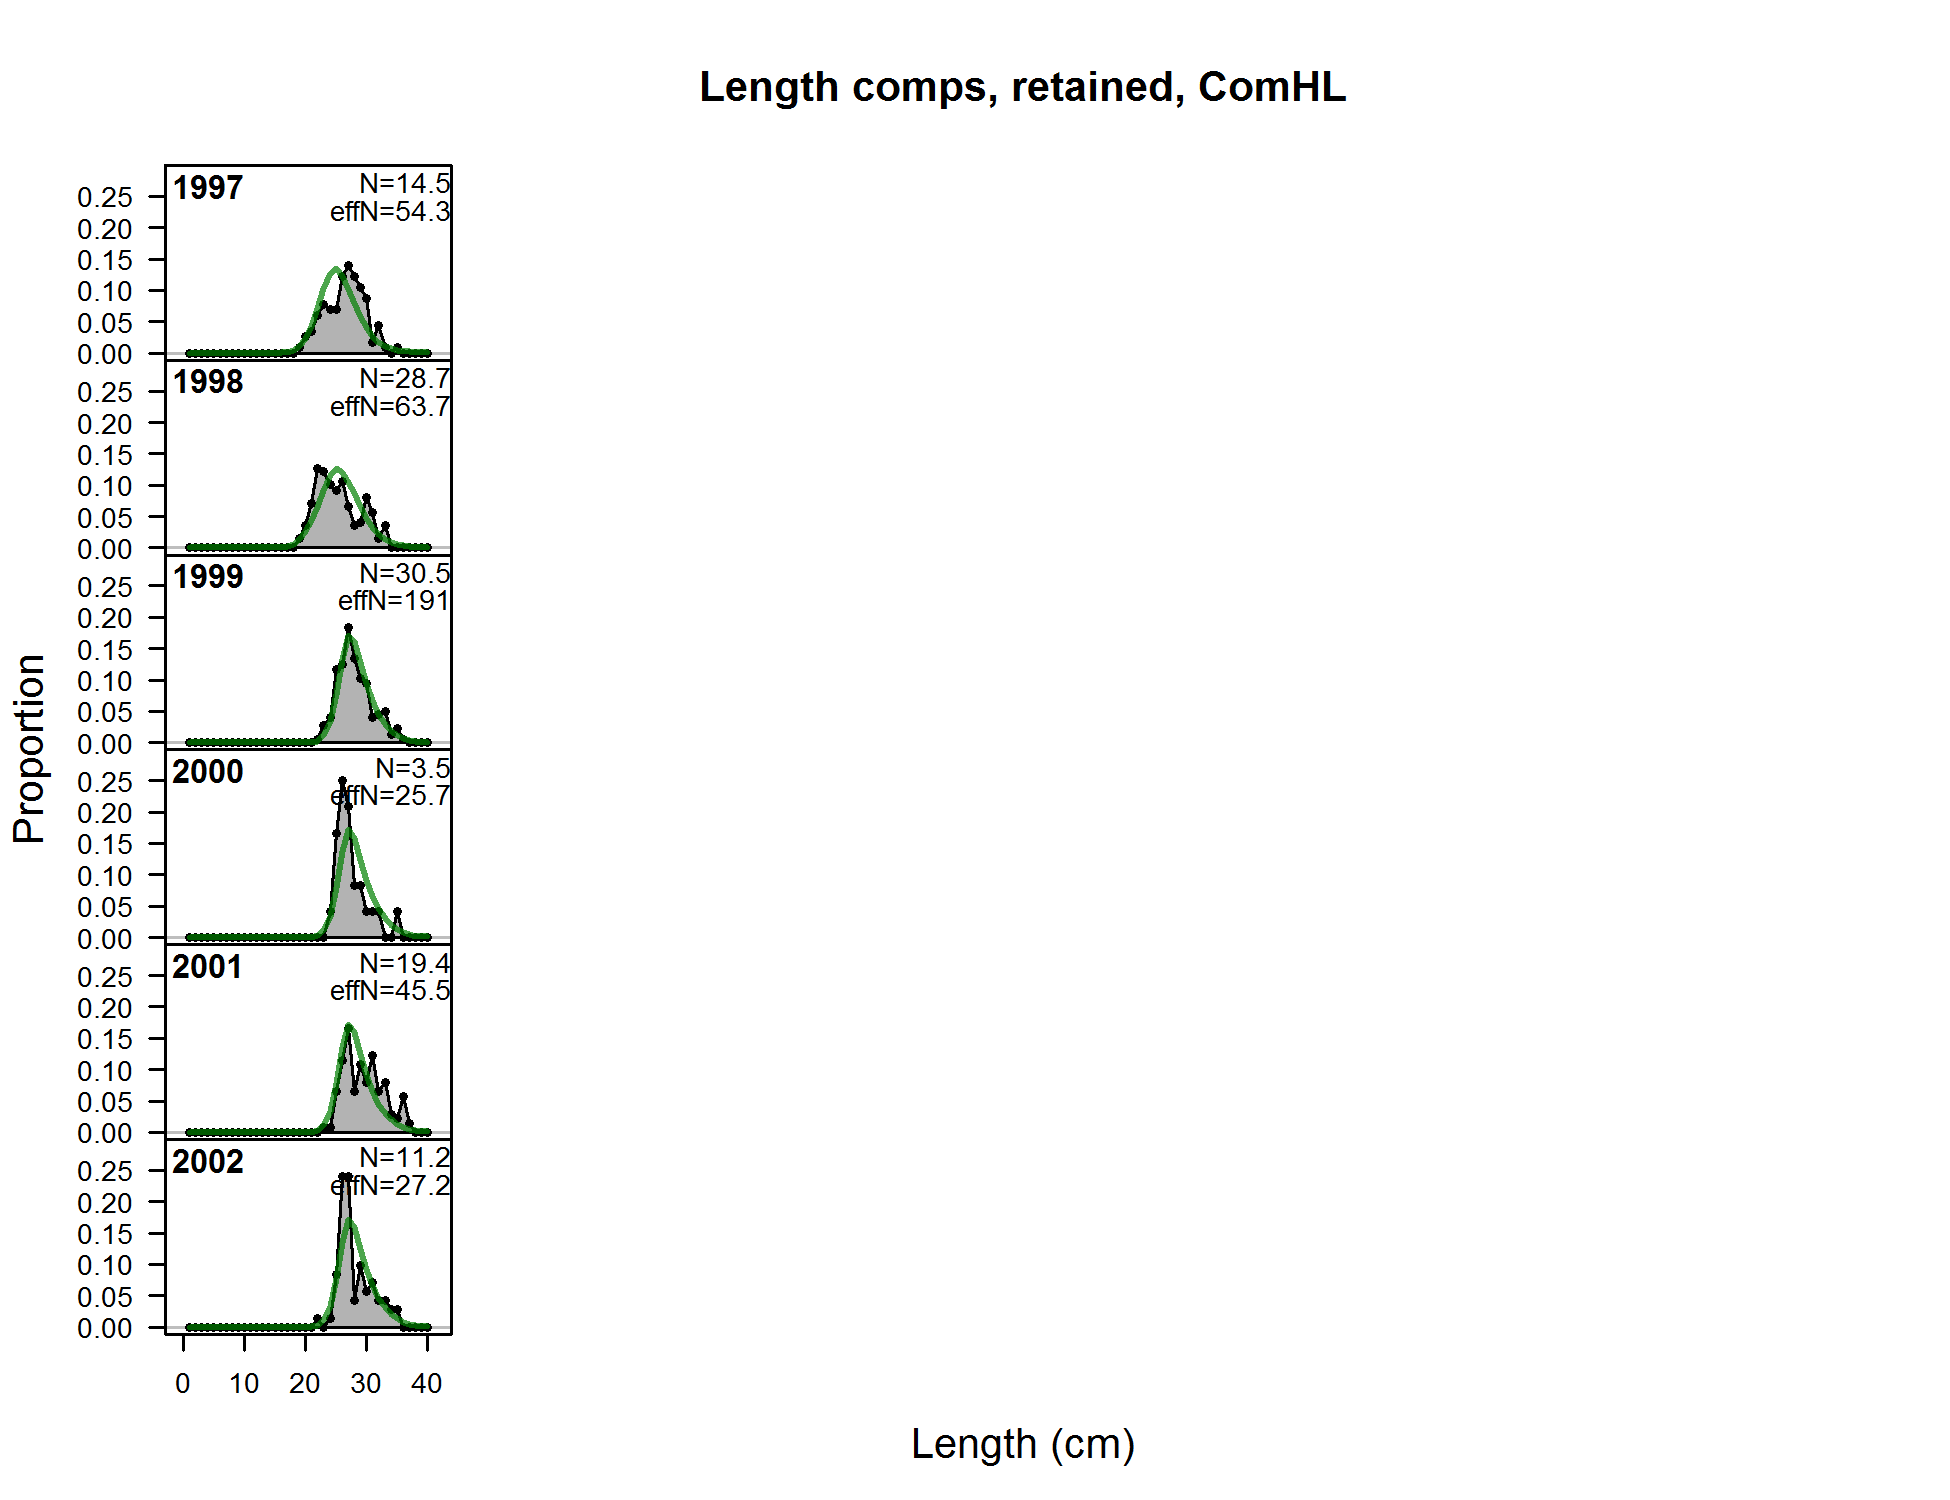
\includegraphics{./r4ss/plots_mod1/comp_lenfit_flt1mkt2.png}
\caption{Length comps, retained, ComHL
\label{fig:mod1_1_comp_lenfit_flt1mkt2}}
\end{figure}

\begin{figure}[htbp]
\centering
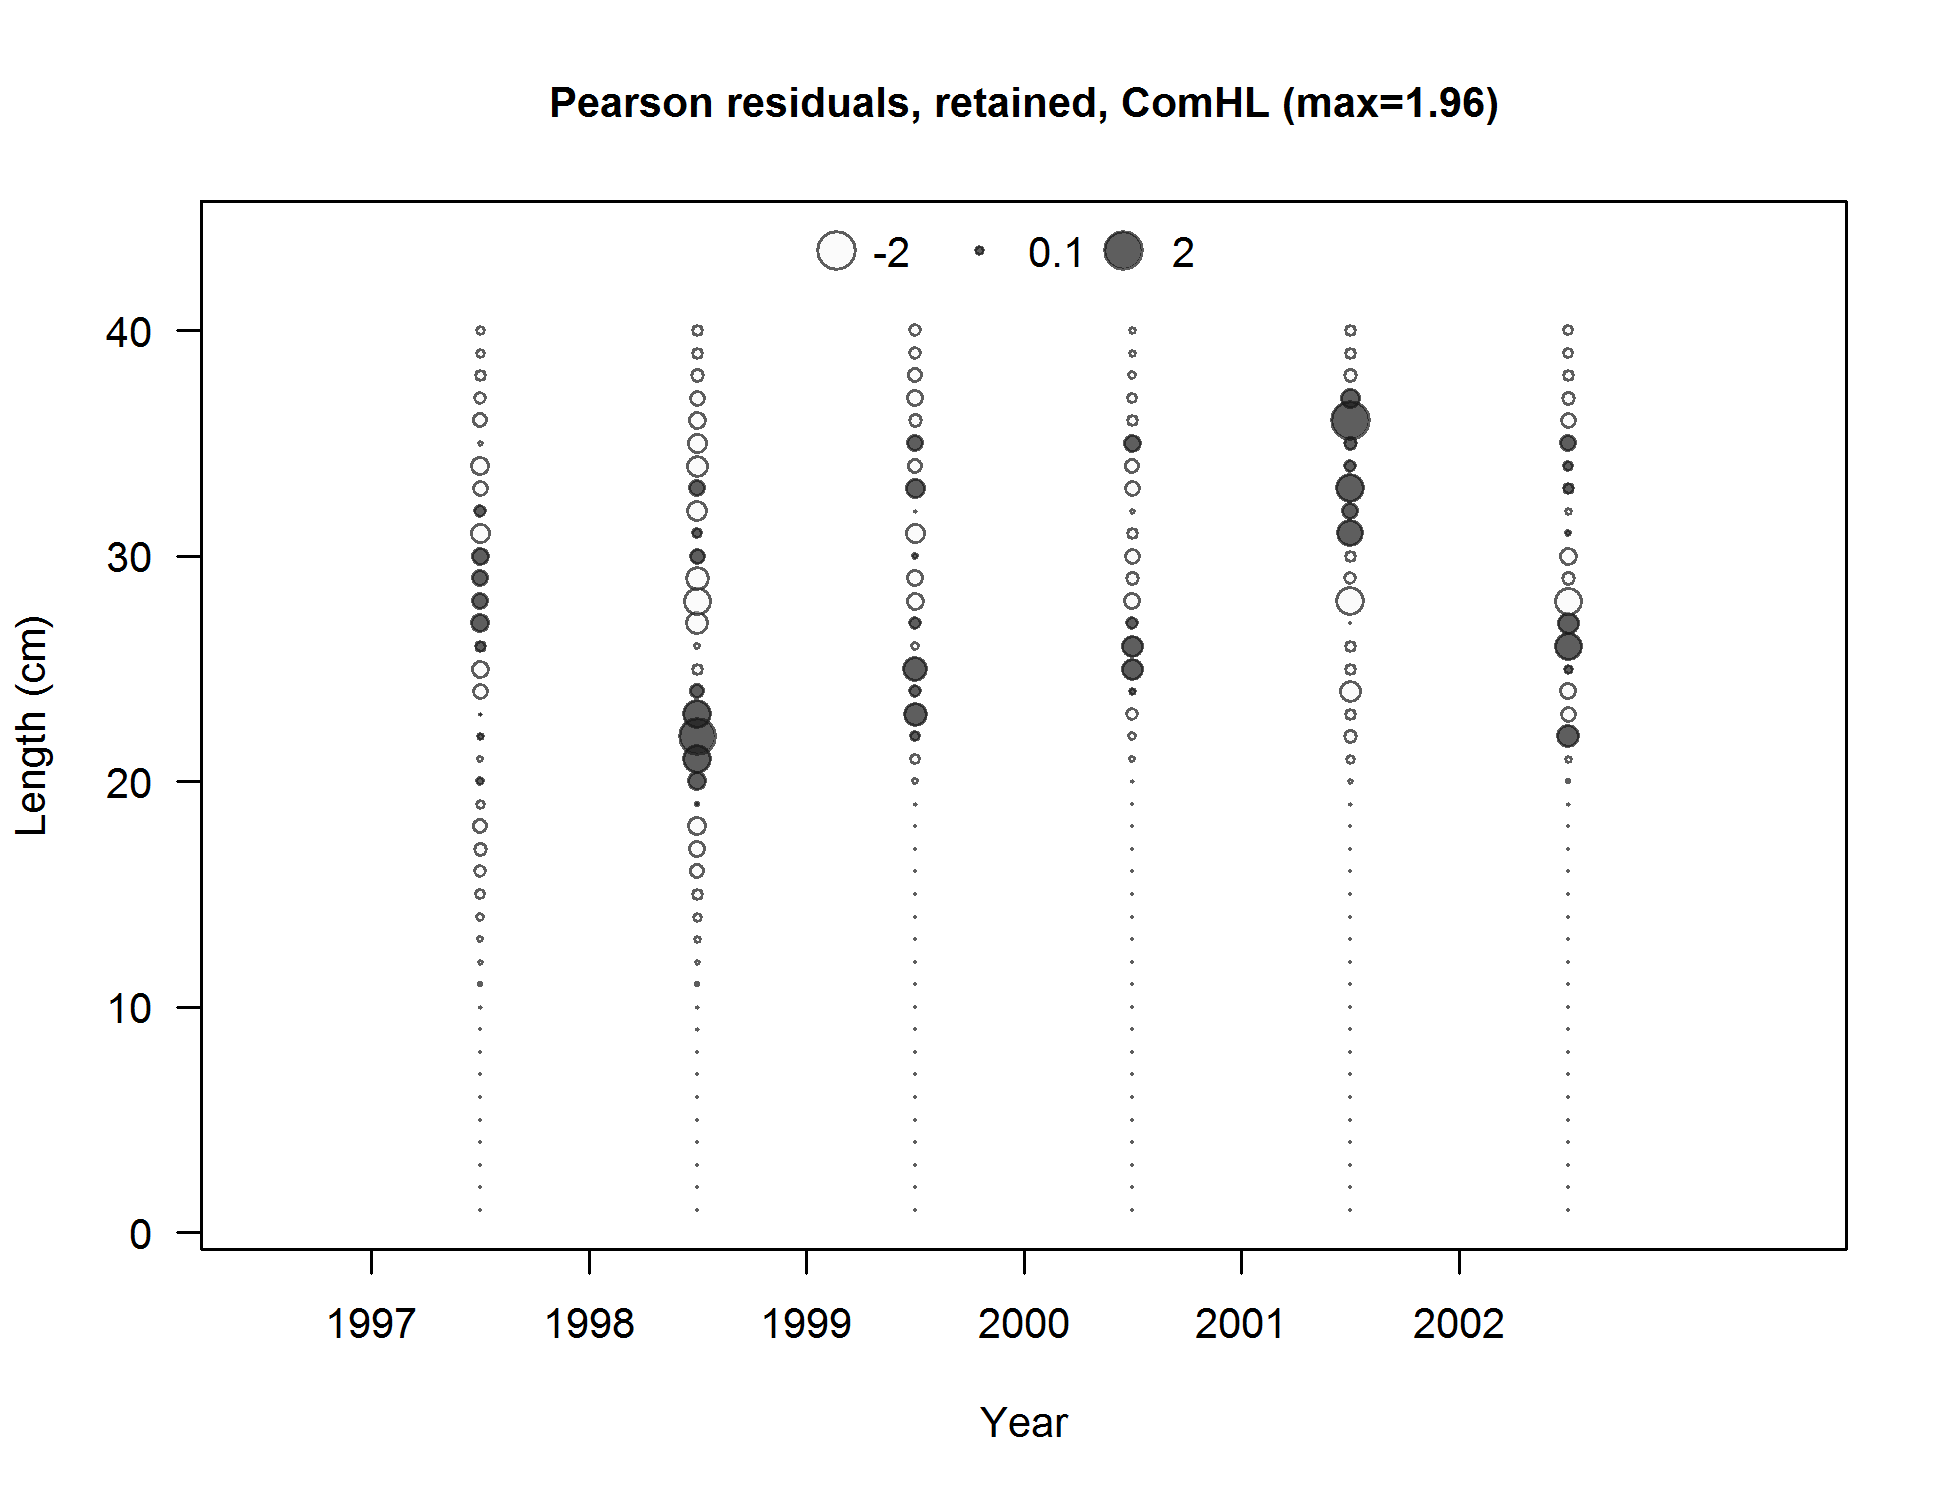
\includegraphics{./r4ss/plots_mod1/comp_lenfit_residsflt1mkt2.png}
\caption{Pearson residuals, retained, ComHL (max=7.96)\\
Closed bubbles are positive residuals (observed \textgreater{} expected)
and open bubbles are negative residuals (observed \textless{} expected).
\label{fig:mod1_2_comp_lenfit_residsflt1mkt2}}
\end{figure}

\begin{figure}[htbp]
\centering
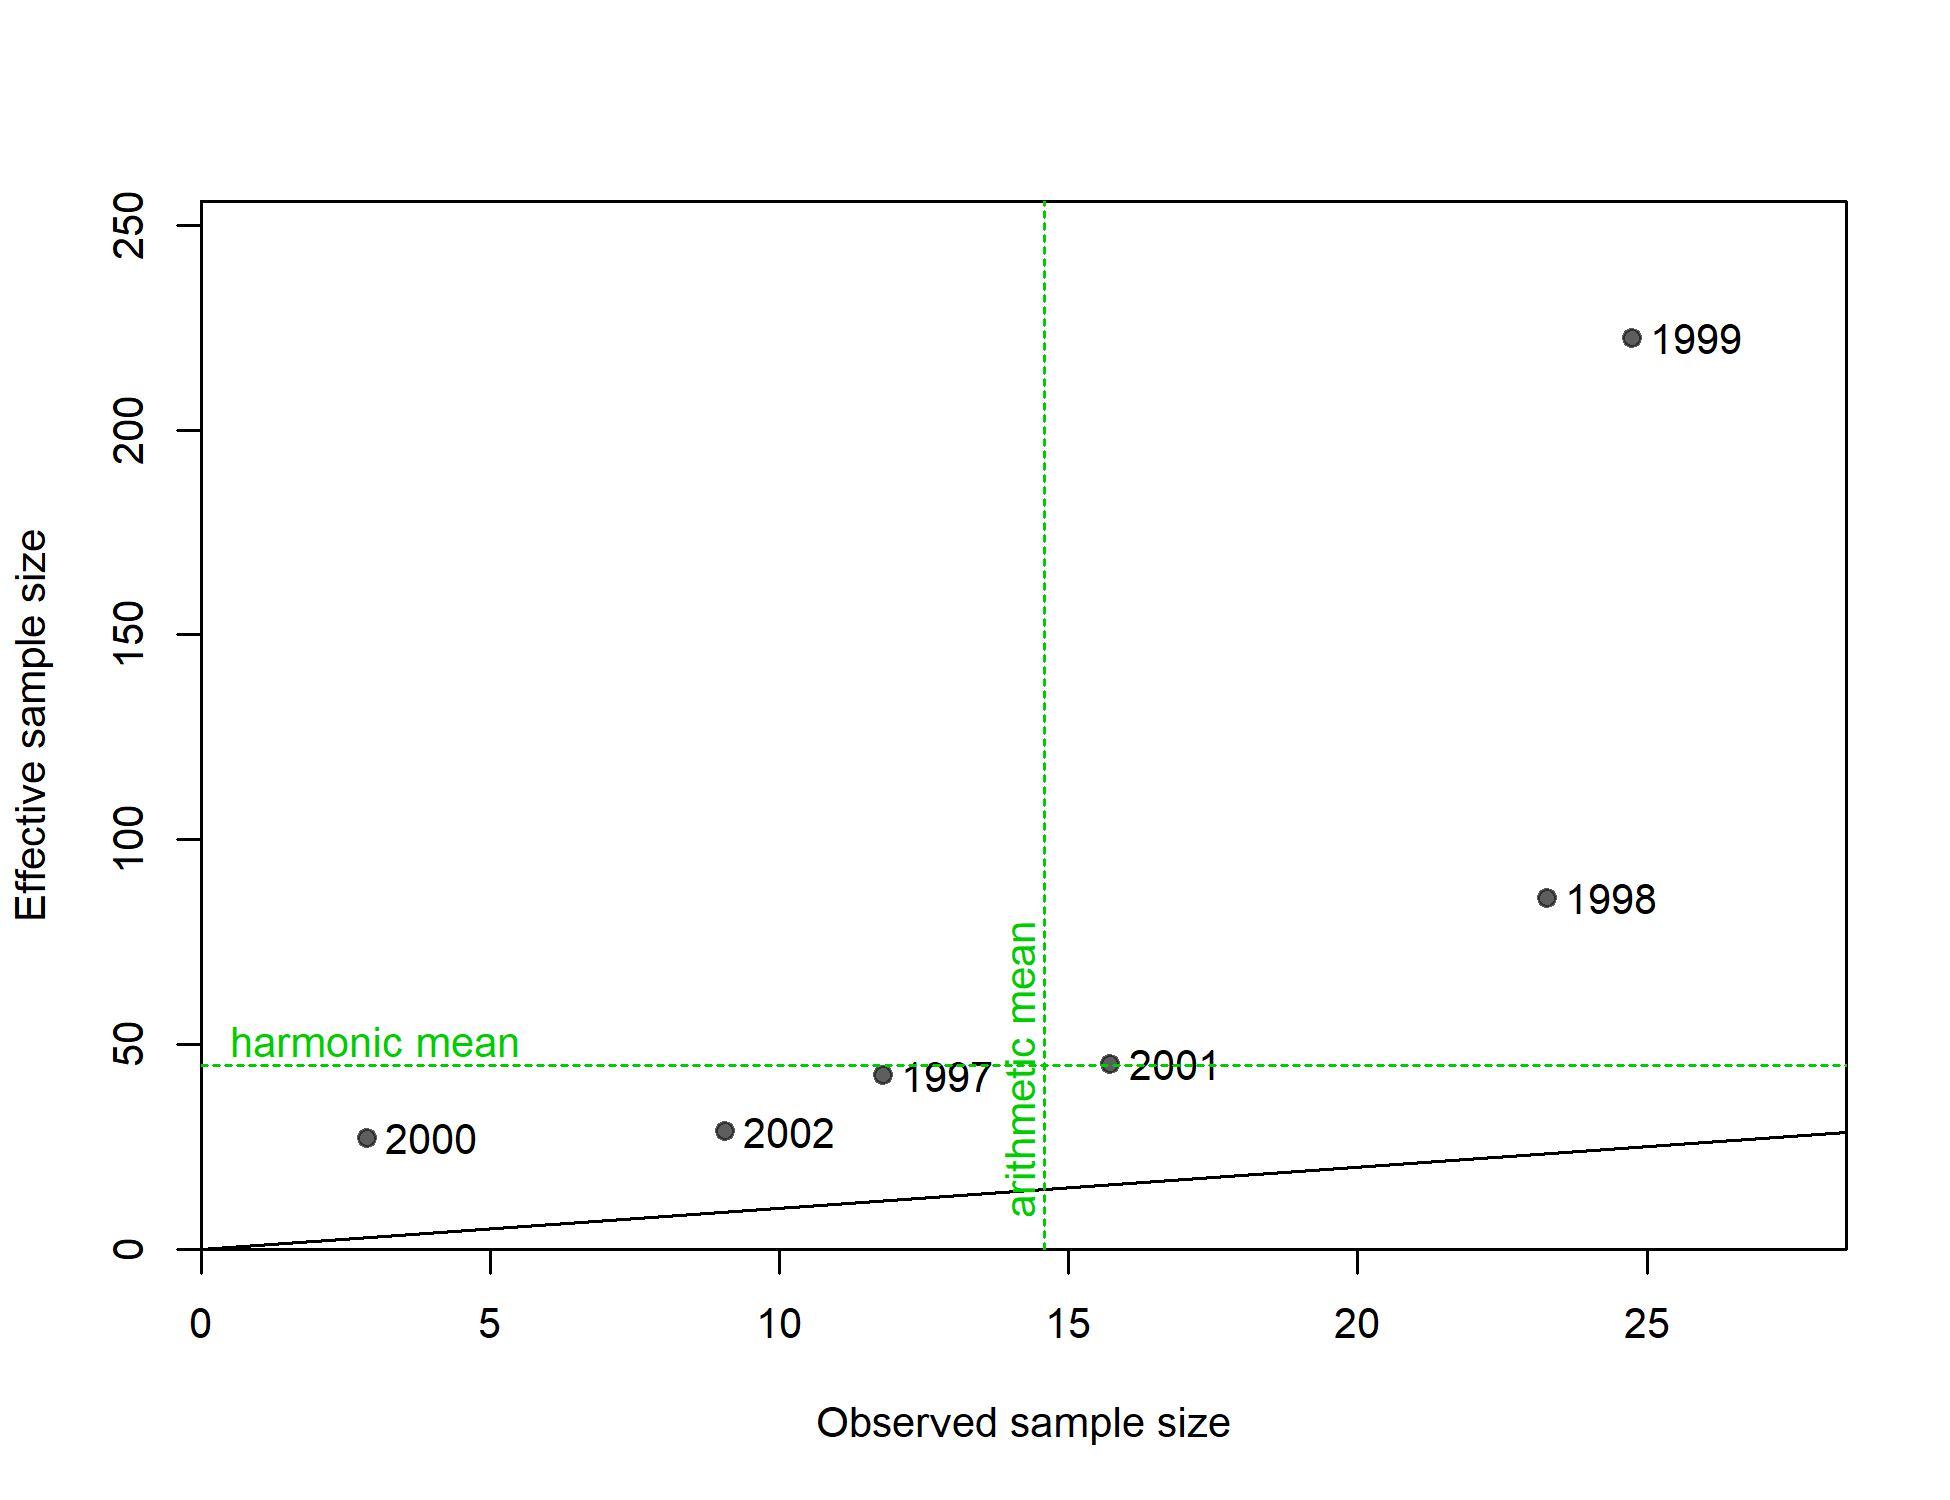
\includegraphics{./r4ss/plots_mod1/comp_lenfit_sampsize_flt1mkt2.png}
\caption{N\_EffN comparison, Length comps, retained, ComHL
\label{fig:mod1_3_comp_lenfit_sampsize_flt1mkt2}}
\end{figure}

\begin{figure}[htbp]
\centering
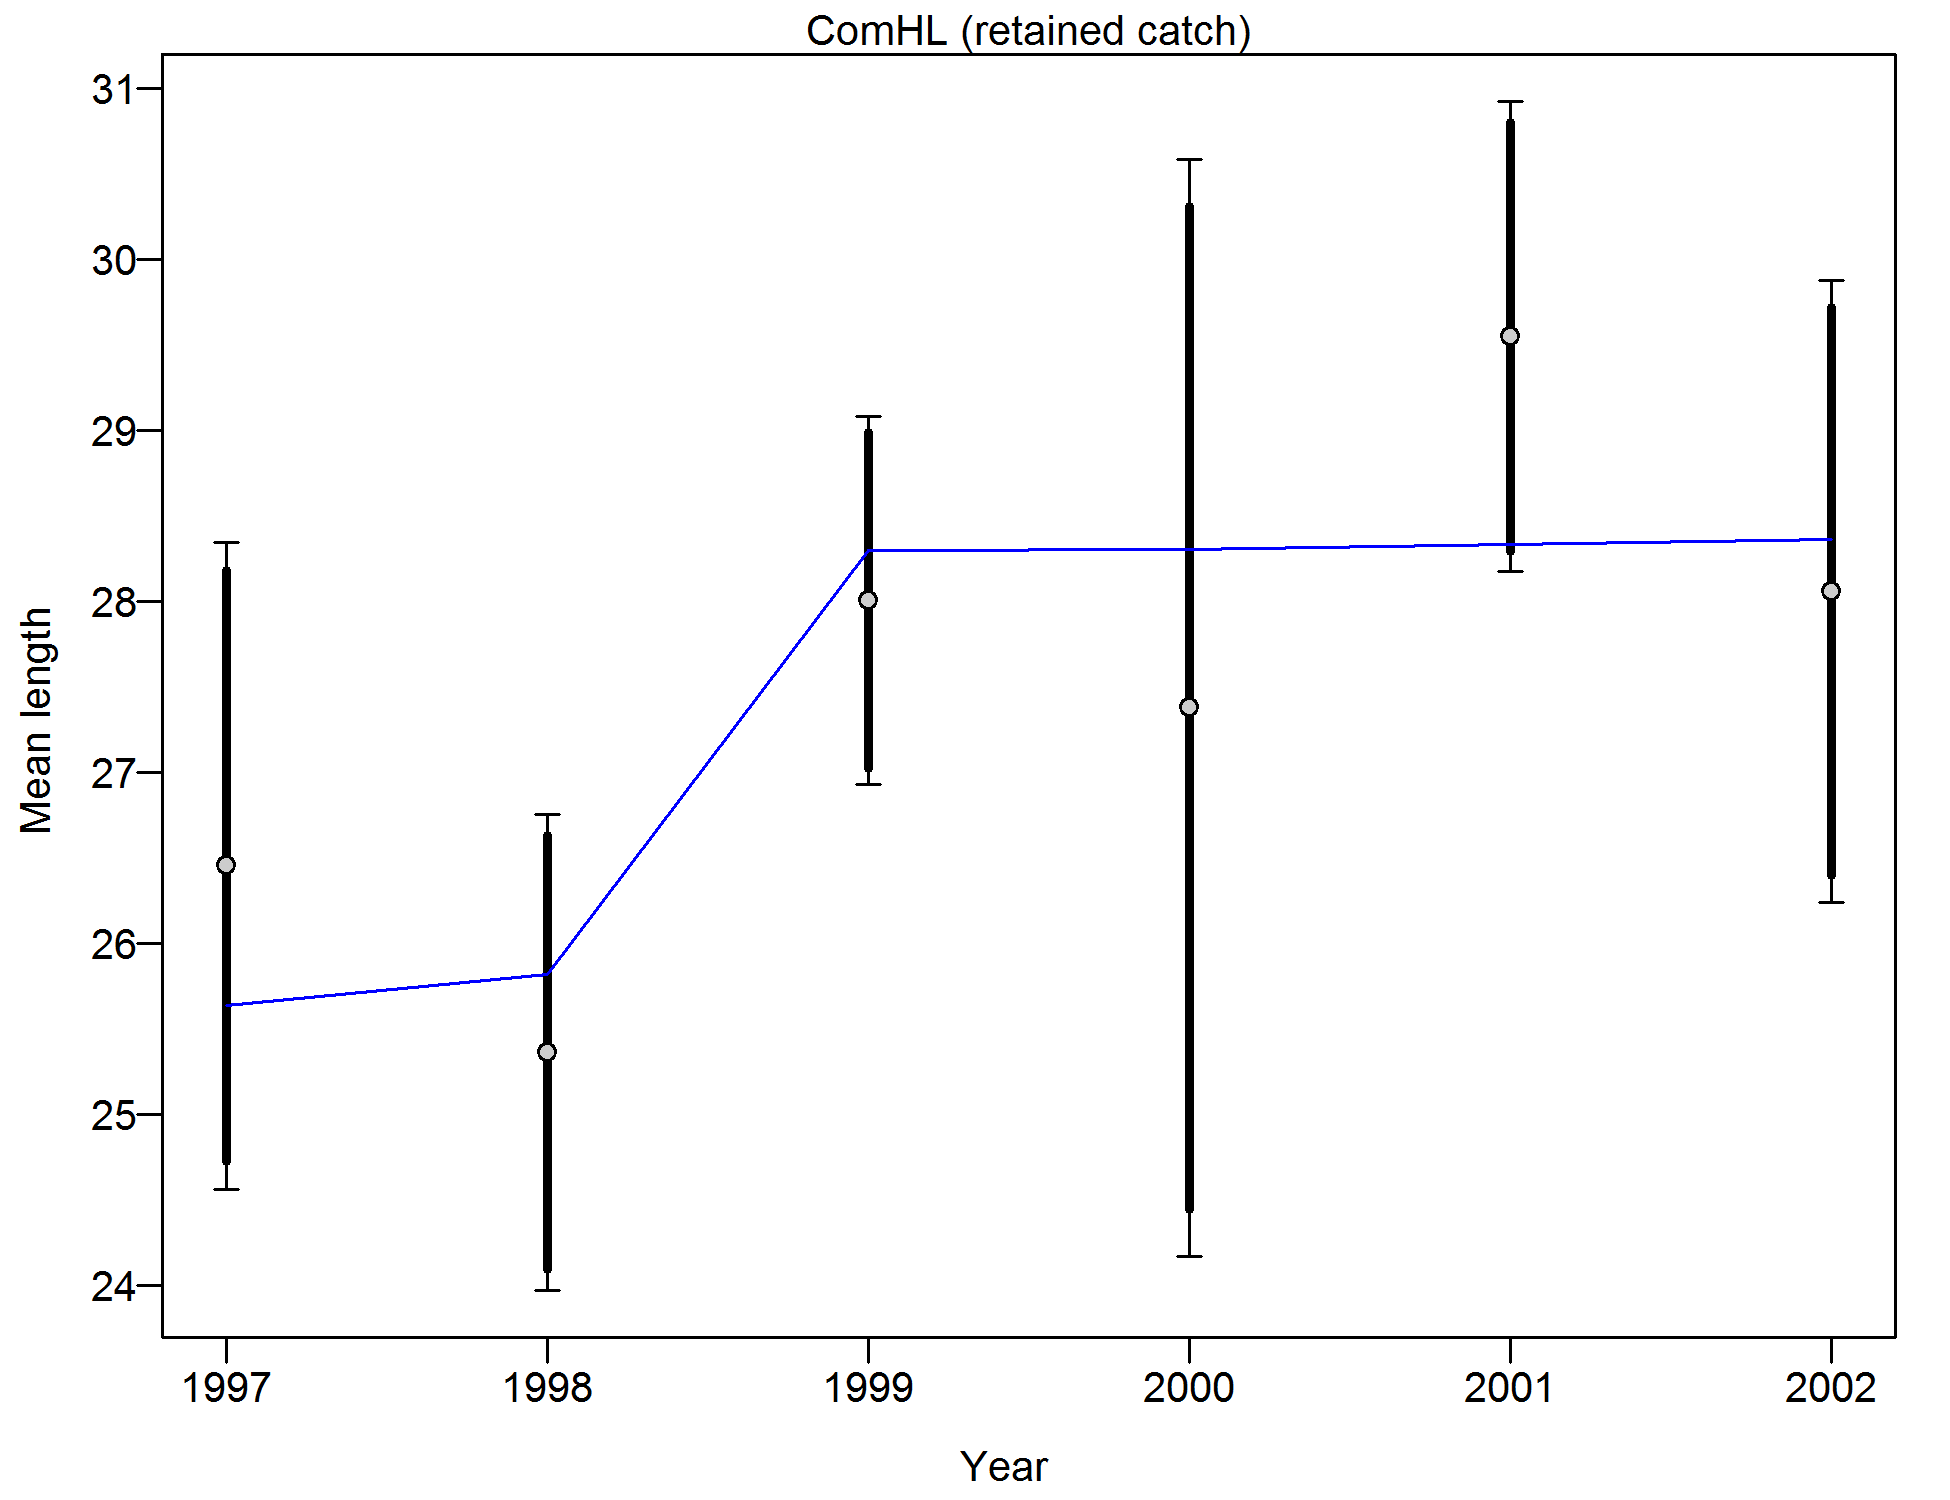
\includegraphics{./r4ss/plots_mod1/comp_lenfit_data_weighting_TA1.8_ComHL.png}
\caption{Francis data weighting method TA1.8: ComHL Suggested sample
size adjustment (with 95\% interval) for len data from ComHL: 0.197
(0.1179\_1.1745) For more info, see Francis, R.I.C.C. (2011). Data
weighting in statistical fisheries stock assessment models. Can. J.
Fish. Aquat. Sci. 68: 1124\_1138.
\label{fig:mod1_4_comp_lenfit_data_weighting_TA1.8_ComHL}}
\end{figure}

\begin{figure}[htbp]
\centering
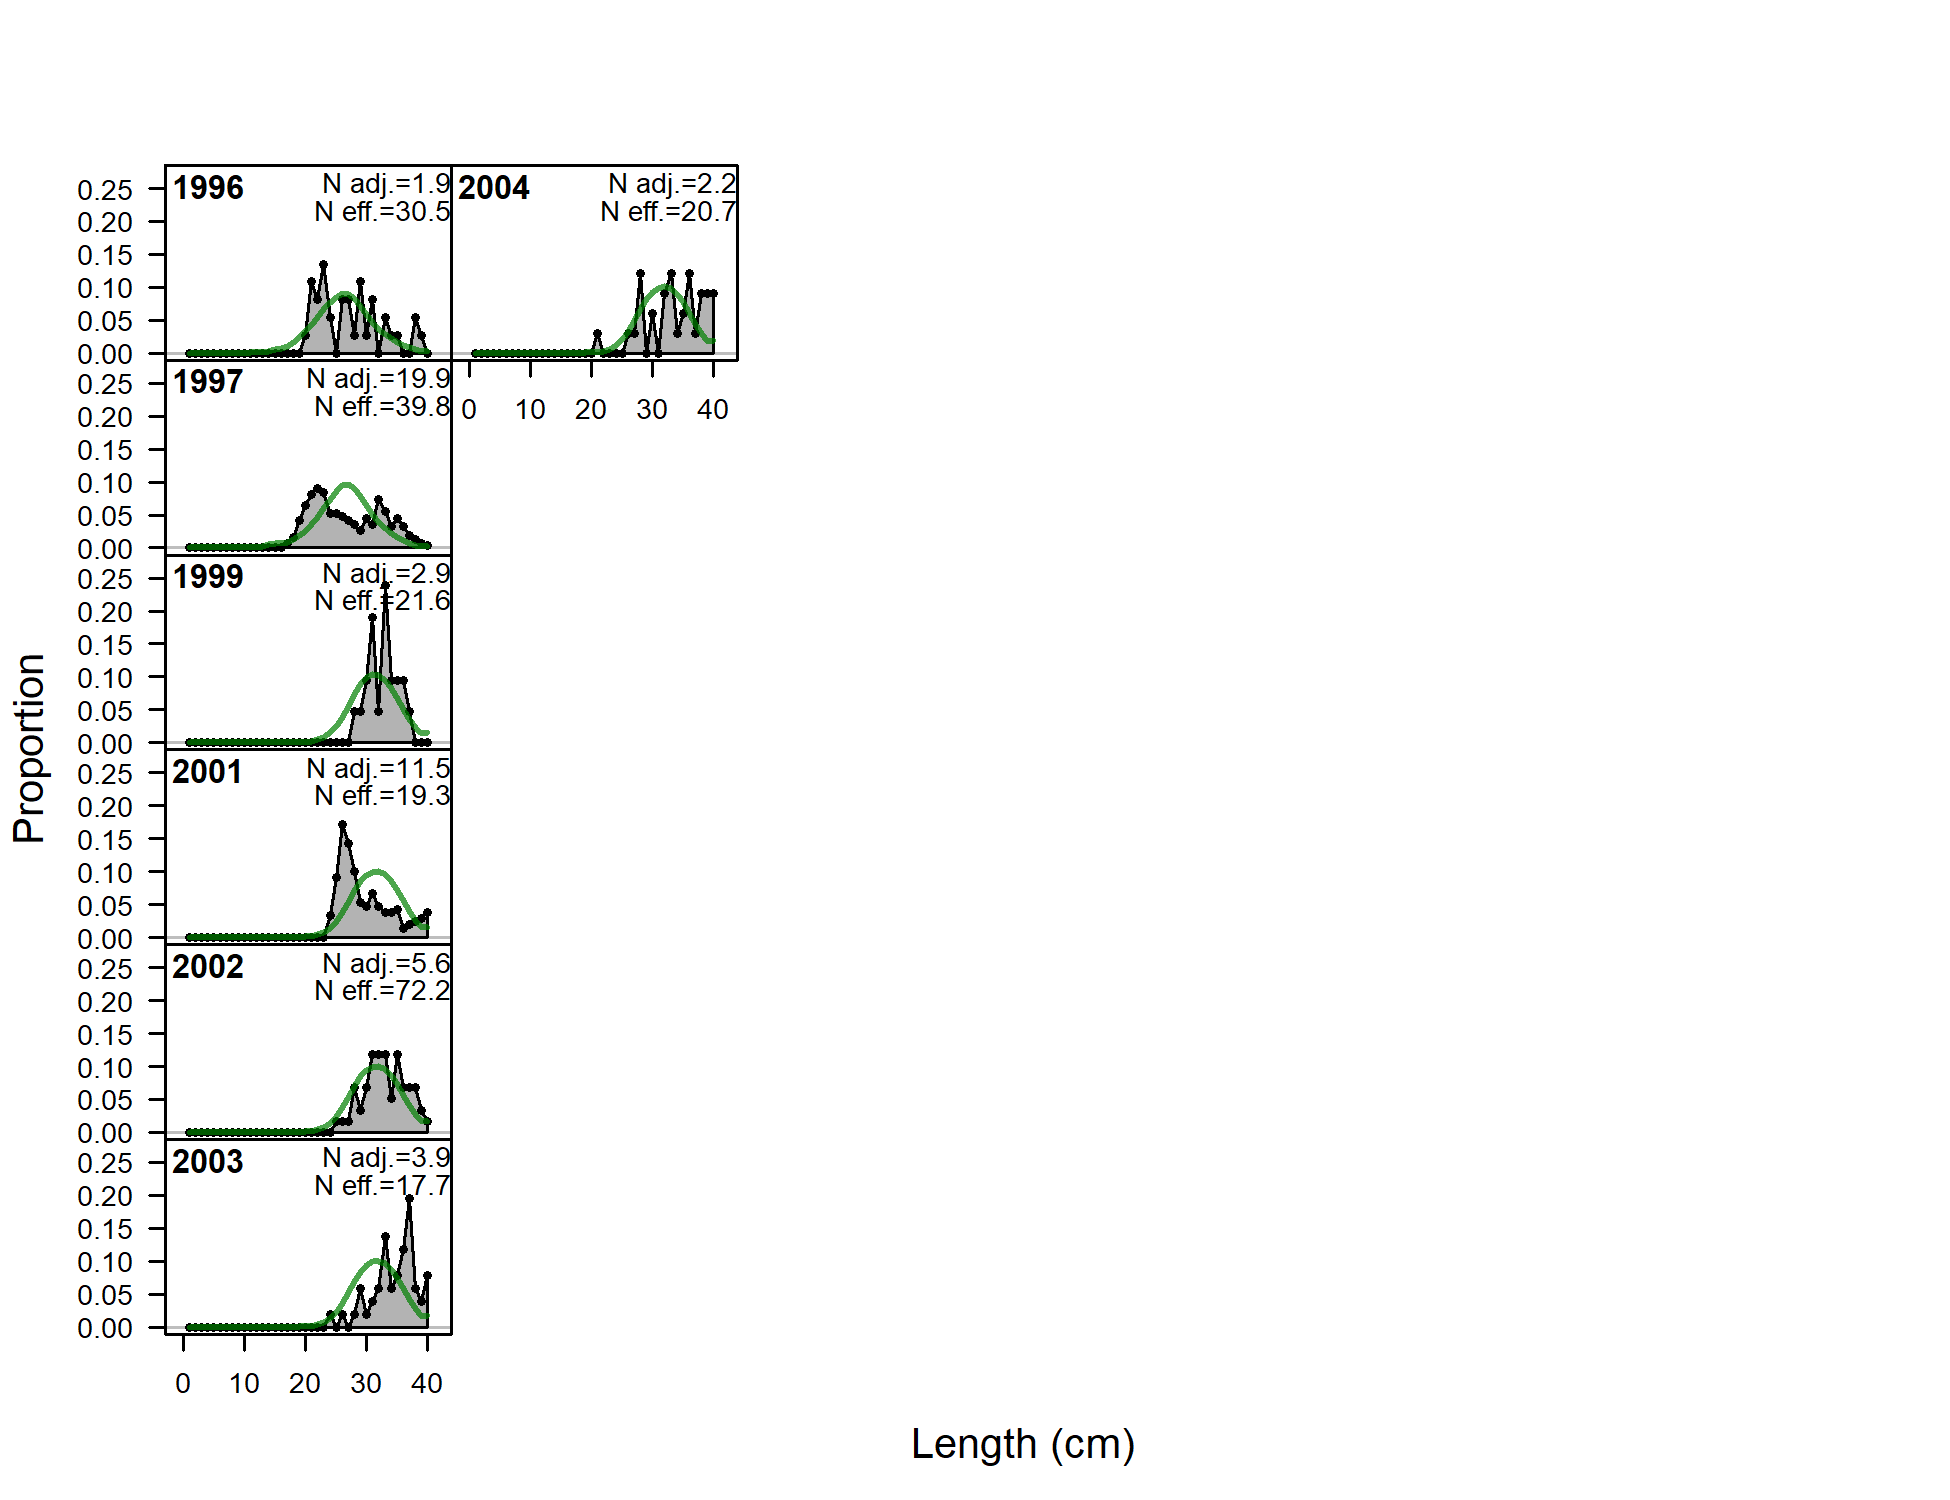
\includegraphics{./r4ss/plots_mod1/comp_lenfit_flt2mkt2.png}
\caption{Length comps, retained, ComNet
\label{fig:mod1_5_comp_lenfit_flt2mkt2}}
\end{figure}

\FloatBarrier

\FloatBarrier

\FloatBarrier

\FloatBarrier

\FloatBarrier

\FloatBarrier

\FloatBarrier

\newpage

\color{black}

\section*{References}\label{references}
\addcontentsline{toc}{section}{References}

\renewcommand{\thepage}{}

\hypertarget{refs}{}
\hypertarget{ref-Alverson1964}{}
Alverson, D.L., Pruter, a T., and Ronholt, L.L. 1964. A Study of
Demersal Fishes and Fisheries of the Northeastern Pacific Ocean.
Institute of Fisheries, University of British Columbia.

\hypertarget{ref-vonB1938}{}
Bertalanffy, L. von. 1938. A quantitative theory of organic growth.
Human Biology \textbf{10}: 181--213.

\hypertarget{ref-Eschmeyer1983}{}
Eschmeyer, W.N., Herald, E., and Hammann, H. 1983. A field guide to
Pacific coast fishes of North America. Houghton Mifflin Company, Boston,
MA.

\hypertarget{ref-Francis2011}{}
Francis, R. 2011. Data weighting in statistical fisheries stock
assessment models. Canadian Journal of Fisheries and Aquatic Sciencies
\textbf{68}: 1124--1138.

\hypertarget{ref-Frey1971}{}
Frey, H. (n.d.). California's living marine resources and their
utilization. California Department of Fish; Game, Sacramento, CA.

\hypertarget{ref-Hamel2015}{}
Hamel, O. 2015. A method for calculating a meta-analytical prior for the
natural mortality rate using multiple life history correlates. ICES
Journal of Marine Science \textbf{72}: 62--69.

\hypertarget{ref-Harry1961}{}
Harry, G., and Morgan, A. 1961. History of the trawl fishery, 1884-1961.
Oregon Fish Commission Research Briefs \textbf{19}: 5--26.

\hypertarget{ref-Love2002}{}
Love, M., Yoklavich, M., and Thorsteinson, L. 2002. The rockfishes of
the northeast Pacific. University of California Press, Berkeley, CA,
USA.

\hypertarget{ref-Love1987}{}
Love, M.S., Axell, B., Morris, P., Collins, R., and Brooks\(\sim\)-, A.
1987. Life history and fishery of the California scorpionfish,
\emph{Scorpaena guttata}, within the Southern California Bight. Fishery
Bulletin \textbf{85}: 99--116.

\hypertarget{ref-Maunder2005}{}
Maunder, M.N., Barnes, T., Aseltine-Neilson, D., and MacCall, A.D. 2005.
The status of California scorpionfish (\emph{Sorpaena guttata}) off
southern California in 2004. Pacific Fishery Management Council,
Portland, OR.

\hypertarget{ref-McAllister1997}{}
McAllister, M.K., and Ianelli, J.N. 1997. Bayesian stock assessment
using catch-age data and the sampling - importance resampling algorithm.
Canadian Journal of Fisheries and Aquatic Sciences \textbf{54}(2):
284--300.

\hypertarget{ref-Methot2015}{}
Methot, R.D. 2015. User manual for Stock Synthesis model version 3.24s.
NOAA Fisheries, US Department of Commerce.

\hypertarget{ref-Moser1996}{}
Moser, H. (n.d.). Scorpaenidae \emph{Scorpaena guttata}. \emph{In}
CalCOFI atlas 33: The early stages of the fishes in the califonria
current region. pp. 788--789.

\hypertarget{ref-Moser2002}{}
Moser, H. G., R. L. Charter, P. E. Smith, D. A. Ambrose, W. Watson,
S.R., Charter, and Sandknop, E.M. 2002. Atlas 35: Distributional atlas
of fish larvae and eggs from Manta (surface) samples collected on
CalCOFI surveys from 1977 to 2000. California Cooperative Oceanic
Fisheries Investigations.

\hypertarget{ref-Orton1955}{}
Orton, G. 1955. Early developmental stages of the California
scorpionfish, \emph{Scorpaena guttata}. Copeia: 210--214.

\hypertarget{ref-PFMC1993}{}
Pacific Fishery Management Council (Institution/Organization). 1993. The
Pacific Coast Groundfish Fishery Management Plan: Fishery Management
Plan for the California, Oregon, and Washington Groundfish Fishery as
Amended Through Amendment 7. Pacific Fishery Management Council,
Portland, OR.

\hypertarget{ref-PFMC2002}{}
Pacific Fishery Management Council (Institution/Organization). 2002.
Status of the Pacific Coast Groundfish Fishery Through 2001 and
Acceptable Biological Catches for 2002: Stock Assessment and Fishery
Evaluation. Pacific Fishery Management Council, Portland, OR.

\hypertarget{ref-PFMC2004}{}
Pacific Fishery Management Council (Institution/Organization). 2004.
Pacific Coast Groundfish Fishery Management Plan: Fishery Management
Plan for the California, Oregon, and Washington Groundfish Fishery as
Amended Through Amendment 17. Pacific Fishery Management Council,
Portland, OR.

\hypertarget{ref-Quast1968}{}
Quast, J. 1968. Observations on the food of the kelp-bed fishes.
California Department of Fish and Game Fish Bulletin (139): 109--142.

\hypertarget{ref-Taylor1963}{}
Taylor, P. 1963. The venom and ecology of the California scorpionfish,
Scorpaena guttata Girard. PhD Thesis, University of California San
Diego.

\hypertarget{ref-Then2015}{}
Then, A., Hoenig, J., Hall, N., and Hewitt, D. 2015. Evaluating the
predictive performance of empirical estimators of natural mortality rate
using information on over 200 fish species. ICES Journal of Marine
Science \textbf{72}: 82--92.

\hypertarget{ref-Turner1969}{}
TuRNER, C.H., EBERT, E.E., and GIVEN, R.R. (n.d.). Man-mae reef ecology.
California Department of Fish and Game Fish Bulletin \textbf{146}: 221.

\hypertarget{ref-Washington1984}{}
Washington, B., Moser, H.G., Laroche, W.A., and W. J. Richards, J.
(n.d.). Scorpaeniformes: development. \emph{In} Ontogeny and systematics
of fishes. american society of ichthyologists and herpetologists special
publication 1. \emph{Edited by} H. G., A.W. Moser, W. J. Richards, D. M.
Cohen, M. P. Fahay, J. Kendall, and S.L. Richardson. pp. 405--428.

\end{document}
